  \documentclass[journal]{IEEEtran}
  \usepackage{amsmath,amssymb}
  \usepackage{booktabs}
  \usepackage{multirow}
  \usepackage{graphicx}
\usepackage{float}
  \usepackage{url}
  \usepackage{array}
  \usepackage{cite}
  \usepackage{enumitem}
  \usepackage{balance}
  \usepackage{hyperref}
  \usepackage{tikz}
  \usetikzlibrary{arrows.meta,positioning}
  \hypersetup{hidelinks}
  \graphicspath{{figures/}{../reports/}{experiment_cpaisd/reports/}{experiment_cpaisd/paper/figures/}}
  
  \title{Integrity Verification and Anomaly Detection for DICOM Brain CT: Controlled Tampering and Signed-Manifest Evaluation}
  
  \author{Aditya Upendra Gupta, Aaditya Awasthi, Nidal, and Sudhawalli\\
  \thanks{This manuscript reports an exploratory, single-dataset experiment using CPAISD. It is not a clinical validation study.}}
  
  \begin{document}
  \maketitle
  
  \begin{abstract}
Digital Imaging and Communications in Medicine (DICOM) objects combine image pixels with metadata used to identify, organize, and interpret imaging studies. This paper reports controlled metadata and pixel-integrity experiments and a signed-manifest transfer-security prototype on CPAISD non-contrast brain CT. The official train/validation/test folds contain 92/10/10 studies (8,376/980/809 instances). Across six scripted metadata conditions, reference SHA-256 achieved macro F1 1.000 using each exact clean test file as its reference; the autoencoder and Isolation Forest achieved 0.506 and 0.116. An Adam-bilevel metadata autoencoder learned numerical/categorical/presence loss weights of 0.206/0.430/0.364, but its file macro F1 (0.562) was only slightly above matched MSE (0.557), and clean-test FPR remained 21.1\%. A separate 11-setting, three-seed loss-weight sweep found that no setting met a 2\% held-out validation FPR target in all seeds. Study/series rules detected single-slice conflicts but missed a coordinated study-wide edit. For pixel localization, bilevel WBCE--Dice weighting improved IoU to 0.628 from 0.456 with fixed equal weights, while image F1 decreased from 0.913 to 0.884 and clean-image FPR increased from 5.19\% to 6.43\%. In a 13-scenario signed-manifest evaluation on all 809 test files, each scenario produced its expected verification outcome; mean signing and end-to-end verification times were 15.44 and 12.82 ms/file. Attention U-Net results varied by edit family, and bounded white-box attacks reduced localization performance. All attacks were synthetic; network throughput, live DICOM transport, clinical utility, and external generalization remain unestablished.
  \end{abstract}
  
  \begin{IEEEkeywords}
  DICOM, metadata integrity, digital signatures, HMAC-SHA256, secure medical image exchange, semantic consistency, anomaly detection, computed tomography.
  \end{IEEEkeywords}
  
  \section{Introduction}
  \IEEEPARstart{M}{edical} imaging workflows depend on DICOM objects to transport and store pixel arrays together with attributes describing the patient, study, series, acquisition, and equipment. Metadata is operationally important: identifiers associate instances with a patient and study, while technical attributes can affect image interpretation, measurement, routing, and downstream processing. A file may therefore undergo a metadata change without a visible change to its pixel data. Security mechanisms that inspect only image appearance will not necessarily detect such a change.
  
  Cryptographic integrity mechanisms, digital signatures, and reversible watermarking have been studied for DICOM authenticity and tamper detection. DICOM PS3.15 specifies security and system-management profiles, including digital-signature and audit-trail profiles \cite{dicomps315}. These methods typically rely on a reference, key, signature, or embedded watermark. Statistical anomaly detectors offer a different capability: they can flag values that depart from patterns learned from clean data, even when an exact trusted original is not available. Their limitation is that statistical unusualness is not equivalent to maliciousness, and a plausible but incorrect change may not be anomalous.
  
  This work evaluates these complementary mechanisms on CPAISD, a public cohort of hyperacute ischemic-stroke non-contrast CT studies. The objectives are to: (i) compare reference hashing, structural rules, study/series consistency checks, and unsupervised detectors on controlled metadata edits; (ii) assess no-reference pixel anomaly baselines and supervised localization on synthetic pixel masks; (iii) compare metadata reconstruction objectives and fixed versus bilevel loss-group weights; (iv) compare fixed, directly learned, and bilevel WBCE--Dice weighting for pixel localization; (v) characterize bounded white-box evasion and paired metadata-plus-pixel integrity checks; and (vi) implement and evaluate sender--receiver verification using signed DICOM sidecar manifests. The contribution is a reproducible, dataset- and protocol-specific implementation and comparison, not a new cryptographic primitive, anomaly algorithm, or image-localization detector. Prior DICOM integrity and watermark-based localization work precludes a broad claim of first-ever tamper detection \cite{kobayashi2009,tan2011,dou2012,alhaj2015,oh2026}.
  
  The principal questions are: \emph{How do reference-based hashing, structural rules, study/series metadata consistency checks, and unsupervised metadata anomaly detectors behave on controlled edits? How do edit severity and paired metadata-plus-pixel conditions affect reference-based detection and difference summaries? Can signed sidecar manifests distinguish authenticated content changes from unauthenticated digest claims under controlled sender--receiver scenarios?}
  
  \subsection{Threat model}
  The primary metadata and pixel tracks use scripted edits to copies of clean files. Metadata edits leave PixelData unchanged; pixel edits leave metadata unchanged. Hash comparators receive exact clean per-file references. A separate white-box FGSM/PGD experiment perturbs normalized pixel arrays to evade the supervised localizer. The signed-manifest extension tests altered manifests, forged signatures, unknown signers, missing references, and replay using a local trust registry and cache; it does not model compromised sender or receiver endpoints, institutional key issuance, real-world sender impersonation, or PACS audit-log alteration. A mismatch indicates change relative to the known original, not malicious intent.
  
  \subsection{Design expectations}
  The evaluation was guided by four expectations. First, metadata included in the canonical digest should produce a hash mismatch after an edit. Second, fixed rules should detect only violations of the explicitly implemented constraints. Third, anomaly detectors may identify feature-space shifts, with performance depending on validation calibration and feature representation. Fourth, the OR fusion cannot lower recall relative to its constituent detectors on the same labels, but can increase false-positive rate. The last property follows directly from the decision rule and is not treated as evidence of a novel fusion method.
  
  \section{Literature Survey}
  Research on medical-image integrity has primarily used cryptographic authentication, digital signatures, or reversible watermarking. More recent forensic work correlates DICOM tags with PACS databases and audit artifacts. These approaches address integrity or provenance, while the current experiment emphasizes a small, controlled comparison of exact-reference, rule-based, and unsupervised anomaly signals on CT metadata.
  
  \subsection{Reviewed studies}
  Kobayashi \emph{et al.} describe a cryptographic method linking DICOM images with integrity and authenticity information while preserving the image presented to the end user \cite{kobayashi2009}. The work motivates a trusted reference and cryptographic binding, but does not provide the present study's anomaly-detection comparison or a CPAISD brain-CT evaluation.
  
  Tan \emph{et al.} propose a dual-layer, reversible watermarking method embedding DICOM patient metadata and source information, with public-key protection of a location signal and block-level CRC data for tamper localization \cite{tan2011}. They evaluate four sample images across CT, MRI, ultrasound, and angiography using payload capacity, MSE, PSNR, runtime, and controlled tamper localization. The small image-level test is designed to assess watermarking, not dataset-level metadata classification or false-positive rates across held-out studies.
  
  Dou \emph{et al.} extend reversible watermarking to volumetric DICOM by using horizontal and vertical checks to improve processing efficiency and localization resolution \cite{dou2012}. Four small volumetric MRI sets (knee, shoulder, heart, and brain) were evaluated for embedding/de-embedding time and tamper localization. The paper reports approximately 65\% lower watermarking time and 72\% lower dewatermarking time on average relative to direct 2-D processing, and 100\% localization on its systematic tamper cases. Its objective is image-space tamper localization, not metadata-only anomaly detection.
  
  Al-Haj proposes cryptographic encryption, hashes, and signatures to protect both header and pixel data \cite{alhaj2015}. Evaluation uses 20 MRI brain DICOM images and reports image-security measures including entropy, PSNR, normalized correlation, histogram behavior, attack robustness, and processing time. The approach supplies a cryptographic integrity comparator, but does not compare learned detectors against explicit field-level metadata edits.
  
  Oh \emph{et al.} present a forensic workflow combining DICOM-tag analysis with PACS database and system-log artifacts \cite{oh2026}. Their study constructs 82 samples over 40 manipulation types using two PACS platforms and reports validation on 110 cases; modifications reflected in exported DICOM files were detected. This work is especially close in problem setting. Its use of system artifacts supports attribution and forensic context unavailable to the current file-only pipeline, while the CPAISD experiment adds a controlled comparison of ML anomaly signals on a public CT cohort. The present work cannot make claims about attribution or intent.
  
  CPAISD itself was introduced as a dataset for early ischemic stroke analysis from non-contrast CT, with annotations for core and penumbra regions \cite{umerenkov2025}. Its official release contains 112 studies, split into training, validation, and testing folds. Those clinical annotations are not used by the metadata-security experiment.
  
  \begin{table*}[t]
  \caption{Comparison of representative DICOM integrity and forensic studies. Metrics are reported as described by each paper; they are not directly comparable across tasks.}
  \label{tab:literature}
  \centering\footnotesize
  \begin{tabular}{p{2.7cm}p{4.0cm}p{3.1cm}p{3.5cm}p{4.4cm}}
  \toprule
  \textbf{Author / Year} & \textbf{Methodology} & \textbf{Dataset} & \textbf{Evaluation metrics} & \textbf{Critical gap relative to this study} \\
  \midrule
  Kobayashi \emph{et al.} (2009) \cite{kobayashi2009} & Cryptographic integrity/authenticity binding for DICOM; preserves image quality to the end user. & DICOM medical-image setting; sample count and cohort details not specified in the indexed abstract. & Cryptographic integrity/authenticity properties; no standard classification metrics stated in the abstract. & No comparison of metadata anomaly detectors or held-out false-positive rates on a CT cohort. \\
  Tan \emph{et al.} (2011) \cite{tan2011} & Dual-layer reversible watermarking; RSA-protected location information and block CRC for detection/localization. & Four sample DICOM images: CT, MRI, ultrasound, and angiography. & Capacity, MSE, PSNR, runtime, and tamper localization; systematic tampering included single-pixel and block edits. & Image watermarking/localization rather than metadata-only, multi-study detection; very small image sample. \\
  Dou \emph{et al.} (2012) \cite{dou2012} & 3-D-aware reversible watermarking with horizontal/vertical integrity data. & Four volumetric MRI sets (knee, shoulder, heart, brain). & Watermarking and dewatermarking time; systematic and practical tamper localization; reported 100\% localization in systematic cases. & Focuses on image-space tampering and watermark efficiency, not metadata field changes or learned anomaly detection. \\
  Al-Haj (2015) \cite{alhaj2015} & Cryptographic encryption, hashing, and signatures to provide confidentiality, integrity, and authenticity for header and pixels. & Benchmark of 20 MRI brain DICOM images. & Entropy, PSNR, normalized correlation, histogram analysis, robustness to attacks, encryption/decryption time. & Cryptographic design rather than comparative field-level tamper classification; no clean cohort FPR analysis. \\
  Oh \emph{et al.} (2026) \cite{oh2026} & Forensic correlation of DICOM tags, PACS database state, and system logs. & 82 samples across 40 tampering types; 110 validation cases; two PACS platforms. & Detection of modifications reflected in DICOM/PACS artifacts; reported all such modifications detected in validation cases. & Uses system-level artifacts unavailable in this project; no unsupervised model comparison on public NCCT data. \\
  \bottomrule
  \end{tabular}
  \end{table*}
  
  \subsection{Research gap and defensible contribution}
  The reviewed literature establishes that DICOM integrity, watermarking, and forensic inspection are active topics; the gap is not a lack of DICOM tamper-detection research. Rather, within the reviewed work, we found no head-to-head experiment matching this exact metadata setup: SHA-256 comparison, structural checks, Isolation Forest, and an autoencoder evaluated against the same simulated field edits on official CPAISD folds with untouched test controls. The pixel extension is a controlled reference-hash, reference-free anomaly, and difference-visualization experiment, not a novel image-tamper detector; prior literature already addresses pixel integrity and localization. The added layout rules and feature-collision test are protocol-specific diagnostics of internal consistency and representation blind spots, not new algorithms. These are dataset- and protocol-specific comparisons, not claims of algorithmic novelty or comprehensive literature coverage. Since clean per-file references are available, the expected hash performance is a deterministic integrity control rather than evidence that ML improves on cryptographic verification.
  
  \section{Proposed Methodology}
  \subsection{System overview}
  The workflow preserves the metadata and pixel investigations as distinct tracks. The metadata track extracts header features, fits unsupervised models using training data, calibrates thresholds on validation data, and evaluates controlled metadata edits. The pixel track includes reference-free anomaly baselines, header-to-pixel layout checks, a separate reference-based integrity experiment, and a supervised U-Net segmenter trained on synthetic masks. Study-level conformal calibration, benign-change controls, a feature-aware evasion condition, and per-alert explanations extend the evaluation.
  
  \begin{figure*}[t]
  \centering
  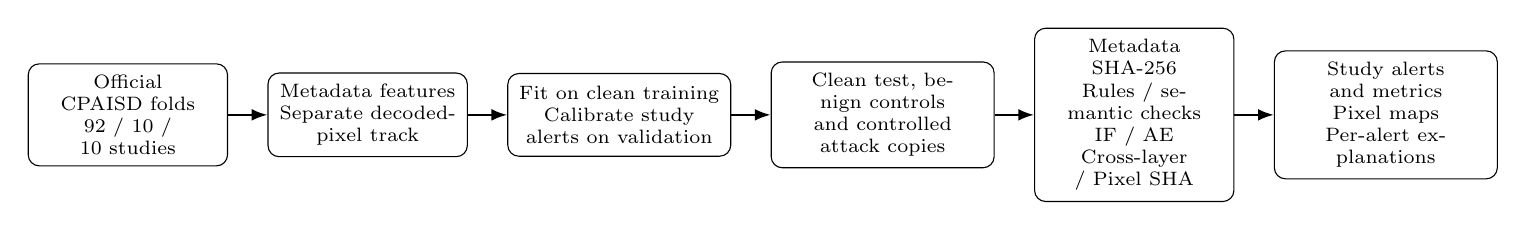
\begin{tikzpicture}[
    node distance=5mm,
    block/.style={draw,rounded corners,align=center,text width=2.25cm,minimum height=1.05cm,inner sep=4pt,font=\scriptsize},
    wide/.style={draw,rounded corners,align=center,text width=2.55cm,minimum height=1.05cm,inner sep=4pt,font=\scriptsize},
    arrow/.style={-{Latex[length=2mm]},thick}
  ]
  \node[block] (folds) {Official CPAISD folds\\92 / 10 / 10 studies};
  \node[block,right=of folds] (features) {Metadata features\\Separate decoded-pixel track};
  \node[wide,right=of features] (fit) {Fit on clean training\\Calibrate study alerts on validation};
  \node[wide,right=of fit] (test) {Clean test, benign controls\\and controlled attack copies};
  \node[block,right=of test] (detect) {Metadata SHA-256\\Rules / semantic checks\\IF / AE\\Cross-layer / Pixel SHA};
  \node[wide,right=of detect] (report) {Study alerts and metrics\\Pixel maps\\Per-alert explanations};
  \draw[arrow] (folds.east) -- (features.west);
  \draw[arrow] (features.east) -- (fit.west);
  \draw[arrow] (fit.east) -- (test.west);
  \draw[arrow] (test.east) -- (detect.west);
  \draw[arrow] (detect.east) -- (report.west);
  \end{tikzpicture}
  \caption{Research workflow with metadata and pixel tracks, reference-free layout checks, validation-calibrated study alerts, controlled edits, and per-alert explanations.}
  \label{fig:pipeline}
  \end{figure*}
  
  \subsection{Dataset and split}
  CPAISD contains 112 anonymized hyperacute ischemic-stroke NCCT studies. The official folds contain 92 training studies (8,376 DICOM instances), 10 validation studies (980 instances), and 10 test studies (809 instances) \cite{umerenkov2025}. The selector retained all studies in the three official folds and reported zero nonempty PatientID overlap across folds. In this run, the observed counts were 8,376, 980, and 809 readable files, respectively; all were reported as CT, with 92/10/10 unique studies and series. The metadata models use headers only and do not use stroke annotations. The separate pixel experiment decodes PixelData only for the 809 test instances and their synthetic copies.
  
  \subsection{Metadata representation}
  For each DICOM instance $x_i$, the implementation extracts numeric attributes (including rows, columns, bit depth, slice thickness, spacing between slices, rescale parameters, KVP, and tube current) and presence/length features for selected text fields (including PatientID, PatientName, StudyDescription, SeriesDescription, ProtocolName, Modality, Manufacturer, PhotometricInterpretation, and BodyPartExamined). Manufacturer, Modality, PhotometricInterpretation, and BodyPartExamined are also represented categorically. Patient identifiers and names are not retained as raw text in the feature vector; non-category text contributes only presence and length. In the inspected test fold, PatientID, PatientName, StudyDescription, and SeriesDescription were absent from all 809 files; ProtocolName and InstitutionName were present as ``Anonymized'' in all files, while Manufacturer had two values. Thus the PatientID and StudyDescription scripts in the original run inserted previously absent attributes rather than replacing existing identifiers or descriptions. Missing or nonnumeric values are mapped to defaults in the current implementation, which can conflate a genuine zero with a missing value.
  
  \subsection{Cryptographic comparator}
  The implementation recursively serializes main-dataset and file-meta (group 0002) DICOM elements by tag, converts values to strings, excludes PixelData (7FE0,0010) and group-length elements, and serializes the resulting mapping as sorted compact UTF-8 JSON. The SHA-256 digest for instance $i$ is
  \begin{equation}
  h_i = \mathrm{SHA256}(\mathrm{JSON}_{\mathrm{canonical}}(M_i)),
  \end{equation}
  where $M_i$ denotes the parsed metadata elements. A reference manifest maps each relative file path to a clean metadata digest and records SOP, Study, and Series Instance UIDs. Detection flags a mismatch if the path is absent from the manifest or the recalculated digest differs. This is a reference comparison, not a digital signature: the manifest must be protected independently, and this experiment creates it directly from the held-out clean test objects. Therefore, clean-control FPR for the hash comparator is zero by construction, and its perfect detection of file-level edits is expected. The manifest should be access-controlled because its DICOM UIDs remain linkable identifiers even though the image cohort is anonymized.

  \subsection{Authenticated manifest transfer prototype}
  To extend file-level integrity checks toward secure DICOM exchange, we implemented a sender--receiver workflow that stores a signed manifest as a sidecar to each DICOM object. The manifest records a schema version, unique manifest identifier, creation time, DICOM identifiers, and SHA-256 digests for canonical metadata, raw PixelData, and optionally the complete serialized file. Canonical metadata serialization includes nested sequences and file-meta elements while excluding PixelData; the raw-file digest covers the complete serialized object. The sender signs the canonical manifest representation with Ed25519. At the receiver, signature verification is checked against an explicit trusted-public-key registry before content hashes are compared. The verifier distinguishes a valid signature and matching content (VERIFIED), content mismatch, invalid signature, untrusted signer, and missing reference. An optional HMAC-SHA256 sidecar demonstrates shared-secret authentication; because any key holder can generate an HMAC, it does not provide individual signer attribution. An optional local replay cache flags a previously accepted manifest identifier for policy review.

  The integrated analysis workflow verifies the manifest first, then runs the project's existing structural rules, study/series consistency checks, metadata anomaly models, pixel anomaly model, and saved localization models on accepted content (Fig.~\ref{fig:signed_manifest_workflow}). Research-copy transformation is separated from verification: the prototype creates a limited pseudonymized copy and generates a fresh signature for that transformed object. Private-tag removal and selected metadata pseudonymization do not implement the complete DICOM PS3.15 confidentiality profile; pixel cleaning and workflow-specific requirements are outside this prototype \cite{dicomps315}. The implementation uses signed JSON sidecars rather than DICOM Digital Signatures and does not implement a live DICOM network transport association. It therefore demonstrates authenticated integrity at the sender--receiver application boundary, not protocol conformance or measured network performance.

  \begin{figure*}[t]
  \centering
  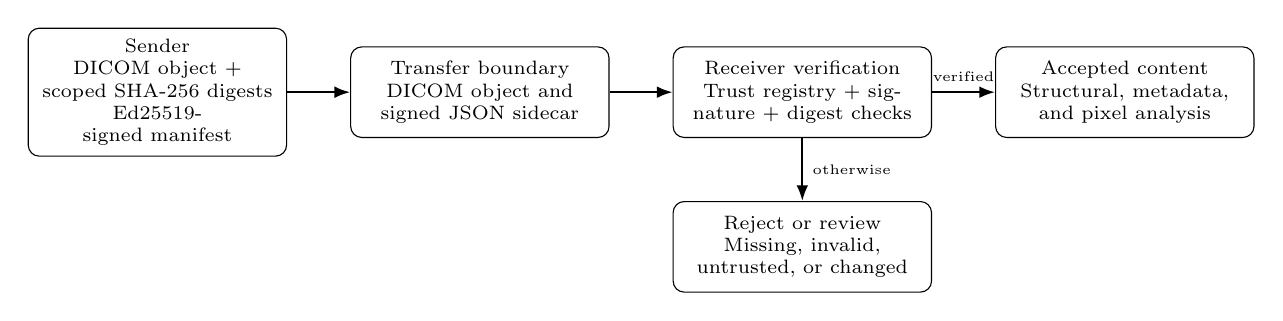
\begin{tikzpicture}[
    node distance=8mm,
    stage/.style={draw,rounded corners,align=center,text width=3.0cm,minimum height=1.15cm,inner sep=4pt,font=\scriptsize},
    arrow/.style={-{Latex[length=2mm]},thick}
  ]
  \node[stage] (sender) {Sender\\DICOM object + scoped SHA-256 digests\\Ed25519-signed manifest};
  \node[stage,right=of sender] (transfer) {Transfer boundary\\DICOM object and signed JSON sidecar};
  \node[stage,right=of transfer] (verify) {Receiver verification\\Trust registry + signature + digest checks};
  \node[stage,right=of verify] (analysis) {Accepted content\\Structural, metadata, and pixel analysis};
  \node[stage,below=of verify] (reject) {Reject or review\\Missing, invalid, untrusted, or changed};
  \draw[arrow] (sender.east) -- (transfer.west);
  \draw[arrow] (transfer.east) -- (verify.west);
  \draw[arrow] (verify.east) -- node[above,font=\tiny]{verified} (analysis.west);
  \draw[arrow] (verify.south) -- node[right,font=\tiny]{otherwise} (reject.north);
  \end{tikzpicture}
  \caption{Application-level signed-manifest workflow. The receiver checks signer trust and the signature before comparing DICOM digests and passing accepted objects to the existing detectors. This prototype does not implement a DICOM network association or measure transport performance.}
  \label{fig:signed_manifest_workflow}
  \end{figure*}
  
  \subsection{Structural rules}
  Rules flag missing required attributes (SOPClassUID, SOPInstanceUID, StudyInstanceUID, SeriesInstanceUID, Modality, Rows, Columns), non-CT modality, nonpositive image dimensions, invalid or nonpositive two-value PixelSpacing, nonpositive SliceThickness when present, and a SeriesInstanceUID associated with more than one StudyInstanceUID in the evaluated directory. The final rule is series-contextual: one inconsistent instance can cause other instances in its series to be flagged. The current attack log, however, marks only files actually edited as positives. This mismatch is material for the UID-inconsistency result and is discussed in Section~\ref{sec:limitations}.
  
  \subsection{Study/series metadata consistency}
  An additional interpretable checker tests whether selected metadata values agree among instances sharing a study or series identifier. At study level it compares PatientID, PatientName, PatientBirthDate, PatientSex, and StudyDate. At series level it compares StudyInstanceUID, Modality, Manufacturer, ProtocolName, Rows, Columns, SamplesPerPixel, PhotometricInterpretation, BitsAllocated, BitsStored, HighBit, PixelRepresentation, PixelSpacing, ImageOrientationPatient, and SliceThickness. It also checks the tag dependencies $\mathrm{HighBit}=\mathrm{BitsStored}-1$ and, for single-sample CT, a monochrome PhotometricInterpretation. A conflict is reported when present values disagree or a tag is present in some group members but absent in others; groups with fewer than two instances are not compared. Findings are attached to all members of a conflicting group, so metrics are aggregated by baseline-keyed study in the controlled experiment. A separate coordinated-edit condition changes ProtocolName to the same-length substituted value in every instance of each selected study, testing whether group checks detect a value that is wrong relative to the reference but internally consistent. These are consistency constraints, not clinical semantic validation: a coordinated edit that remains consistent across the group can evade them, and a conflict does not establish malicious intent.
  
  \subsection{Header-to-pixel layout consistency}
  A separate reference-free check compares pixel-layout declarations in the header with the pixel payload. It validates positive Rows, Columns, SamplesPerPixel, NumberOfFrames, and bit-depth fields; checks that uncompressed PixelData length agrees with declared dimensions; decodes PixelData and compares array shape with the header; and checks decoded values against the declared BitsStored and PixelRepresentation range. For compressed transfer syntaxes, the raw byte-length check is skipped while decoded shape and value checks remain. This detects structural contradictions between header and payload, not subtle semantic changes to otherwise valid pixels.
  
  \subsection{Isolation Forest}
  The Isolation Forest uses $300$ trees and is fit to the dense DictVectorizer output from clean training instances. It uses seed 42. Let $s_{\mathrm{IF}}(x)$ be the model's decision score, where lower values are more anomalous. Its cutoff is the first percentile of the 980 clean validation scores:
  \begin{equation}
  \tau_{\mathrm{IF}} = Q_{0.01}\left(\{s_{\mathrm{IF}}(x):x\in V\}\right), \quad
  \hat y_{\mathrm{IF}}(x)=\mathbb{1}[s_{\mathrm{IF}}(x)<\tau_{\mathrm{IF}}].
  \end{equation}
  This defines an instance-level nominal validation-tail rate, not a guaranteed 1\% study-level FPR; slices are clustered within studies.
  
  \subsection{Metadata autoencoder}
  The autoencoder uses a dense DictVectorizer and StandardScaler fit on clean training data. Its encoder has layer widths $d\rightarrow32\rightarrow16\rightarrow8\rightarrow4$ and its decoder mirrors these widths to reconstruct the $d$-dimensional input; hidden layers use ReLU activations. It is trained for 40 epochs with batch size 32, Adam at learning rate $10^{-3}$, and mean squared reconstruction loss. For standardized feature vector $z_i$, reconstruction error is
  \begin{equation}
  e_i = \frac{1}{d}\lVert z_i - f_{\theta}(z_i)\rVert_2^2.
  \end{equation}
  The classification threshold is the 99th percentile of clean validation errors, and an instance is anomalous when $e_i>\tau_{\mathrm{AE}}$. For the optimizer comparison, the architecture, 40-epoch budget, batch size (32), learning rate ($10^{-3}$), seed (42), training/validation folds, and threshold percentile were held fixed. Adam was the existing baseline; the alternatives were RMSprop, AdamW with weight decay $10^{-4}$, and SGD with momentum $0.9$. Each model was fitted on clean training data and calibrated independently on clean validation data. No optimizer-specific learning-rate search or repeated-seed averaging was performed.
  Reconstruction-objective comparisons instead used RMSprop for all models, 40 epochs, seed 42, and independent clean-validation thresholds. The denoising autoencoder was trained with Gaussian noise of standard deviation 0.1 and random feature masking probability 0.05, while reconstructing the original clean feature vector. Fixed mixed-loss and standard-MSE models used identical data and training budgets.
  
  Prediction records include the detector sources, structural-rule findings, anomaly scores and thresholds, and the autoencoder's highest feature-wise squared reconstruction errors. These contributions indicate which encoded dimensions contributed most to reconstruction loss; they are diagnostic associations, not causal explanations. A hash mismatch confirms a difference from its reference but cannot identify the changed tag.

  \subsection{Mixed reconstruction objectives and bilevel group weights}
  In addition to MSE, MAE, Smooth L1, log-cosh, and denoising objectives, we evaluated a mixed reconstruction loss for the heterogeneous metadata feature vector:
  \begin{equation}
  L_{\mathrm{mixed}}=w_nL_{\mathrm{Huber}}+w_cL_{\mathrm{CE}}+w_pL_{\mathrm{BCE}},\qquad
  w_n+w_c+w_p=1,\quad w_g\geq0.
  \end{equation}
  Numerical feature groups use Smooth L1 (Huber) loss, categorical groups use cross-entropy, and binary tag-presence indicators use binary cross-entropy. A fixed mixed baseline assigns one-third weight to each group. In the bilevel variant, the autoencoder parameters are optimized by RMSprop, while Adam updates three loss-weight logits through a softmax parameterization. Each epoch uses a one-step differentiable SGD proxy update to estimate a hypergradient for a validation ranking objective: scores for synthetic edits should exceed scores for their clean counterparts by a margin. The outer optimizer uses learning rate $10^{-2}$ and the inner proxy step size is $10^{-3}$. Five validation studies supply in-memory synthetic edit pairs for weight updates; five disjoint clean studies calibrate the final score threshold. This is a one-step truncated hypergradient approximation, not exact bilevel convergence.

  A separate fixed-weight sweep compared plain MSE, MSE with both PixelSpacing feature errors weighted by 2, and nine mixed-loss triples. Each of the 11 settings was trained with RMSprop for 40 epochs under seeds 42, 43, and 44. Within each seed, five validation studies set the threshold at the 98th percentile of clean file scores, and five disjoint studies evaluated the clean false-alarm rate and synthetic attack recall. A setting met the target only if its held-out validation file FPR was at most 2\%. Test-fold metrics were not used for selection. This protocol is distinct from the single-seed bilevel experiment above.
  
  \subsection{Controlled modifications and hybrid decision}
  The original metadata run generated six attack variants on copies of the clean test directory. For each type, 20\% of test studies (2 of 10) were selected with seed 42; because the same seed and ordered input were used, the same two studies were selected across attack variants. The PatientID and StudyDescription conditions inserted those absent attributes; PixelSpacing values were multiplied by 1.7; ProtocolName was removed when present; and Modality was changed from CT to MR. The first five conditions each produced 177 changed files. The UID-inconsistency variant changed one instance per selected series, or two instances total. Its file-level ground truth marks only those two files positive. A subsequent extension added two same-length substitutions on fields that are populated in CPAISD: a deterministic character substitution in ProtocolName (10 characters) and Manufacturer (7 or 18 characters), each preserving the original string length and producing 177 modified files.
  
  The adaptive-evasion experiment gives the attacker knowledge of the feature map and selects a same-length ProtocolName substitution. The feature extractor records ProtocolName presence and length but not its content, so the experiment measures an explicit feature-collision attack against learned detectors while retaining the trusted-reference hash as a control. This is a white-box feature-map evasion test, not optimization over arbitrary fields or unknown detector architectures.
  
  Let $m_i$, $r_i$, $u_i$, and $a_i$ be the hash, rule, Isolation Forest, and autoencoder binary outputs. The hybrid decision is
  \begin{equation}
  \hat y_{\mathrm{H}}(x_i)=m_i\lor r_i\lor u_i\lor a_i.
  \end{equation}
  An OR rule ensures the hybrid includes any detection from a component, but cannot be expected to improve over a perfect reference hash in this threat model and can increase false alarms.
  
  \subsection{Separate pixel-integrity experiment}
  The pixel experiment uses the clean 809-instance test fold and creates a second copy for each of three deterministic, pixel-only conditions. For each attack, the same seed (42) selects 20\% of the ten studies (two studies). The localized-patch condition adds 32 to a central $5\times5$ patch in each slice of the selected studies (177 files). The low-amplitude condition adds 1 to a seeded random 1\% of stored pixel values in each selected slice (177 files). The slice-inconsistency condition adds 8 to a central $5\times5$ patch in one sorted slice per selected series (two files in this cohort). Modifications are applied to copies; original CPAISD files are not edited. Values are changed in the stored integer domain without applying RescaleSlope or RescaleIntercept, so the parameters are not expressed as Hounsfield-unit changes.
  
  For clean pixel array $P_i$ and its edited copy $P_i'$, the pointwise difference map is
  \begin{equation}
  D_i(u,v)=\left|P_i'(u,v)-P_i(u,v)\right|.
  \end{equation}
  The implementation records the changed-pixel count and fraction, mean absolute difference (MAE), root-mean-square difference (RMSE), and maximum absolute difference. Representative figures show the clean slice, modified slice, and $D_i$; the difference image is scaled per example for visibility. Packed binary masks record the pixels actually changed by each synthetic edit. For a descriptive alignment check, the mask is compared with the reference-derived map $\mathbb{1}[D_i(u,v)>0]$. Because this thresholded map is computed from the exact same clean/edited pair, its overlap is a procedural consistency check, not a detector's localization performance. The integrity comparator computes SHA-256 over raw DICOM PixelData and compares it with a per-file clean-test digest. Metadata SHA-256, which excludes PixelData, serves as a negative control. The no-reference anomaly baseline is evaluated separately below.
  
  \subsection{No-reference pixel anomaly baseline}
  The no-reference detector operates on each image independently and never reads a clean counterpart or a pixel hash during prediction. Each image is robustly scaled using its 1st and 99th intensity percentiles, partitioned into non-overlapping $16\times16$ patches, and represented by six local intensity/texture features: mean, standard deviation, horizontal and vertical mean absolute gradients, high-deviation fraction, and log-scaled standard deviation. An Isolation Forest with 100 trees is fit to 50,000 randomly sampled clean patches from 2,084 training slices. Two thresholds are calibrated on clean validation data: the 1st percentile of validation patch scores for pixel-map blocks, and the 1st percentile of per-image minimum patch scores for image alarms. The saved synthetic masks are used only for evaluation. Predicted localization is blockwise at $16\times16$ resolution, so localization metrics reflect this coarse grid and the specified synthetic attacks.
  
  A second no-reference comparator computes a $5\times5$ median-filter residual $R_i=|I_i-\operatorname{MedianFilter}_{5\times5}(I_i)|$ on each independently normalized image. Its pixel threshold is the 99.9th percentile of clean validation residual samples. Its image alarm score is the 99.9th percentile residual within an image, thresholded at the 99th percentile of these image scores on clean validation data. This comparator is a simple high-frequency baseline; neither its prediction nor calibration uses a clean test counterpart.
  
  \subsection{Supervised U-Net localization model}
  The supervised pixel baseline is a compact 2-D U-Net with four encoder stages, a bottleneck, four decoder stages, and skip concatenations following the standard U-Net design \cite{ronneberger2015}. Each stage uses two $3\times3$ convolutions with batch normalization and ReLU; encoder stages are separated by $2\times2$ max pooling, and decoder stages use $2\times2$ transposed convolutions. With base width $b=8$, the feature widths are $8,16,32,64,128$ from input to bottleneck, then $64,32,16,8$ through the decoder. A $1\times1$ convolution produces one per-pixel logit map. Each input is robustly normalized using its 1st and 99th intensity percentiles and resized to $256\times256$; inference uses the image alone, without a clean counterpart or hash.

  An Attention U-Net comparator retains the same encoder, decoder, widths, losses, optimizer, folds, and validation-based checkpoint selection, but adds attention gates to weight each encoder skip feature map using the corresponding decoder context. Fig.~\ref{fig:attention_gate} details the gate inserted at each of the four skip connections in Fig.~\ref{fig:unet_architecture}. This is an architecture ablation, not an assumption that attention necessarily improves localization or adversarial robustness.
  
  Training uses synthetic localized patches and sparse low-amplitude perturbations, with the exact changed pixels serving as binary supervision masks. The network is trained with a weighted binary-cross-entropy and soft-Dice objective, each weighted by $0.5$, using AdamW (learning rate $10^{-3}$, weight decay $10^{-4}$). The positive BCE weight is 12 to account for the small edited area. Clean validation predictions set the pixel threshold to the 99.5th percentile of sampled pixel probabilities and the image threshold to the 99th percentile of per-image maximum probabilities. A copy-move family is withheld from training and used as a synthetic out-of-family test. The model grid and masks are resized representations; no native-resolution clinical annotation is used.

  \subsection{Targeted FGSM and PGD evasion evaluation}
  A separate robustness experiment evaluates the trained U-Net without retraining. For each selected synthetic test edit, FGSM applies one gradient-sign step and PGD applies ten iterative steps to the normalized image array. Both use an $L_\infty$ budget $\epsilon=0.02$ in the $[0,1]$ normalized input domain; PGD uses step size 0.004 and a seeded random start. The targeted objective minimizes binary cross-entropy against an all-clean mask to suppress the predicted tamper response. Adversarial variants are generated in memory and do not overwrite DICOM files. The validation-calibrated image and pixel thresholds are held fixed. Attack success rate is the fraction of images detected before perturbation that fall below the fixed image alarm threshold afterward. Localization is measured against the original synthetic edit mask. This tests evasion of this particular U-Net on these scripted edits; it is not a real-world clinical attack, and an exact-reference PixelData hash would still detect a serialized pixel change.
  
  The initial four-epoch pilot reported below used its final epoch. The revised runner additionally generates fixed localized-patch and sparse-edit masks on a 256-image validation subset (128 images per family), computes family-wise pixel Dice and IoU after each epoch at probability threshold 0.5, and selects the checkpoint with the best macro validation IoU. In the 30-epoch run, epoch 30 was selected; the final test evaluation completed using this checkpoint.
  
  \begin{figure*}[t]
  \centering
  \resizebox{\textwidth}{!}{%
  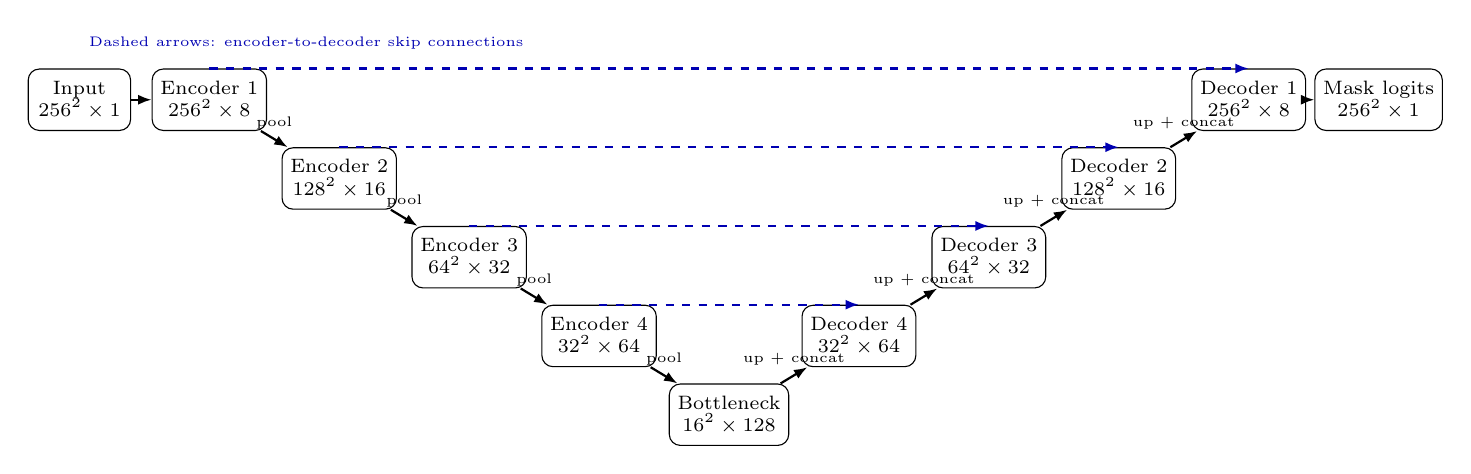
\begin{tikzpicture}[
    block/.style={draw,rounded corners,align=center,minimum width=1.30cm,minimum height=0.78cm,inner sep=3pt,font=\scriptsize},
    arrow/.style={-{Latex[length=1.7mm]},thick},
    skip/.style={-{Latex[length=1.7mm]},thick,dashed,blue!70!black}
  ]
  \node[block] (input) at (0,0) {Input\\$256^2\times1$};
  \node[block] (enc1) at (1.65,0) {Encoder 1\\$256^2\times8$};
  \node[block] (enc2) at (3.30,-1) {Encoder 2\\$128^2\times16$};
  \node[block] (enc3) at (4.95,-2) {Encoder 3\\$64^2\times32$};
  \node[block] (enc4) at (6.60,-3) {Encoder 4\\$32^2\times64$};
  \node[block] (bottleneck) at (8.25,-4) {Bottleneck\\$16^2\times128$};
  \node[block] (dec4) at (9.90,-3) {Decoder 4\\$32^2\times64$};
  \node[block] (dec3) at (11.55,-2) {Decoder 3\\$64^2\times32$};
  \node[block] (dec2) at (13.20,-1) {Decoder 2\\$128^2\times16$};
  \node[block] (dec1) at (14.85,0) {Decoder 1\\$256^2\times8$};
  \node[block] (output) at (16.50,0) {Mask logits\\$256^2\times1$};
  \draw[arrow] (input) -- (enc1);
  \draw[arrow] (enc1) -- node[above,font=\tiny]{pool} (enc2);
  \draw[arrow] (enc2) -- node[above,font=\tiny]{pool} (enc3);
  \draw[arrow] (enc3) -- node[above,font=\tiny]{pool} (enc4);
  \draw[arrow] (enc4) -- node[above,font=\tiny]{pool} (bottleneck);
  \draw[arrow] (bottleneck) -- node[above,font=\tiny]{up + concat} (dec4);
  \draw[arrow] (dec4) -- node[above,font=\tiny]{up + concat} (dec3);
  \draw[arrow] (dec3) -- node[above,font=\tiny]{up + concat} (dec2);
  \draw[arrow] (dec2) -- node[above,font=\tiny]{up + concat} (dec1);
  \draw[arrow] (dec1) -- (output);
  \draw[skip] (enc4.north) -- (dec4.north);
  \draw[skip] (enc3.north) -- (dec3.north);
  \draw[skip] (enc2.north) -- (dec2.north);
  \draw[skip] (enc1.north) -- (dec1.north);
  \node[font=\tiny,blue!70!black,anchor=west] at (0.0,0.72) {Dashed arrows: encoder-to-decoder skip connections};
  \end{tikzpicture}%
  }
  \caption{Implemented compact U-Net used for synthetic pixel-tamper localization. Convolutional blocks contain two $3\times3$ convolution, batch-normalization, and ReLU layers. Decoder stages upsample and concatenate the corresponding encoder features; the output is a per-pixel logit map.}
  \label{fig:unet_architecture}
  \end{figure*}

  \begin{figure*}[t]
  \centering
  \resizebox{0.98\textwidth}{!}{%
  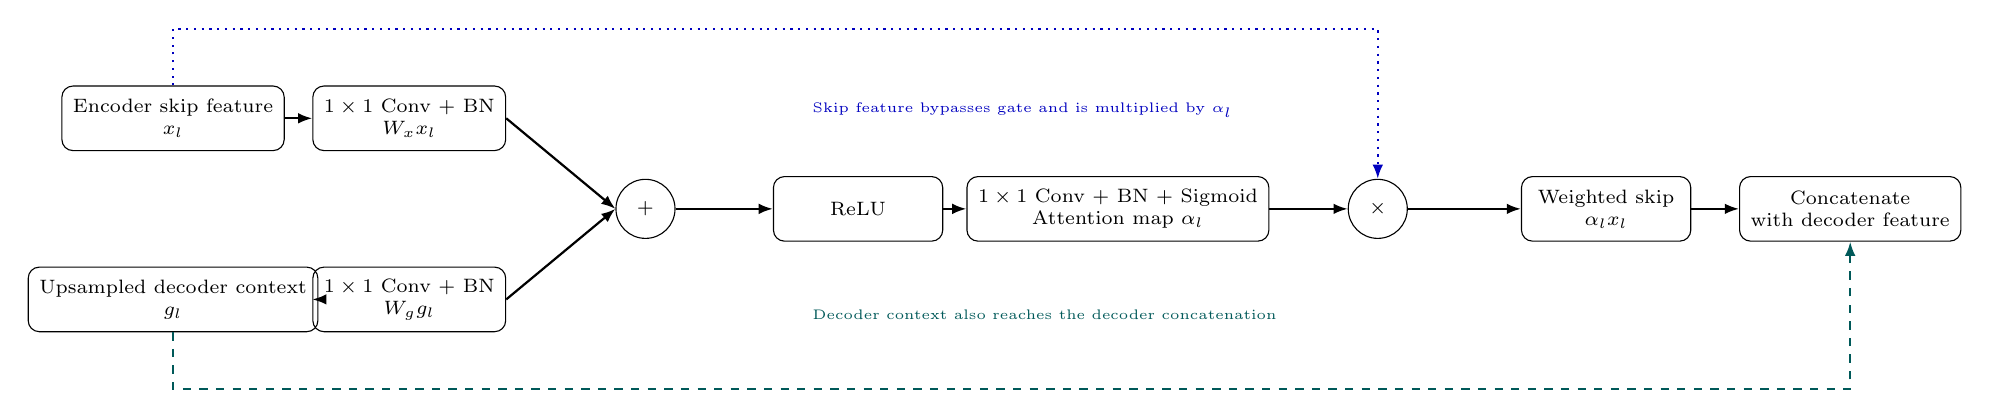
\begin{tikzpicture}[
    box/.style={draw,rounded corners,align=center,minimum width=2.15cm,minimum height=0.82cm,inner sep=4pt,font=\scriptsize},
    op/.style={draw,circle,align=center,minimum size=0.75cm,inner sep=1pt,font=\scriptsize},
    flow/.style={-{Latex[length=1.8mm]},thick},
    context/.style={-{Latex[length=1.8mm]},thick,dashed,teal!70!black},
    bypass/.style={-{Latex[length=1.8mm]},thick,dotted,blue!75!black}
  ]
  \node[box] (skip) at (0,1.15) {Encoder skip feature\\$x_l$};
  \node[box] (decoder) at (0,-1.15) {Upsampled decoder context\\$g_l$};
  \node[box] (projx) at (3.0,1.15) {$1\times1$ Conv + BN\\$W_x x_l$};
  \node[box] (projg) at (3.0,-1.15) {$1\times1$ Conv + BN\\$W_g g_l$};
  \node[op] (sum) at (6.0,0) {$+$};
  \node[box] (relu) at (8.7,0) {ReLU};
  \node[box] (attention) at (12.0,0) {$1\times1$ Conv + BN + Sigmoid\\Attention map $\alpha_l$};
  \node[op] (multiply) at (15.3,0) {$\times$};
  \node[box] (weighted) at (18.2,0) {Weighted skip\\$\alpha_l x_l$};
  \node[box] (concat) at (21.3,0) {Concatenate\\with decoder feature};
  \draw[flow] (skip.east) -- (projx.west);
  \draw[flow] (decoder.east) -- (projg.west);
  \draw[flow] (projx.east) -- (sum.west);
  \draw[flow] (projg.east) -- (sum.west);
  \draw[flow] (sum.east) -- (relu.west);
  \draw[flow] (relu.east) -- (attention.west);
  \draw[flow] (attention.east) -- (multiply.west);
  \draw[flow] (multiply.east) -- (weighted.west);
  \draw[flow] (weighted.east) -- (concat.west);
  \draw[bypass] (skip.north) -- ++(0,0.72) -| (multiply.north);
  \draw[context] (decoder.south) -- ++(0,-0.72) -| (concat.south);
  \node[font=\tiny,blue!75!black,anchor=west] at (8.0,1.25) {Skip feature bypasses gate and is multiplied by $\alpha_l$};
  \node[font=\tiny,teal!70!black,anchor=west] at (8.0,-1.35) {Decoder context also reaches the decoder concatenation};
  \end{tikzpicture}%
  }
  \caption{Attention gate used at each Attention U-Net skip connection. Encoder features and upsampled decoder context are projected, combined, and passed through a sigmoid to form a spatial attention map. The map weights the encoder skip before concatenation with the decoder feature. The encoder-decoder stages are otherwise those shown in Fig.~\ref{fig:unet_architecture}.}
  \label{fig:attention_gate}
  \end{figure*}
  
  \subsection{Study-level conformal calibration}
  To calibrate alerts at the unit of use, slice scores are aggregated per baseline-keyed study using maximum anomaly severity: $-s_{\mathrm{IF}}$ for Isolation Forest and reconstruction error for the autoencoder. For a test-study score $q$, the conformal tail probability is
  \begin{equation}
  p(q)=\frac{1+\sum_{j=1}^{n_v}\mathbb{1}[q_j^{(v)}\ge q]}{n_v+1},
  \end{equation}
  where $q_j^{(v)}$ are clean validation-study scores. An alert is emitted when $p(q)\le\alpha$. With ten validation studies, the smallest attainable $p$-value is $1/11\approx0.091$; nominal levels below this cannot emit an alert under this calibration.
  
  \subsection{Severity sweep and combined conditions}
  The severity sweep uses three predefined settings. The subtle setting applies a $3\times3$ patch with increment 1, a seeded 0.1\% sparse perturbation with increment 1, and the same patch operation to one slice per selected series. The default setting uses the primary attack parameters described above. The stronger setting uses a $9\times9$ patch with increment 32, a seeded 5\% sparse perturbation with increment 2, and a $9\times9$ slice patch with increment 32. These increments apply to stored integer values, not HU.
  
  Four combined conditions pair PatientID insertion or Modality metadata edits with localized-patch or low-amplitude pixel edits. In the initial run, both generators used seed 42 and selected the same two studies, so the two hash checks each covered the full positive set. A corrected rerun used seed 42 for metadata selection and seed 44 for pixel selection; the selected study pairs were disjoint. This produced metadata-only, pixel-only, and union-positive files. Metadata and pixel SHA-256 are scored separately against the original clean test reference, and their OR is reported as a reference-based combined comparator. This does not test learned fusion or performance without a trusted reference. An external-evaluation script is also provided for CPAISD-trained metadata models on a separately acquired DICOM cohort; no external cohort results are reported because such a dataset was not present for this run.
  
  \subsection{Evaluation protocol}
  Models were fit using clean training data only. Thresholds were chosen from clean validation data only. A metadata baseline was generated for each clean test file, then used for clean-control evaluation and for all attacked copies. The attack log supplied file-level labels. For each attack and method, accuracy, precision, recall, F1, specificity, false-positive rate, and confusion counts were computed. The original six-condition macro averages give each of those attack conditions equal weight; the two later same-length experiments are reported separately and are not included in those macro results. Clean-test false-positive rates were computed separately at file and study level. A seed-sensitivity extension repeats four representative attacks with seeds 42, 43, and 44. It reports per-run results and 2,000-resample percentile bootstrap intervals, resampling the immutable baseline-keyed study (or series) as the cluster. These intervals describe only the ten-study test fold and are not external-population uncertainty estimates.
  
  \begin{table}[t]
  \caption{Metrics used in the experiment.}
  \label{tab:metrics}
  \centering\footnotesize
  \begin{tabular}{ll}
  \toprule
  Metric & Definition \\
  \midrule
  Precision & $TP/(TP+FP)$ \\
  Recall & $TP/(TP+FN)$ \\
  F1 & $2PR/(P+R)$ \\
  Specificity & $TN/(TN+FP)$ \\
  FPR & $FP/(FP+TN)=1-\mathrm{specificity}$ \\
  \bottomrule
  \end{tabular}
  \end{table}
  
  \section{Results and Experiments}
  \subsection{Dataset description}
  The full official CPAISD folds were used: 92 train studies/8,376 files, 10 validation studies/980 files, and 10 test studies/809 files. Metadata inspection found only Modality=CT in each fold, and the number of unique series equaled the number of studies. All 809 clean test instances were retained for each of six original metadata attack conditions. Five attack variants produced 177 positives each; the UID-inconsistency variant produced two file-level positives. Thus the six original condition tables contain $6\times809=4,854$ file-condition observations and 887 positive file labels. The two additional same-length conditions each contain 809 observations and 177 positives. These are repeated test files under different attack conditions, not independent patients or studies.

  \subsection{Signed-manifest security evaluation}
  We evaluated the sender--receiver security prototype on all 809 readable test-fold DICOM files. For each object, an experiment-only Ed25519 key signed a sidecar manifest; a local trust registry represented receiver trust. The test runner applied 13 scenarios to temporary copies or manifest objects, including content edits, signature and trust failures, an incorrect HMAC key, replay-cache behavior, a forged unsigned digest reference, preamble-only reserialization, and authorized research-copy de-identification followed by re-signing. For the one-pixel scenario, decoded arrays were compared after serialization and each supported object was required to differ at exactly one pixel. The reserialization test changed the 128-byte PS3.10 preamble while keeping parsed metadata and PixelData equal. It was checked under both a raw-file-scoped manifest and a content-only manifest. Original CPAISD files were not modified.

  \begin{table*}[t]
  \caption{Signed-manifest security scenarios on the CPAISD test fold. Each scenario was evaluated on 809 files; outcomes are verifier status unless noted.}
  \label{tab:signed_manifest_scenarios}
  \centering\scriptsize
  \begin{tabular}{p{5.1cm}p{4.0cm}p{6.2cm}}
  \toprule
  Scenario & Observed outcome & Interpretation \\
  \midrule
  Unchanged signed object & VERIFIED (809/809) & Signature trusted and all signed digest scopes matched. \\
  Metadata edit & INTEGRITY\_MISMATCH (809/809) & Signed metadata digest differed from the received object. \\
  Pixel-byte flip & INTEGRITY\_MISMATCH (809/809) & PixelData digest differed. \\
  Single decoded-pixel edit & INTEGRITY\_MISMATCH (809/809) & Exactly one decoded value changed in each test object. \\
  Forged unsigned digest reference & UNSIGNED\_REFERENCE\_ACCEPTS (809/809) & Digest-only comparison accepted the attacker's own reference; no signer authentication was present. \\
  Altered manifest digest; forged signature & INVALID\_SIGNATURE (809/809 each) & Manifest signature validation failed. \\
  Untrusted signer & UNTRUSTED\_SIGNER (809/809) & Signer key was absent from the receiver trust registry. \\
  Missing signed reference & MISSING\_REFERENCE (809/809) & No signed manifest was provided. \\
  Incorrect HMAC key & INVALID (809/809) & Shared-secret tag validation failed. \\
  Preamble-only reserialization & INTEGRITY\_MISMATCH (809/809) & Raw-file-scoped digest detected changed bytes; the separate content-only manifest remained VERIFIED (809/809). \\
  Replayed manifest identifier & POLICY\_REVIEW\_REQUIRED (809/809) & Local replay cache recognized a previously accepted manifest. \\
  Authorized de-identify and re-sign & VERIFIED (809/809) & Transformed research copy matched its newly signed manifest. \\
  \bottomrule
  \end{tabular}
  \end{table*}

  The full run generated 10,517 file-scenario observations (13 scenarios per file). Mean manifest creation and signing time was 15.44 ms/file, and mean end-to-end verification time was 12.82 ms/file. The signed envelope averaged 868.4 bytes, corresponding to 0.1647\% of the serialized DICOM file size. These are local prototype measurements: no network transfer, association negotiation, throughput, packet loss, or concurrent workload was measured.

  \begin{table}[t]
  \caption{Local signed-manifest operation measurements across 809 test objects.}
  \label{tab:security_timing}
  \centering\footnotesize
  \begin{tabular}{lr}
  \toprule
  Measure & Mean \\
  \midrule
  Manifest creation and Ed25519 signing & 15.44 ms/file \\
  End-to-end verification & 12.82 ms/file \\
  Ed25519 signature operation & 0.147 ms/sign; 0.268 ms/verify \\
  Signed envelope size & 868.4 bytes \\
  Envelope / DICOM file size & 0.1647\% \\
  \bottomrule
  \end{tabular}
  \end{table}
  
  \subsection{Ablation and quantitative results}
  Table~\ref{tab:macro} gives the report's unweighted macro-average across six attack types at instance level. SHA-256 is perfect under the per-file reference setup. Among learned methods, the autoencoder has higher macro F1 than Isolation Forest (0.506 versus 0.116), but with a clean-test file FPR of 0.138. The hybrid reaches macro recall 1.000 and macro F1 0.635, while its FPR rises to 0.207. This is not evidence that the OR fusion is superior to a trusted hash: the hash component itself is expected to detect every changed metadata instance, and the OR rule inherits autoencoder false positives.
  
  \begin{table}[t]
  \caption{Macro-averaged instance-level results across the six attack types. Values are from the generated report; each attack type receives equal weight.}
  \label{tab:macro}
  \centering\footnotesize
  \begin{tabular}{lrrrrr}
  \toprule
  Method & Acc. & Prec. & Rec. & F1 & FPR \\
  \midrule
  SHA-256 reference & 1.000 & 1.000 & 1.000 & 1.000 & 0.000 \\
  Structural rules & 0.818 & 0.169 & 0.333 & 0.170 & 0.036 \\
  Isolation Forest & 0.837 & 0.167 & 0.089 & 0.116 & 0.000 \\
  Autoencoder & 0.825 & 0.408 & 0.667 & 0.506 & 0.171 \\
  IF + autoencoder & 0.825 & 0.408 & 0.667 & 0.506 & 0.171 \\
  Rules + IF & 0.838 & 0.335 & 0.423 & 0.287 & 0.036 \\
  OR hybrid & 0.826 & 0.512 & 1.000 & 0.635 & 0.207 \\
  \bottomrule
  \end{tabular}
  \end{table}
  
  The macro-average obscures substantial variation by attack. Table~\ref{tab:attack} reports per-attack recall and FPR for the principal comparators. Rule-based validation detected the Modality-to-MR edit, but not the PatientID, StudyDescription, PixelSpacing, or ProtocolName edits. Isolation Forest detected 53.7\% of PixelSpacing file edits and no PatientID, description, protocol, or modality edits. The autoencoder detected all file edits for four of the five whole-study attack types, but did not detect the modality edit and produced false alarms on clean files. Hash comparison detected all edited files, as expected under the constructed reference protocol.
  
  The original PatientID and StudyDescription conditions should be interpreted as insertion attacks because these tags were missing throughout the test fold. To probe whether feature length alone explains anomaly-model response, two additional same-length substitutions were run using populated fields. For both conditions the autoencoder retained its 17.72\% observed FPR on unmodified files; it detected all 177 Manufacturer substitutions but none of the 177 ProtocolName substitutions. Structural rules and Isolation Forest detected neither. These outcomes are descriptive for the chosen deterministic substitutions and do not establish robustness to other plausible edits.
  
  \begin{table}[t]
  \caption{Additional same-length metadata substitution results at file level. Entries are recall/FPR.}
  \label{tab:samelength}
  \centering\footnotesize
  \begin{tabular}{lrrrr}
  \toprule
  Attack & $n_+$ & SHA-256 & Isolation Forest & Autoencoder \\
  \midrule
  ProtocolName substitution & 177 & 1.00/0.00 & 0.00/0.00 & 0.00/0.177 \\
  Manufacturer substitution & 177 & 1.00/0.00 & 0.00/0.00 & 1.00/0.177 \\
  \bottomrule
  \end{tabular}
  \end{table}
  
  \subsection{Study-level semantic consistency experiment}
  The checker was evaluated on all 809 clean test instances grouped into ten baseline-keyed studies. It produced no findings on the clean fold. Six synthetic conditions then changed one instance in each of two selected studies: PatientID insertion/substitution, same-length ProtocolName and Manufacturer substitutions, a HighBit dependency violation, and UID/modality inconsistency positive controls. At the study unit, semantic consistency detected 2/2 affected studies with 0/8 false-positive studies for each condition. Existing structural rules also detected the UID and modality controls, but did not detect the first four conditions. As the semantic checker reports group conflicts on peer slices, it marked 151--177 instances per condition even though only two instances were edited; these instance counts are not file-level precision estimates. The dataset had only ten studies, and PatientID was absent from the original fold, so that condition is an insertion inconsistency rather than an altered existing identifier.
  
  \begin{table*}[t]
  \caption{Study-level structural and semantic consistency results for six one-instance-per-study synthetic edits. Each condition had two positive and eight negative studies. Entries are recall/FPR; semantic flags are propagated to members of the conflicting study/series.}
  \label{tab:semantic}
  \centering\footnotesize
  \begin{tabular}{lrrr}
  \toprule
  Condition & Structural rules & Semantic consistency & Semantic flagged instances \\
  \midrule
  PatientID insertion/substitution & 0.00/0.00 & 1.00/0.00 & 177 \\
  ProtocolName same-length change & 0.00/0.00 & 1.00/0.00 & 166 \\
  Manufacturer same-length change & 0.00/0.00 & 1.00/0.00 & 151 \\
  HighBit dependency violation & 0.00/0.00 & 1.00/0.00 & 177 \\
  Study UID inconsistency (positive control) & 1.00/0.00 & 1.00/0.00 & 173 \\
  Modality inconsistency (positive control) & 1.00/0.00 & 1.00/0.00 & 177 \\
  \bottomrule
  \end{tabular}
  \end{table*}

  \subsection{Coordinated study-wide metadata edit}
  To test the consistency checker's limit, the same-length ProtocolName substitution was applied either to one randomly selected instance in each of two studies or to every instance in those same two studies (177 instances total in the coordinated condition). Original DICOM files were read only; edits were evaluated on in-memory copies. Study-level labels were used because the attack unit was the study. The clean-reference metadata SHA-256 comparator was included alongside semantic and structural checks.

  \begin{table}[t]
  \caption{Study-level detection of slice-local versus coordinated ProtocolName edits (10 test studies; two positive studies per condition).}
  \label{tab:coordinated}
  \centering\scriptsize
  \begin{tabular}{llrrr}
  \toprule
  Condition & Detector & Recall & FPR & TP/FN \\
  \midrule
  One instance per study & Semantic consistency & 1.000 & 0.000 & 2/0 \\
  One instance per study & Structural rules & 0.000 & 0.000 & 0/2 \\
  One instance per study & Metadata SHA-256 reference & 1.000 & 0.000 & 2/0 \\
  Every instance in study & Semantic consistency & 0.000 & 0.000 & 0/2 \\
  Every instance in study & Structural rules & 0.000 & 0.000 & 0/2 \\
  Every instance in study & Metadata SHA-256 reference & 1.000 & 0.000 & 2/0 \\
  \bottomrule
  \end{tabular}
  \end{table}

  The semantic checker detected both studies when one instance was changed, because its ProtocolName disagreed with peer instances. It detected neither study after all instances were changed consistently. The reference hash detected both conditions because all edited metadata differed from the exact clean files. This is the expected distinction between internal-consistency checking and reference-based integrity verification; it is not evidence that either synthetic condition occurred in clinical practice.
  
  \subsection{Feature-aware adaptive evasion}
  In the feature-aware attack, 177 ProtocolName values were changed while preserving string length. The feature vectors were exactly unchanged for all 177 modified files. Metadata SHA-256 detected 177/177 changes; structural rules, Isolation Forest, and the autoencoder detected 0/177 each. The Isolation Forest score and autoencoder reconstruction error changed by exactly zero on average, and all three non-hash detectors were evaded on every modified file. This is a direct consequence of omitting ProtocolName content from the engineered feature map, rather than evidence of a novel attack optimizer. It demonstrates a concrete blind spot in this configuration: unsupervised models cannot detect information discarded before model input.
  
  \subsection{Header-to-pixel layout consistency}
  The reference-free layout checker produced no findings on the 809 clean test files. It flagged all 177 files in the Rows mismatch condition and all 177 in the Columns mismatch condition, with no false positives. The findings were the expected PixelData-length contradiction and pixel-decoding failure. It also flagged none of the 809 pixel-only low-amplitude negative-control files, which preserve declared dimensions and payload layout.
  
  \begin{table}[t]
  \caption{Header-to-pixel layout consistency results. Pixel-only edits are a negative control because their declared layout remains consistent.}
  \label{tab:crosslayer}
  \centering\scriptsize
  \begin{tabular}{lrrrr}
  \toprule
  Condition & Files & Positive files & Recall & FPR \\
  \midrule
  Clean control & 809 & 0 & -- & 0.000 \\
  Rows declared $+1$ & 809 & 177 & 1.000 & 0.000 \\
  Columns declared $+1$ & 809 & 177 & 1.000 & 0.000 \\
  Pixel-only negative control & 809 & 0 & -- & 0.000 \\
  \bottomrule
  \end{tabular}
  \end{table}
  
  These are clear but deliberately obvious layout contradictions. They do not show that the checker can identify plausible but incorrect metadata values that remain compatible with the encoded payload.
  
  \begin{table*}[t]
  \caption{Per-attack instance-level recall / FPR. $^{\dagger}$ In the UID-inconsistency condition, only edited files are labeled positive while the structural rule operates at series level; see Section~\ref{sec:limitations}.}
  \label{tab:attack}
  \centering\scriptsize
  \setlength{\tabcolsep}{6pt}
  \begin{tabular}{lrrrrrrr}
  \toprule
  Attack & $n_+$ & SHA-256 & Rules & IF & AE & OR hybrid \\
  \midrule
  PatientID & 177 & 1.00/0.00 & 0.00/0.00 & 0.00/0.00 & 1.00/0.18 & 1.00/0.18 \\
  Study description & 177 & 1.00/0.00 & 0.00/0.00 & 0.00/0.00 & 1.00/0.18 & 1.00/0.18 \\
  Pixel spacing & 177 & 1.00/0.00 & 0.00/0.00 & 0.54/0.00 & 1.00/0.18 & 1.00/0.18 \\
  UID inconsistency$^{\dagger}$ & 2 & 1.00/0.00 & 1.00/0.22 & 0.00/0.00 & 0.00/0.14 & 1.00/0.36 \\
  Protocol removal & 177 & 1.00/0.00 & 0.00/0.00 & 0.00/0.00 & 1.00/0.18 & 1.00/0.18 \\
  Modality change & 177 & 1.00/0.00 & 1.00/0.00 & 0.00/0.00 & 0.00/0.18 & 1.00/0.18 \\
  \bottomrule
  \end{tabular}\\
  \end{table*}
  
  \subsection{Series-level UID evaluation}
  The UID inconsistency attack changes one instance in each of two selected series. When predictions and labels are aggregated at the series level using the immutable clean baseline SeriesInstanceUID, the rule detector identifies both affected series with no false-positive series (recall 1.000, FPR 0.000). At file level, the same contextual rule flags 177 neighboring/affected instances while only two edited files are labeled positive, yielding 175 label-granularity false positives. The series-level result is the appropriate unit for this event; it still reflects a synthetic rule violation in a ten-series test fold.
  
  \begin{table}[t]
  \caption{Series-level metrics for the UID-inconsistency attack (10 original series).}
  \label{tab:uidseries}
  \centering\footnotesize
  \begin{tabular}{lrrr}
  \toprule
  Method & Positive series recalled & Recall & FPR \\
  \midrule
  SHA-256 reference & 2/2 & 1.000 & 0.000 \\
  Structural rules & 2/2 & 1.000 & 0.000 \\
  Isolation Forest & 0/2 & 0.000 & 0.000 \\
  Autoencoder & 0/2 & 0.000 & 0.125 \\
  OR hybrid & 2/2 & 1.000 & 0.125 \\
  \bottomrule
  \end{tabular}
  \end{table}
  
  On untouched test files, the hash, rule, Isolation Forest, and rules-plus-IF methods had observed file FPR 0. The autoencoder and hybrid had observed file FPR 0.1384. At study level, the autoencoder and hybrid flagged 1 of 10 untouched studies (0.10), while the other listed methods flagged none. These are point estimates from ten studies and are not precise population estimates. The clean hash FPR is predetermined by reuse of the same original files to construct the reference.
  
  \subsection{Autoencoder optimizer comparison}
  All four optimizers used the same 40-epoch training budget and data protocol. Table~\ref{tab:ae_optimizers} reports the unweighted mean across the six existing attack conditions, alongside the observed clean-test false-positive rates. RMSprop achieved the highest macro F1 at both file and study levels, while also having the lowest clean-test file FPR. Its file-level attack macro F1 was 0.831, compared with 0.506 for the original Adam run; its clean-test file FPR was 0.12\%, compared with 13.84\% for Adam. The RMSprop result is the strongest candidate in this fixed single-seed comparison, not a proven optimizer-wide winner: the cohort contains only ten test studies, and optimizer-specific hyperparameters and random seeds were not searched.
  
\begin{table}[H]
\caption{Autoencoder optimizer comparison. Attack metrics are unweighted macro means across six metadata conditions. Paired values are file-level / study-level; clean FPR uses 809 untouched files and ten studies.}
  \label{tab:ae_optimizers}
  \centering\scriptsize
\setlength{\tabcolsep}{4pt}
\begin{tabular}{lrrr}
  \toprule
Optimizer & Attack F1 & Attack FPR & Clean FPR \\
  \midrule
Adam & 0.506 / 0.533 & 0.171 / 0.125 & 0.1384 / 0.100 \\
RMSprop & \textbf{0.831 / 0.667} & \textbf{0.002 / 0.125} & \textbf{0.0012} / 0.100 \\
AdamW & 0.551 / 0.617 & 0.178 / 0.125 & 0.1446 / 0.100 \\
SGD (momentum 0.9) & 0.611 / 0.533 & 0.049 / 0.125 & 0.0396 / 0.100 \\
  \bottomrule
  \end{tabular}
\end{table}
  
  \begin{table}[t]
  \caption{Observed false-positive rates on the ten untouched test studies.}
  \label{tab:cleanfpr}
  \centering\footnotesize
  \begin{tabular}{lrr}
  \toprule
  Method & File-level FPR & Study-level FPR \\
  \midrule
  SHA-256 reference & 0.000 & 0.000 \\
  Structural rules & 0.000 & 0.000 \\
  Isolation Forest & 0.000 & 0.000 \\
  Autoencoder & 0.138 & 0.100 \\
  IF + autoencoder & 0.138 & 0.100 \\
  Rules + IF & 0.000 & 0.000 \\
  OR hybrid & 0.138 & 0.100 \\
  \bottomrule
  \end{tabular}
  \end{table}
  
  \subsection{Autoencoder reconstruction-objective comparison}
  All objective variants were trained with RMSprop for 40 epochs on the full training fold and calibrated at the 99th percentile of the 980-file clean validation score distribution. MSE was the strongest result in this single-seed comparison (file macro F1 0.831; clean-test file FPR 0.12\%). The denoising autoencoder and MAE yielded zero observed clean-test file alarms, but lower file macro F1 (0.667 and 0.600). Smooth L1 and log-cosh did not improve attack F1 over MSE and had higher clean-test FPR. The equal-weight mixed objective achieved file macro F1 0.663, with clean-test FPR 0.25\%. These are operating-point comparisons on one test fold, not evidence that any reconstruction loss is universally preferable.

  \begin{figure*}[t]
  \centering
  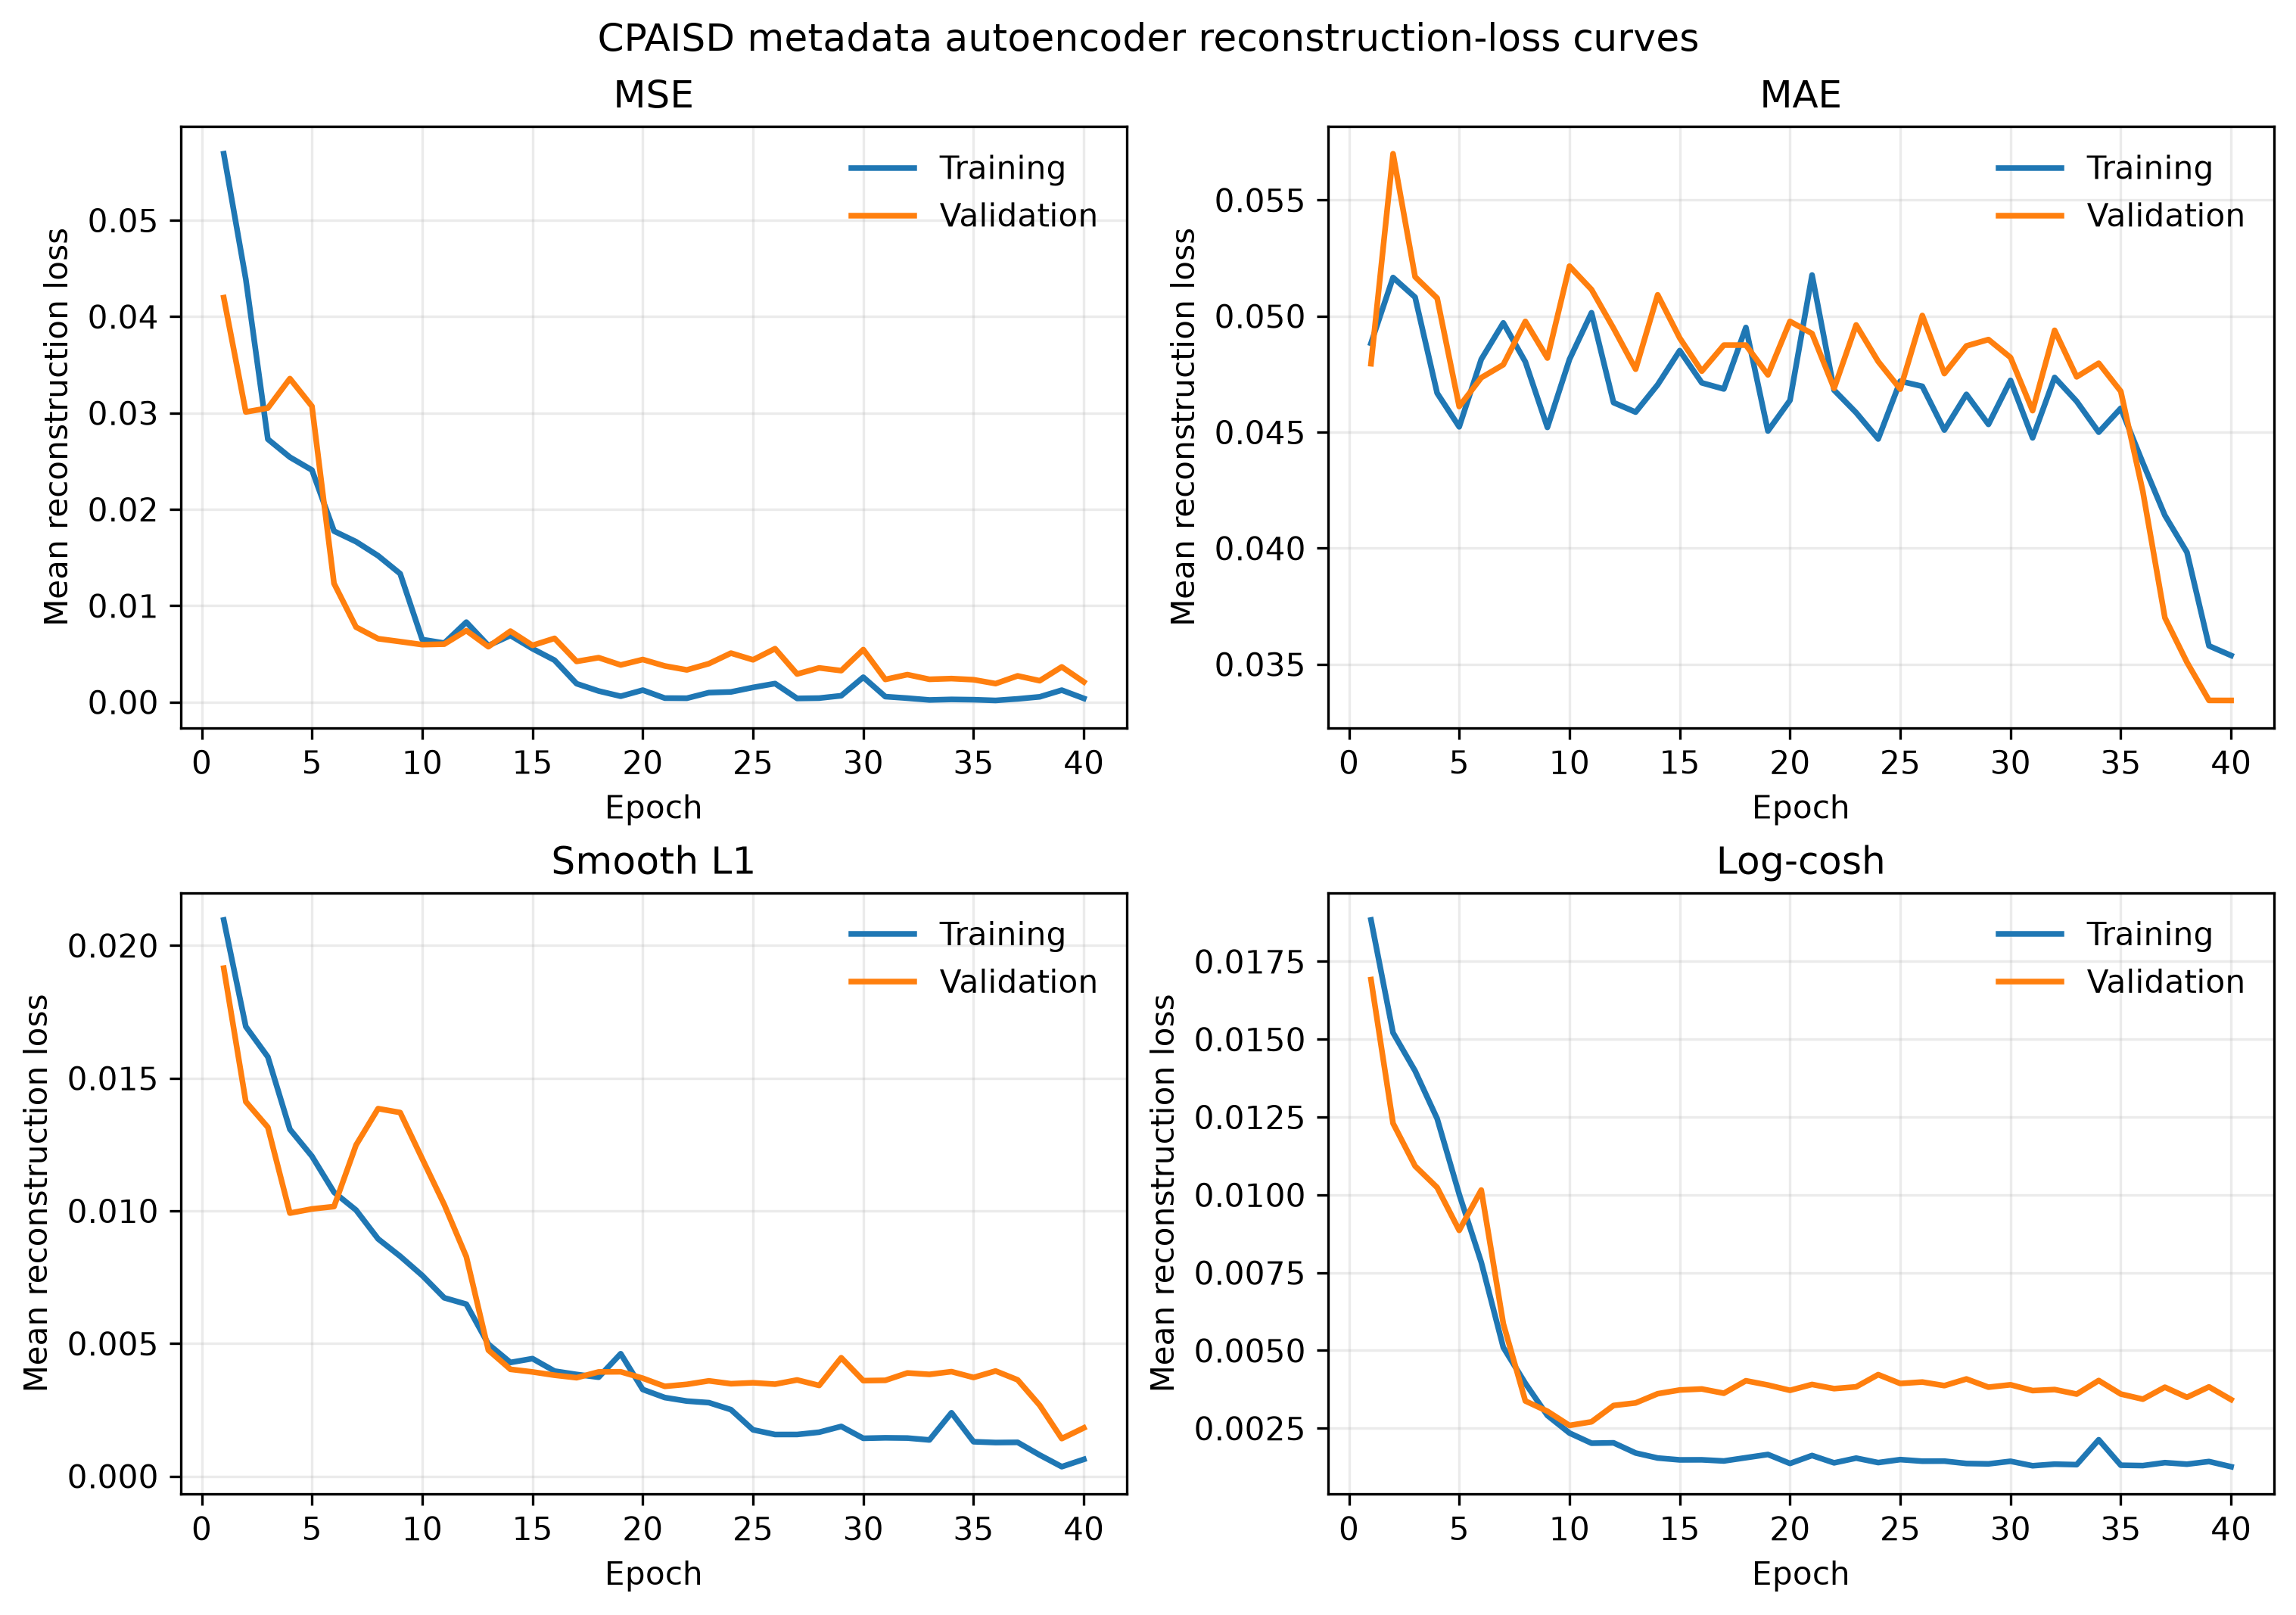
\includegraphics[width=0.96\textwidth]{autoencoder_loss_curves.png}
  \caption{Training and clean-validation objectives for the MSE, MAE, Smooth L1, and log-cosh autoencoders. Each panel uses its own vertical scale because the objectives have different numerical ranges.}
  \label{fig:ae_loss_curves}
  \end{figure*}

  \begin{figure*}[t]
  \centering
  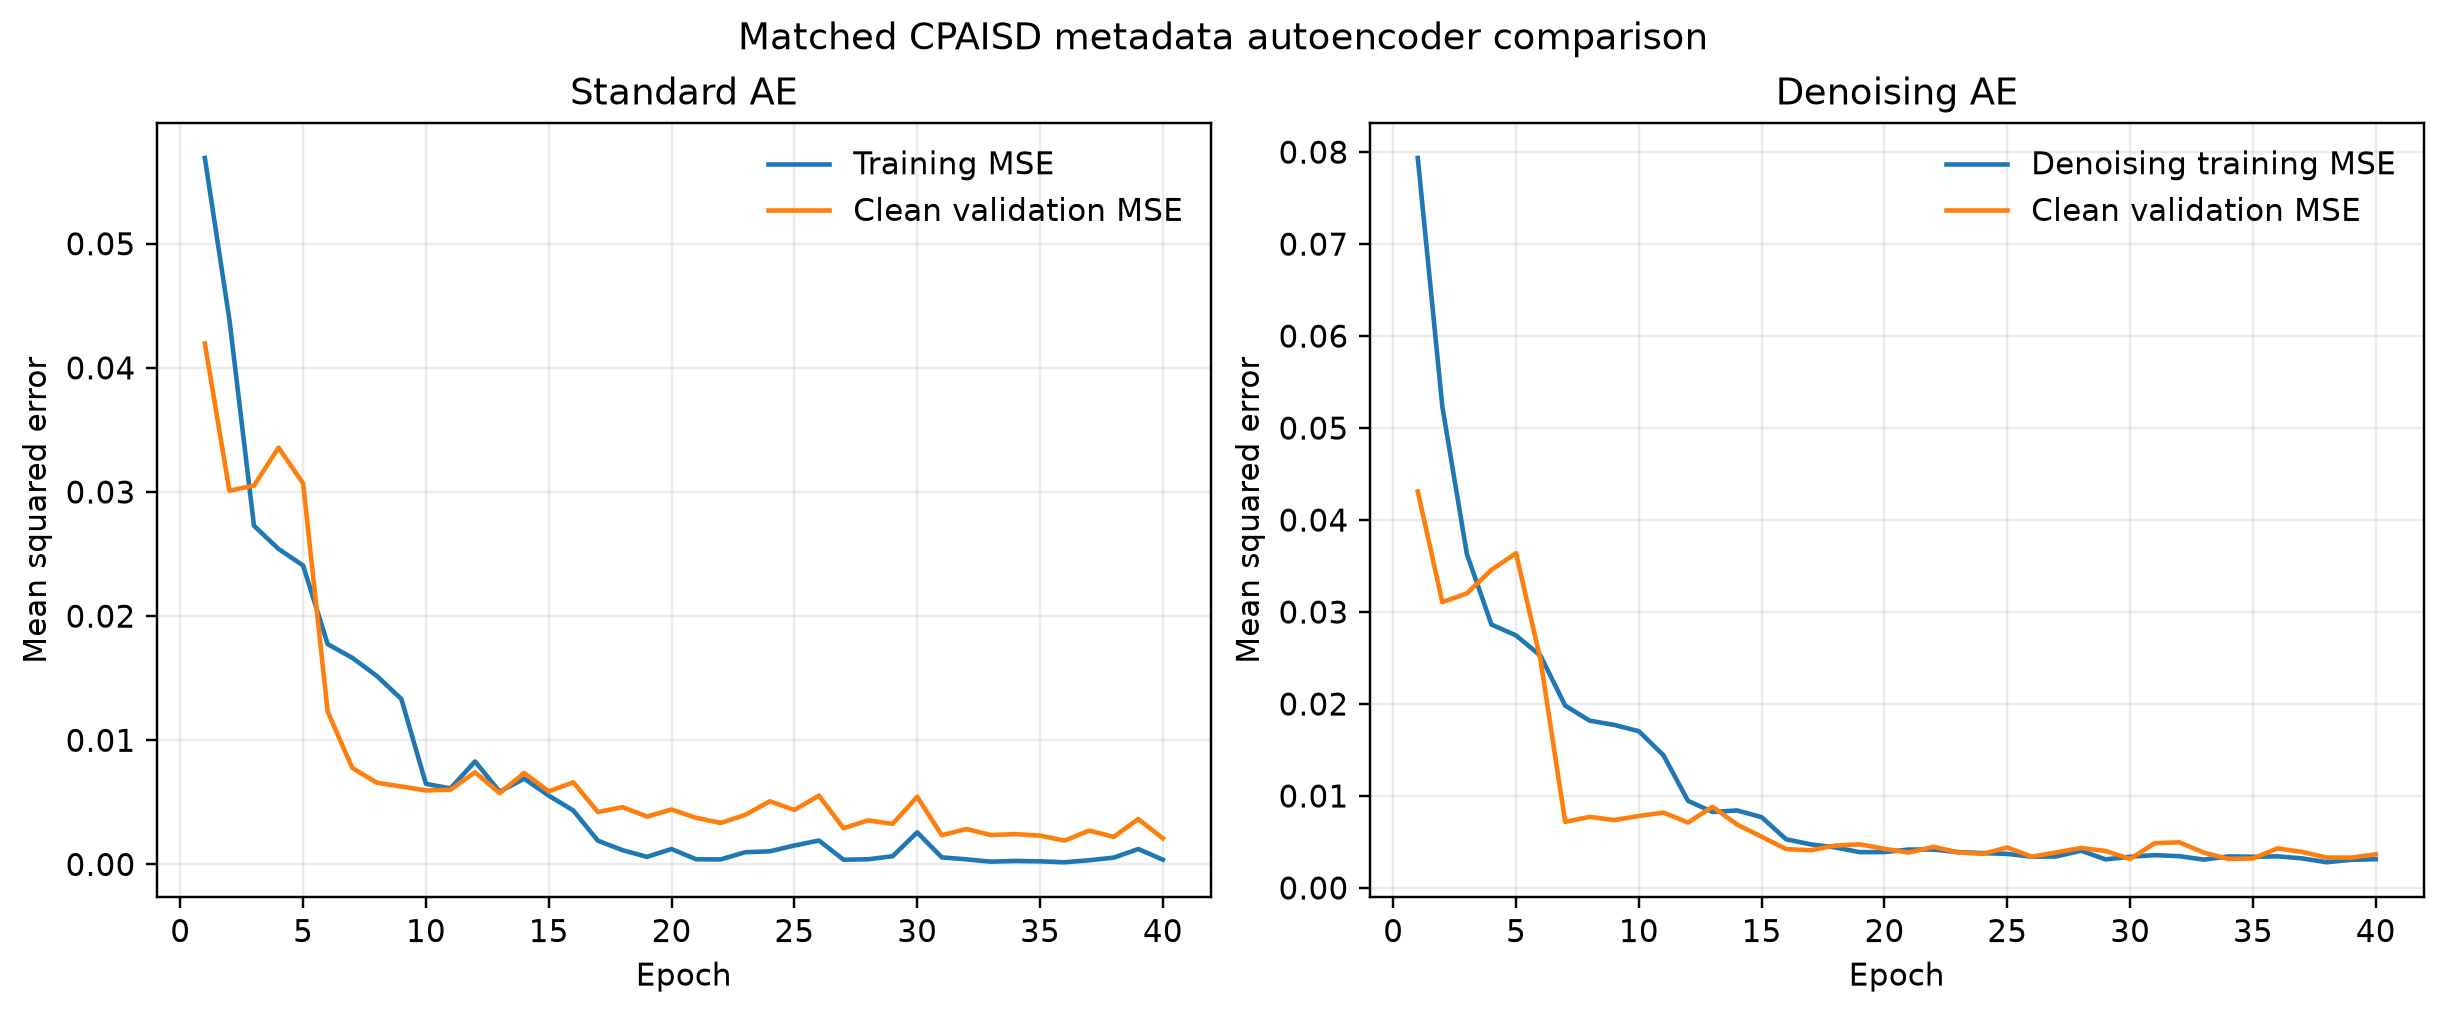
\includegraphics[width=0.88\textwidth]{denoising_autoencoder_curves.png}
  \caption{Training curves for the standard and denoising autoencoders. The denoising model receives noisy and partially masked training features but reconstructs clean feature targets.}
  \label{fig:denoising_ae_curves}
  \end{figure*}

  \begin{figure*}[t]
  \centering
  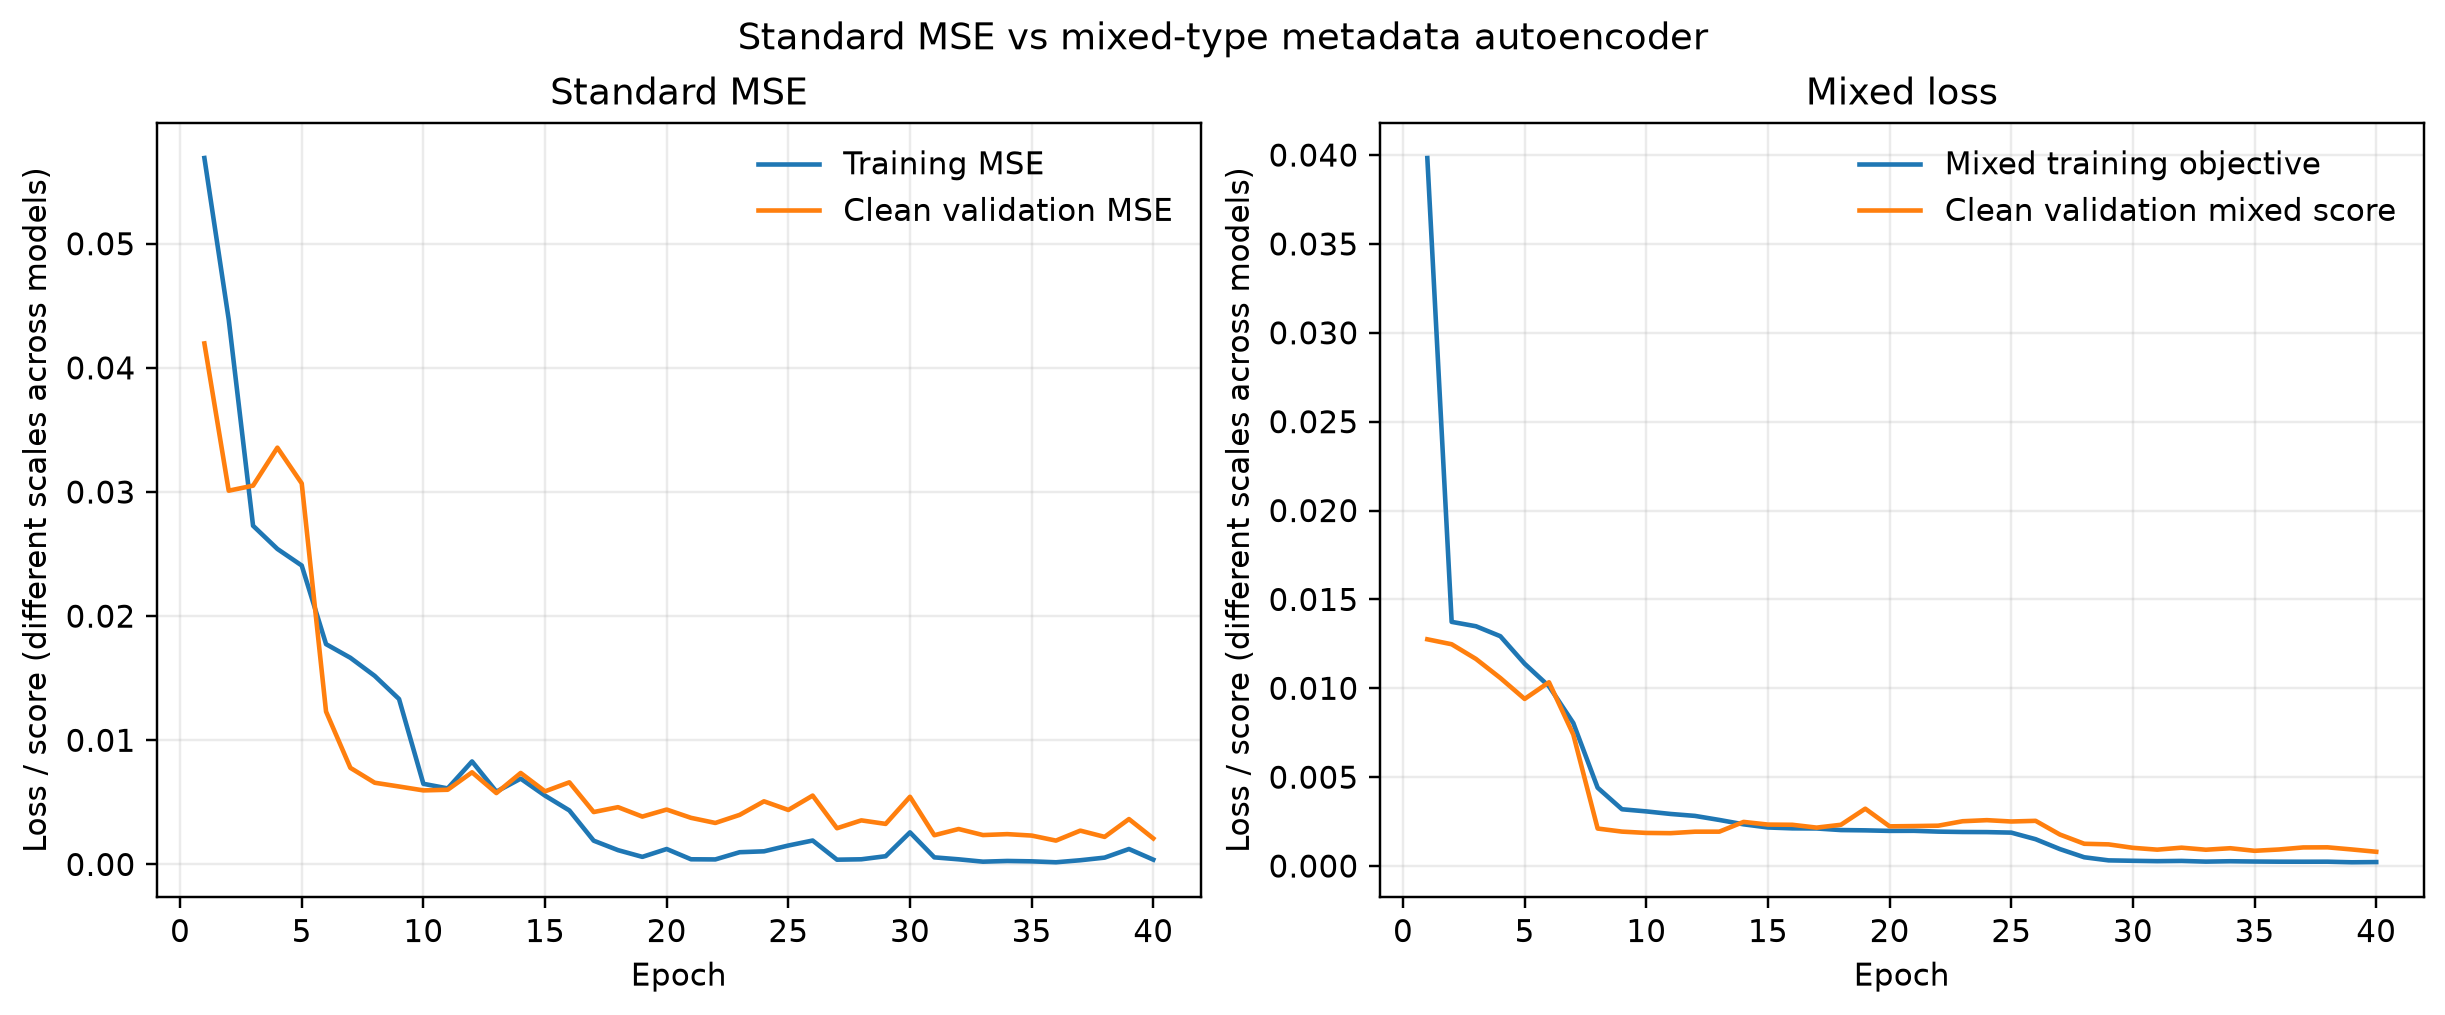
\includegraphics[width=0.88\textwidth]{fixed_mixed_autoencoder_curves.png}
  \caption{Training curves for the standard MSE and fixed equal-weight mixed-loss autoencoders. Curves describe optimization on this training run and do not by themselves measure tamper-detection quality.}
  \label{fig:fixed_mixed_ae_curves}
  \end{figure*}

  \begin{table*}[t]
  \caption{RMSprop metadata autoencoder reconstruction-objective comparison. Attack metrics are unweighted macro means over six scripted metadata conditions; clean FPR is measured on the 809-file test fold. Values are proportions.}
  \label{tab:ae_objectives}
  \centering\scriptsize
  \setlength{\tabcolsep}{5pt}
  \begin{tabular}{lrrrrrr}
  \toprule
  Objective & Attack macro F1 & Attack macro recall & Attack macro FPR & Clean file FPR & Clean study FPR & Seeds \\
  \midrule
  MSE & \textbf{0.831} & \textbf{0.833} & 0.002 & 0.0012 & 0.100 & 1 \\
  Denoising MSE & 0.667 & 0.667 & 0.000 & 0.0000 & 0.000 & 1 \\
  Fixed mixed (1/3 each) & 0.663 & 0.667 & 0.003 & 0.0025 & 0.100 & 1 \\
  Smooth L1 ($\beta=1$) & 0.603 & \textbf{0.833} & 0.206 & 0.1669 & 0.100 & 1 \\
  MAE & 0.600 & 0.572 & 0.000 & 0.0000 & 0.000 & 1 \\
  Log-cosh & 0.444 & 0.659 & 0.264 & 0.2138 & 0.200 & 1 \\
  \bottomrule
  \end{tabular}
  \end{table*}

  \subsection{Bilevel weighting of metadata reconstruction losses}
  In a matched single-seed comparison, Adam adapted the numerical, categorical, and presence-loss coefficients from equal initialization to 0.2065, 0.4299, and 0.3636. The bilevel model's file macro F1 was 0.562, a small increase over the matched MSE result (0.557), and its clean-test file FPR was 21.1\% versus 21.8\% for MSE. The fixed equal-weight mixed baseline had macro F1 0.463 and clean-test FPR 35.0\%. All three detectors had attack macro recall 0.833 under this split, and their clean study-level FPRs were 0.30, 0.30, and 0.40, respectively. Thus, the optimized weights improved file macro F1 slightly over MSE in this run, but the false-alarm rates remained high.

  \begin{table*}[t]
  \caption{Matched comparison of the MSE, fixed mixed, and Adam-bilevel mixed metadata autoencoders. Attack metrics are macro-averaged over six scripted conditions. Clean FPR is measured on the held-out test fold; values are proportions.}
  \label{tab:bilevel_metadata_loss}
  \centering\scriptsize
  \setlength{\tabcolsep}{5pt}
  \begin{tabular}{lrrrrrr}
  \toprule
  Model & Numeric / categorical / presence weights & Attack macro F1 & Attack macro recall & Attack macro FPR & Clean file FPR & Clean study FPR \\
  \midrule
  Standard MSE & -- & 0.557 & 0.833 & 0.268 & 0.218 & 0.300 \\
  Fixed mixed & 0.333 / 0.333 / 0.333 & 0.463 & 0.833 & 0.432 & 0.350 & 0.400 \\
  Bilevel mixed & 0.206 / 0.430 / 0.364 & 0.562 & 0.833 & 0.261 & 0.211 & 0.300 \\
  \bottomrule
  \end{tabular}
  \end{table*}

  Figure~\ref{fig:bilevel_metadata_weights} shows the evolution of the three loss-group coefficients. The coefficients are an optimization trajectory for one seed, not an uncertainty interval or evidence that the final mixture is optimal outside this protocol.
  \begin{figure*}[t]
  \centering
  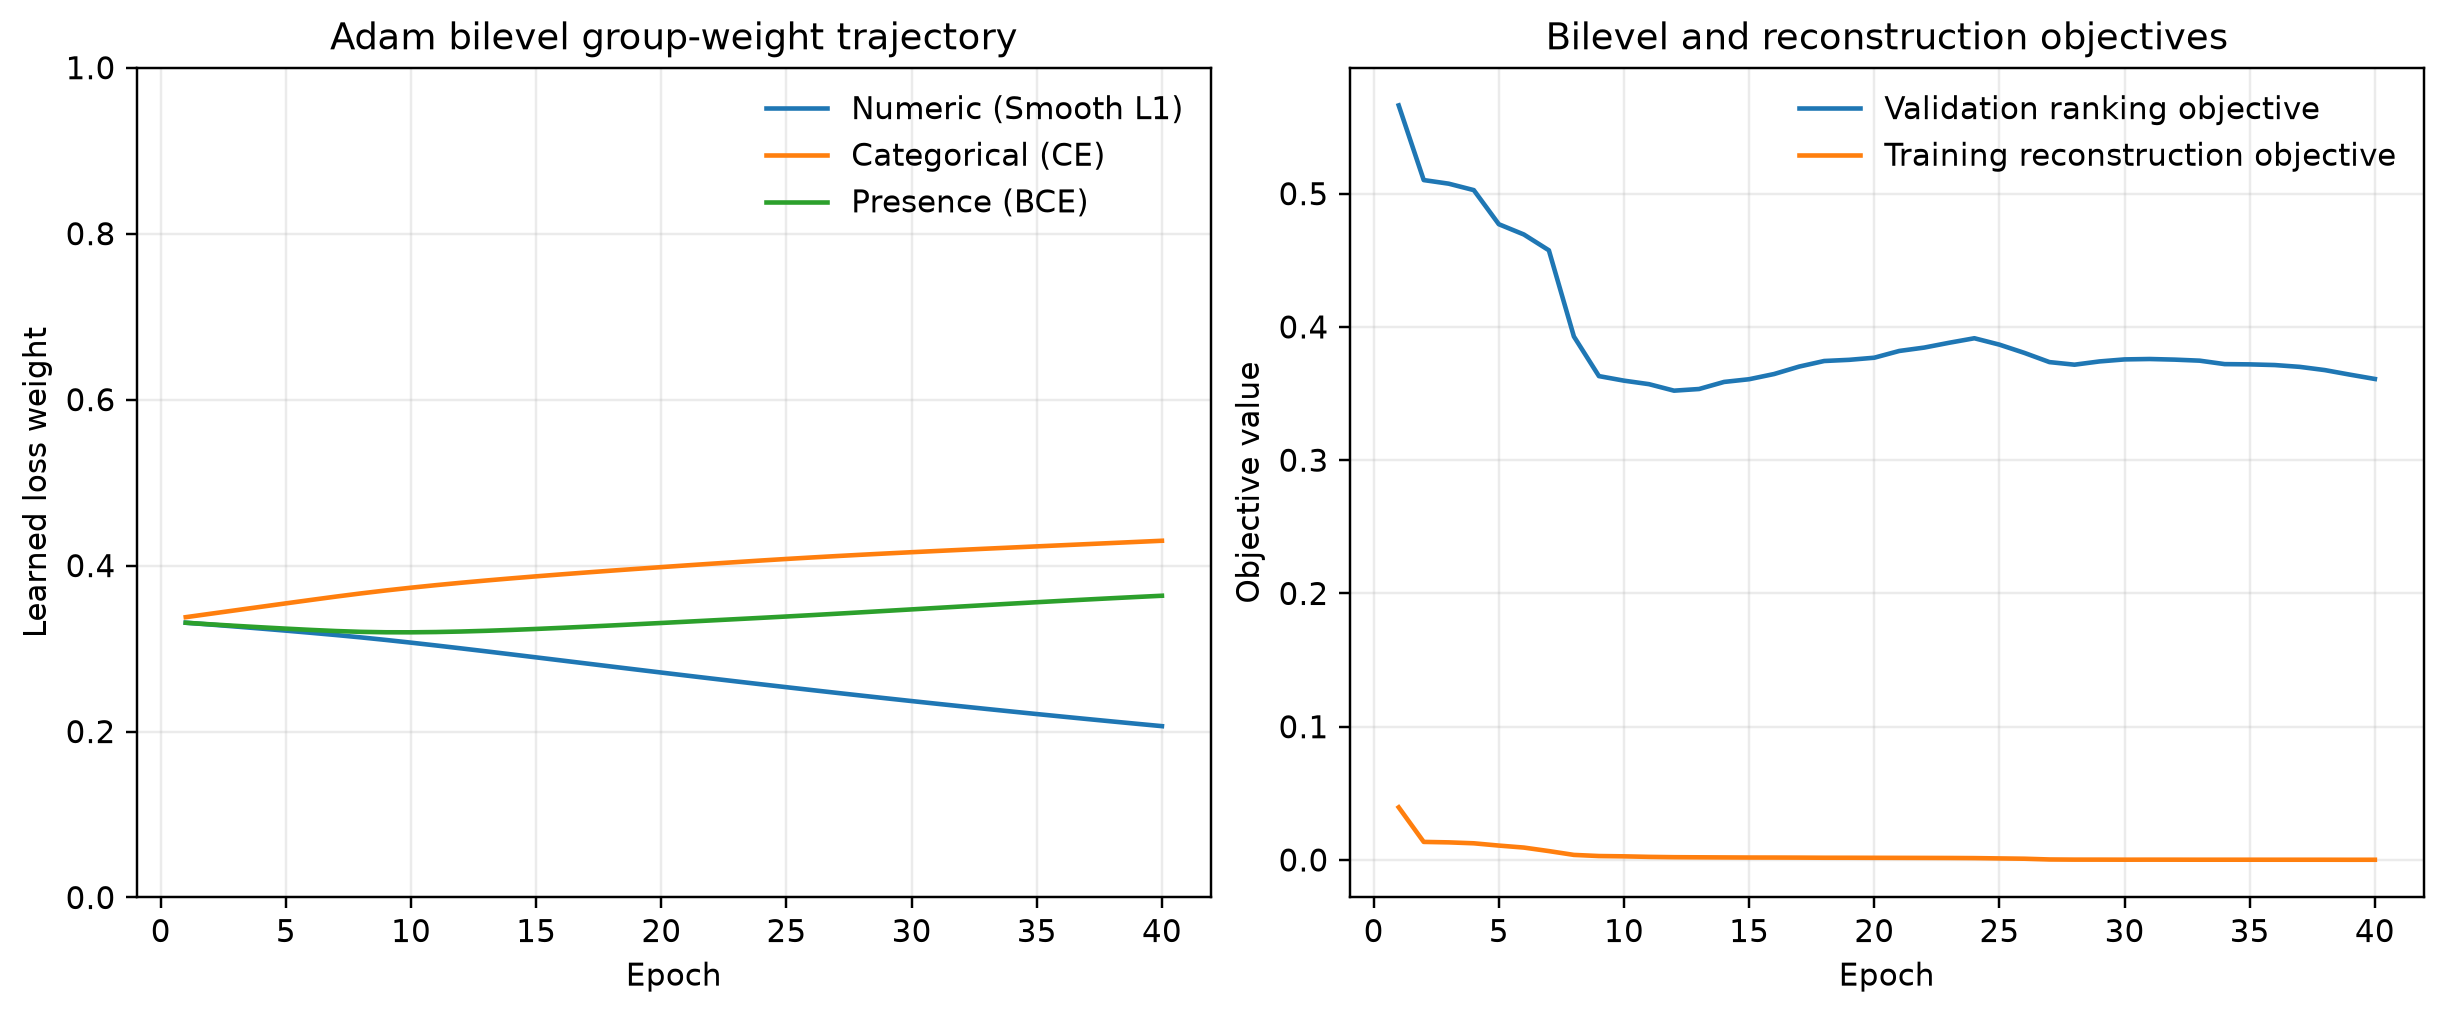
\includegraphics[width=0.96\textwidth]{bilevel_metadata_loss_weights.png}
  \caption{Adam-updated bilevel metadata reconstruction weights and training objectives over 40 epochs. RMSprop updates the autoencoder parameters; Adam updates the outer loss-group weights.}
  \label{fig:bilevel_metadata_weights}
  \end{figure*}

  \subsection{Three-seed fixed reconstruction-weight sweep}
  The 11-setting sweep evaluates fixed loss coefficients, rather than adapting them during training. None of the settings met the held-out validation clean-FPR target of 2\% in all three seeds. Every setting met it in exactly one seed; mean held-out validation FPR ranged from 14.8\% to 28.0\%. The equally weighted mixed loss had the lowest mean test clean FPR among the nine mixed settings (14.5\%) and a mean five-attack recall of 1.000. Since test metrics were reserved for descriptive reporting, this does not establish it as the selected or best setting. The marked variation across study splits shows that high recall on these synthetic attacks did not ensure cross-study false-alarm control.

  \begin{table*}[t]
  \caption{Three-seed reconstruction-loss weight sweep. Entries are mean $\pm$ standard deviation across seeds. Recall is macro-averaged over five whole-study metadata edits (UID inconsistency excluded); FPR is file-level. The final column counts seeds with held-out validation clean FPR $\leq2\%$. Test results are descriptive and were not used to select a setting.}
  \label{tab:ae_weight_sweep}
  \centering\scriptsize
  \setlength{\tabcolsep}{4pt}
  \begin{tabular}{lrrrrr}
  \toprule
  Setting & Validation recall & Validation clean FPR & Test recall & Test clean FPR & Target passes / 3 \\
  \midrule
  Plain MSE & 1.000 $\pm$ 0.000 & 0.280 $\pm$ 0.285 & 1.000 $\pm$ 0.000 & 0.171 $\pm$ 0.239 & 1 \\
  PixelSpacing-weighted MSE & 1.000 $\pm$ 0.000 & 0.168 $\pm$ 0.146 & 1.000 $\pm$ 0.000 & 0.204 $\pm$ 0.073 & 1 \\
  Mixed (0.20, 0.20, 0.60) & 0.976 $\pm$ 0.041 & 0.185 $\pm$ 0.160 & 0.933 $\pm$ 0.115 & 0.188 $\pm$ 0.183 & 1 \\
  Mixed (0.60, 0.20, 0.20) & 0.988 $\pm$ 0.022 & 0.148 $\pm$ 0.133 & 0.933 $\pm$ 0.115 & 0.164 $\pm$ 0.127 & 1 \\
  Mixed (0.20, 0.60, 0.20) & 1.000 $\pm$ 0.000 & 0.208 $\pm$ 0.187 & 1.000 $\pm$ 0.000 & 0.249 $\pm$ 0.264 & 1 \\
  Mixed (1/3 each) & 1.000 $\pm$ 0.000 & 0.163 $\pm$ 0.141 & 1.000 $\pm$ 0.000 & 0.145 $\pm$ 0.126 & 1 \\
  Mixed (0.50, 0.25, 0.25) & 1.000 $\pm$ 0.000 & 0.169 $\pm$ 0.146 & 1.000 $\pm$ 0.000 & 0.295 $\pm$ 0.092 & 1 \\
  Mixed (0.25, 0.50, 0.25) & 1.000 $\pm$ 0.000 & 0.170 $\pm$ 0.147 & 0.971 $\pm$ 0.050 & 0.218 $\pm$ 0.172 & 1 \\
  Mixed (0.25, 0.25, 0.50) & 1.000 $\pm$ 0.000 & 0.202 $\pm$ 0.191 & 1.000 $\pm$ 0.000 & 0.270 $\pm$ 0.267 & 1 \\
  Mixed (0.40, 0.20, 0.40) & 1.000 $\pm$ 0.000 & 0.181 $\pm$ 0.158 & 1.000 $\pm$ 0.000 & 0.204 $\pm$ 0.144 & 1 \\
  Mixed (0.20, 0.40, 0.40) & 0.999 $\pm$ 0.001 & 0.154 $\pm$ 0.134 & 1.000 $\pm$ 0.000 & 0.187 $\pm$ 0.182 & 1 \\
  \bottomrule
  \end{tabular}
  \end{table*}

  \subsection{Seed sensitivity and study-cluster uncertainty}
  Four representative metadata attacks were repeated with study-selection seeds 42, 43, and 44, keeping the same ten-study test fold, trained models, and validation thresholds. Each seed selected two studies; modified-file counts varied with the selected studies' slice counts. At study level, structural rules recalled both selected studies for modality and UID inconsistency in all three runs; Isolation Forest recalled both for PixelSpacing; and the autoencoder recalled both for the Manufacturer same-length edit. It did not detect the modality or UID edits. Table~\ref{tab:seed_sensitivity} reports the mean study-level autoencoder FPR and its stratified 95\% percentile bootstrap interval, resampling baseline-keyed studies within the positive and negative strata and averaging over seeds.
  
  \begin{table}[t]
  \caption{Study-level recall across three study-selection seeds and autoencoder study-level FPR with stratified 95\% study-bootstrap interval.}
  \label{tab:seed_sensitivity}
  \centering\scriptsize
  \begin{tabular}{lrrrr}
  \toprule
  Attack & Rules recall & IF recall & AE recall & AE FPR [95\% CI] \\
  \midrule
  Modality & 1.000 & 0.000 & 0.000 & 0.125 [0.000, 0.250] \\
  PixelSpacing & 0.000 & 1.000 & 1.000 & 0.125 [0.000, 0.250] \\
  Manufacturer substitution & 0.000 & 0.000 & 1.000 & 0.125 [0.000, 0.292] \\
  UID inconsistency & 1.000 & 0.000 & 0.000 & 0.125 [0.000, 0.250] \\
  \bottomrule
  \end{tabular}
  \end{table}
  
  The corresponding positive-unit recall intervals were degenerate at 0 or 1 because each detector made the same binary decision for both attacked studies across these three selections. This stability is conditional on one small test fold and deterministic attack scripts; the bootstrap does not create additional independent patients or support cross-site inference. The hash and OR hybrid are omitted from the table because their results follow directly from the per-file clean reference and inherit that construction.
  
  \subsection{Study-level conformal alert calibration}
  The clean validation fold contains ten studies, so its smallest attainable conformal $p$-value is 0.091. At nominal $\alpha=0.10$, the clean-test study FPR was 0.000 for Isolation Forest and 0.100 for the autoencoder. Across the three study-selection seeds, the calibrated Isolation Forest detected the two positive PixelSpacing studies in each seed (recall 1.000, FPR 0.000); the autoencoder detected the Manufacturer and PixelSpacing studies (recall 1.000 for each) but missed the Modality and UID events. The autoencoder's mean study FPR was 0.125 across attacked conditions. Table~\ref{tab:conformal_study} gives the mean across seeds. At $\alpha=0.05$, no studies could be flagged because this level is below the available $p$-value resolution. At $\alpha=0.20$, clean-test study FPR rose to 0.300 for Isolation Forest and 0.600 for the autoencoder. These results show the practical limit imposed by only ten validation studies; the nominal level does not ensure a population false-alarm guarantee.
  
  \begin{table}[t]
  \caption{Mean study-level recall/FPR at conformal $\alpha=0.10$ across three study-selection seeds.}
  \label{tab:conformal_study}
  \centering\scriptsize
  \begin{tabular}{lrr}
  \toprule
  Attack & Isolation Forest & Autoencoder \\
  \midrule
  Modality & 0.000/0.000 & 0.000/0.125 \\
  PixelSpacing & 1.000/0.000 & 1.000/0.125 \\
  Manufacturer substitution & 0.000/0.000 & 1.000/0.125 \\
  UID inconsistency & 0.000/0.000 & 0.000/0.125 \\
  \bottomrule
  \end{tabular}
  \end{table}
  
  \subsection{Benign-like changes versus scripted attacks}
  Three predeclared benign-like transformations were applied to copies of all 809 clean test instances: updating the file-meta ImplementationVersionName, performing a limited privacy-field cleanup proxy with de-identification markers, and reserializing through pydicom without a requested attribute edit. These transformations are experimental proxies, not outputs from a named PACS or a complete standards-conformant de-identification process. The audit found unchanged PixelData and unchanged non-target clinical attributes in all 809 files for each condition. The canonical metadata digest changed for all files in the first two conditions and for none in the reserialization condition.
  
  For each benign-like condition, alarm rate is the fraction of files flagged after transformation. The new-alarm rate counts only files that were not flagged in the corresponding untouched clean test file. This distinction matters for the autoencoder: it flagged 112/809 files (0.138) in each condition, but these were the same pre-existing clean-test alarms, so none were newly triggered by the transformation. The OR hybrid retained those 112 baseline alarms; it additionally flagged files when the strict metadata hash detected an actual covered metadata change. On the six existing scripted attack conditions, macro recall is the unweighted mean of file-level recall across attack types. All values are descriptive for these transformations and this test fold; the labels encode how the files were edited, not intent or clinical harm.
  
  \begin{table*}[t]
  \caption{Detector alarms on benign-like transformations and macro recall on six scripted metadata attacks. Benign cells show alarm rate/new-alarm rate relative to untouched files.}
  \label{tab:benign}
  \centering\scriptsize
  \setlength{\tabcolsep}{5pt}
  \begin{tabular}{lrrrr}
  \toprule
  Method & File-meta update & Privacy cleanup proxy & Re-serialization & Attack macro recall \\
  \midrule
  Metadata SHA-256 & 1.000/1.000 & 1.000/1.000 & 0.000/0.000 & 1.000 \\
  Structural rules & 0.000/0.000 & 0.000/0.000 & 0.000/0.000 & 0.333 \\
  Isolation Forest & 0.000/0.000 & 0.000/0.000 & 0.000/0.000 & 0.089 \\
  Autoencoder & 0.138/0.000 & 0.138/0.000 & 0.138/0.000 & 0.670 \\
  Metadata OR hybrid & 1.000/0.861 & 1.000/0.861 & 0.138/0.000 & 1.000 \\
  \bottomrule
  \end{tabular}
  \end{table*}
  
  \subsection{Pixel-integrity results}
  Table~\ref{tab:pixelresults} summarizes the independent pixel experiment. The reference PixelData hash flagged every edited file in all three conditions (177/177, 177/177, and 2/2) and produced no mismatches among untouched files. This perfect result is expected because the exact clean file is the reference. As a negative control, the metadata hash flagged none of the pixel-only edits. Its zero recall is expected because the edited files' metadata was unchanged; the resulting accuracy is dominated by the majority of unedited files and should not be read as useful pixel-attack performance.
  
  The low-amplitude condition changed approximately 1\% of stored pixel values with a mean absolute difference of approximately 0.010 stored-value units per edited image. The localized-patch and single-slice conditions changed approximately 0.0095\% of pixels on average, with mean absolute differences of 0.00305 and 0.000763, respectively. These values are computed in the stored integer domain and are not HU-based measures. They describe these scripted edits only.
  
  \begin{table*}[t]
  \caption{File-level results for the separate pixel-integrity experiment. Hash entries are recall/FPR; difference summaries are averaged over edited files.}
  \label{tab:pixelresults}
  \centering\footnotesize
  \begin{tabular}{lrrrrrr}
  \toprule
  Attack & $n_+$ & Pixel SHA-256 & Metadata SHA-256 & Changed-pixel fraction & MAE & Max. difference \\
  \midrule
  Localized patch & 177 & 1.00/0.00 & 0.00/0.00 & 0.00009537 & 0.003052 & 32 \\
  Low-amplitude perturbation & 177 & 1.00/0.00 & 0.00/0.00 & 0.00999832 & 0.009998 & 1 \\
  Slice inconsistency & 2 & 1.00/0.00 & 0.00/0.00 & 0.00009537 & 0.000763 & 8 \\
  \bottomrule
  \end{tabular}
  \end{table*}
  
  \subsection{No-reference pixel anomaly results}
  The clean-trained patch Isolation Forest used 50,000 patches sampled from 2,084 training files, with thresholds calibrated from 980 validation files. On 809 clean test files, the observed image-level false-positive rate was 0.0111 and the pixel-map false-positive fraction was 0.0191. The detector did not identify any attacked image at its calibrated image threshold across the three synthetic attack conditions. Its pixel-level localization was weak: for low-amplitude edits, precision was 0.0100, recall 0.0052, and IoU 0.0034; localized-patch and slice-inconsistency localization had zero recall. The second, $5\times5$ median-filter residual comparator had an 8.78\% clean-test image alarm rate and a 0.0125\% pixel-map alarm fraction. In attacked conditions, it detected 6.21\% of localized-patch images and 5.65\% of low-amplitude images, but also flagged 9.65\% of unmodified files in those conditions; it detected no slice-inconsistency images. Pixel-mask IoU was zero for localized and slice edits and 0.00012 for the low-amplitude edits. Thus neither no-reference baseline provided useful localization, and the residual comparator's modest image recall came with a high false-alarm rate. These findings show that the simple image-only baselines did not reliably detect the tested edits at their validation-calibrated operating points. The results are negative but informative: a no-reference detector is a harder problem than exact-reference hashing, and synthetic changed-pixel masks do not guarantee separability from normal CT texture.
  
  \subsection{Initial four-epoch U-Net pilot (superseded)}
  An initial compact U-Net pilot, following the encoder--decoder design used for biomedical segmentation \cite{ronneberger2015}, used 512 training-fold images and four CPU epochs (batch size 8, input resized to $256\times256$, base width 8). The training generator alternated between localized-patch and sparse low-amplitude edits and supplied their synthetic binary masks. The copy-move family was withheld from training. Pixel and image thresholds were calibrated from clean validation predictions at the 99.5th percentile of sampled pixel probabilities and the 99th percentile of image-maximum probabilities, respectively. This initial run used the final epoch and is retained below only as a baseline; the completed validation-selected 30-epoch evaluation follows. Table~\ref{tab:unet} reports image-level classification metrics across all 809 test images per condition and pixel-level pooled metrics over modified images only.
  
  The image AUROC was highest for sparse low-amplitude attacks (0.778), yet the thresholded image recall remained at or below 0.114 for every condition. Pixel IoU was 0.071 for localized patches, 0.222 for sparse perturbations, and 0.036 for the unseen copy-move condition. Clean-test image FPR was 0.0618 and the clean pixel alarm fraction was 0.0114. At study level, F1/FPR were 0.250/0.625 for localized patches and 0.500/0.500 for each of sparse and copy-move conditions. Therefore, this pilot provides a supervised no-reference localization comparison, but its thresholded detections and study-level false alarms are poor. The better ranking AUROC for sparse edits should not be mistaken for useful performance at the selected operating threshold.
  
  \begin{table*}[t]
  \caption{Four-epoch pilot U-Net performance. Image metrics use all 809 test instances per condition; pixel metrics pool pixels from edited instances only. The copy-move family was withheld from training.}
  \label{tab:unet}
  \centering\scriptsize
  \begin{tabular}{lrrrrrrr}
  \toprule
  Test edit & Image AUROC & Image AUPRC & Image recall & Image FPR & Image F1 & Pixel F1 & Pixel IoU \\
  \midrule
  Localized patch & 0.700 & 0.432 & 0.114 & 0.040 & 0.189 & 0.133 & 0.071 \\
  Sparse low-amplitude & 0.778 & 0.328 & 0.086 & 0.056 & 0.129 & 0.364 & 0.222 \\
  Copy-move (withheld family) & 0.718 & 0.256 & 0.065 & 0.061 & 0.095 & 0.070 & 0.036 \\
  \bottomrule
  \end{tabular}
  \end{table*}
  
  The initial pilot predicted masks and synthetic ground-truth masks were generated at the resized model grid. Figure~\ref{fig:unet} illustrates representative outputs from the completed 30-epoch model. In this initial pilot, sparse-edit pixel precision was 0.227 and study-level FPR was 0.500. These pilot metrics were superseded by the completed run below; both runs test only scripted attacks and do not establish generalization to naturally occurring tampering.
  
  \begin{figure*}[t]
  \centering
  \begin{minipage}[t]{0.32\textwidth}\centering
  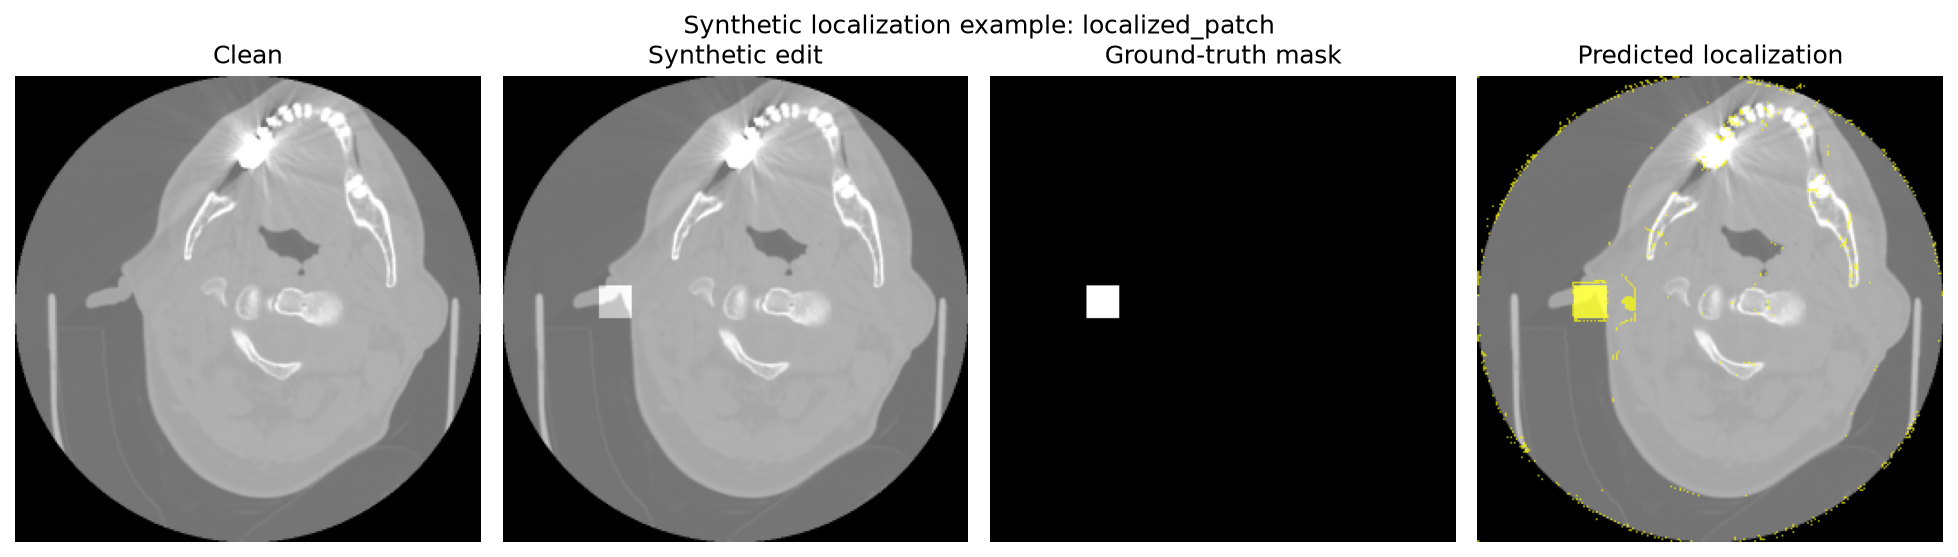
\includegraphics[width=\linewidth]{unet_localized_patch.png}\\[-2pt]
  \scriptsize (a) Localized patch
  \end{minipage}\hfill
  \begin{minipage}[t]{0.32\textwidth}\centering
  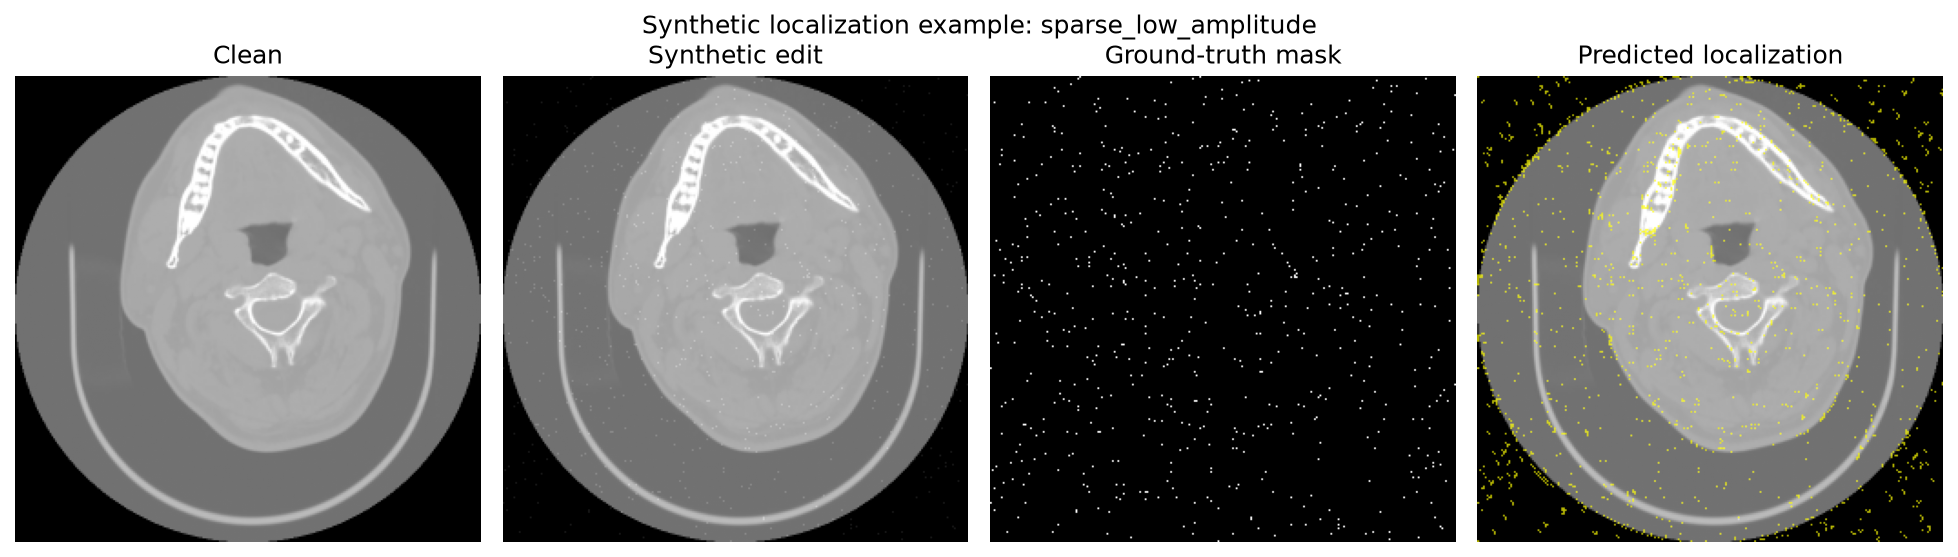
\includegraphics[width=\linewidth]{unet_sparse_low_amplitude.png}\\[-2pt]
  \scriptsize (b) Sparse low-amplitude edit
  \end{minipage}\hfill
  \begin{minipage}[t]{0.32\textwidth}\centering
  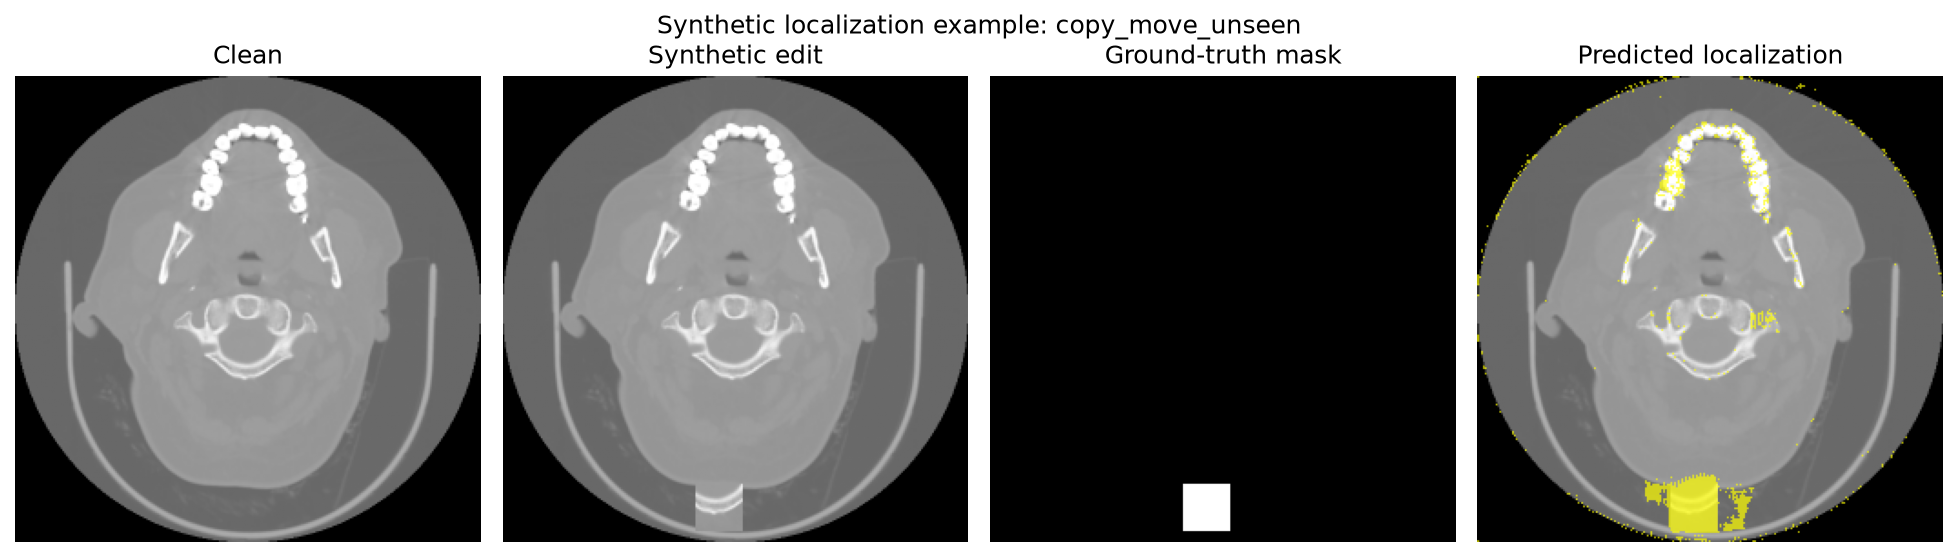
\includegraphics[width=\linewidth]{unet_copy_move_unseen.png}\\[-2pt]
  \scriptsize (c) Withheld copy-move edit
  \end{minipage}
  \caption{Representative inputs, synthetic ground-truth masks, and predictions from the completed 30-epoch U-Net. Outputs are displayed on the $256\times256$ model grid; these visual examples do not replace the quantitative test metrics.}
  \label{fig:unet}
  \end{figure*}
  
  \subsubsection{Completed validation-selected 30-epoch evaluation}
  The completed run used the same capped subset of 512 training images and finished all 30 epochs on CPU (about 49 minutes). Epoch 30 was selected by macro pixel IoU on the fixed synthetic-mask validation subset, with training loss 0.0603 and validation macro Dice/IoU of 0.9608/0.9254. Table~\ref{tab:unetval} reports family-wise validation metrics for 128 images per edit family. Because these measurements were used for checkpoint selection, they are not independent estimates. The selected model was then evaluated on all 809 held-out test images under three synthetic edit conditions, with each condition attacking two of the ten studies. Table~\ref{tab:unet30} reports the test results.
  
  Figure~\ref{fig:unet_training} shows the training loss and the synthetic-mask validation scores by epoch. Validation performance fluctuated, so the checkpoint was selected using the prespecified macro IoU criterion rather than the final training loss alone. The validation curves describe model selection on generated edits, not performance on naturally occurring tampering.
  
  \begin{figure*}[t]
  \centering
  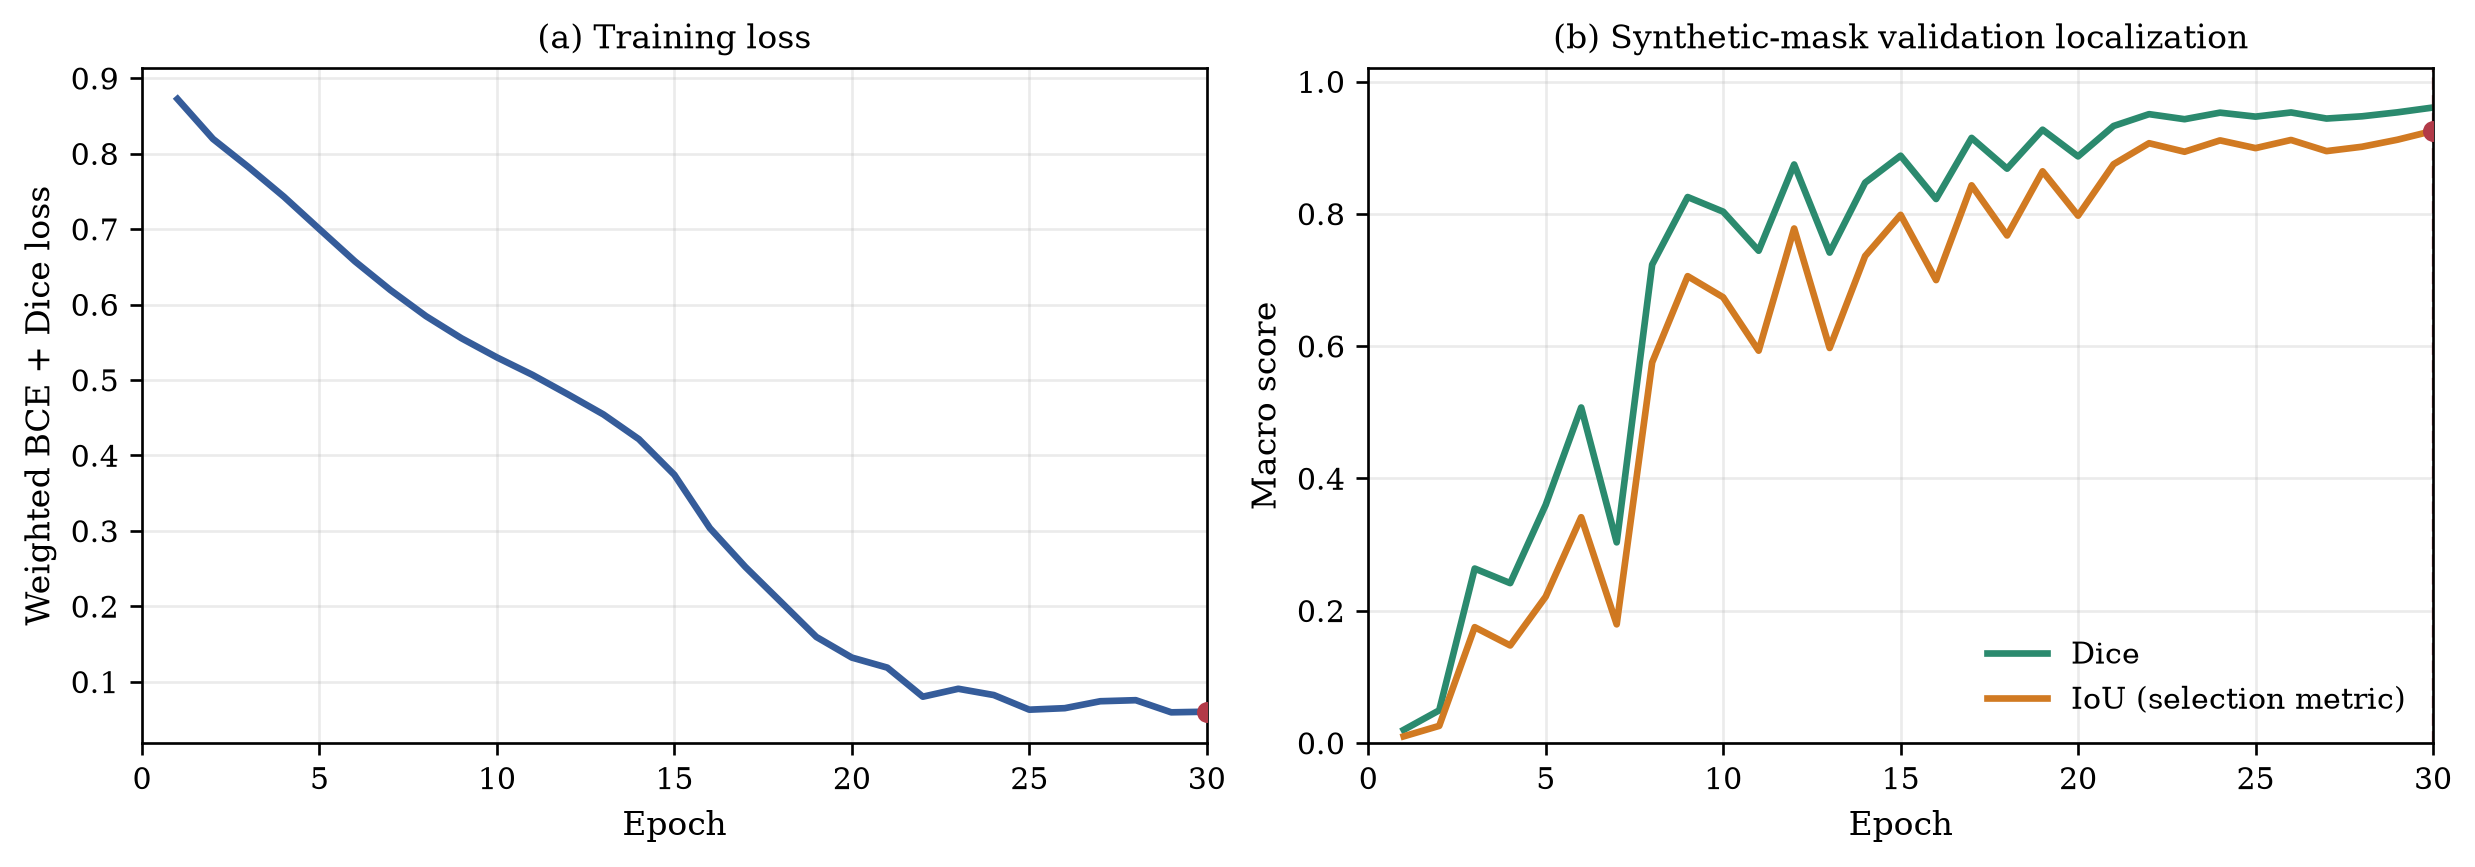
\includegraphics[width=0.96\textwidth]{unet_training_history.png}
  \caption{Training loss and validation localization scores for the 30-epoch U-Net. Validation scores are computed on 256 synthetic edited images (128 per training edit family) at a fixed probability threshold of 0.5; epoch 30 was selected by macro IoU. These validation data support checkpoint selection and are not independent test estimates.}
  \label{fig:unet_training}
  \end{figure*}
  
  \begin{table}[t]
  \caption{Synthetic-mask validation metrics for the selected epoch in the 30-epoch U-Net run. These are model-selection diagnostics, not independent test estimates.}
  \label{tab:unetval}
  \centering\scriptsize
  \begin{tabular}{lrrrr}
  \toprule
  Validation edit & $n$ & Pixel precision & Pixel recall & Dice / IoU \\
  \midrule
  Localized patch & 128 & 0.986 & 0.980 & 0.983 / 0.967 \\
  Sparse low-amplitude & 128 & 0.991 & 0.891 & 0.938 / 0.884 \\
  Macro mean & 256 & -- & -- & 0.961 / 0.925 \\
  \bottomrule
  \end{tabular}
  \end{table}
  
  \begin{table*}[t]
  \caption{Held-out test results for the validation-selected 30-epoch U-Net. Image metrics use all 809 test instances per condition; pixel metrics pool changed pixels over the attacked images. Copy-move was withheld from training.}
  \label{tab:unet30}
  \centering\scriptsize
  \setlength{\tabcolsep}{4pt}
  \begin{tabular}{lrrrrrrrrr}
  \toprule
  Edit family & $n_+$ & Image AUROC & Image AUPRC & Image recall & Image FPR & Image F1 & Pixel precision & Pixel recall & Pixel IoU \\
  \midrule
  Localized patch & 236 & 0.984 & 0.931 & 0.996 & 0.030 & 0.963 & 0.376 & 0.999 & 0.376 \\
  Sparse low-amplitude & 152 & 0.986 & 0.894 & 1.000 & 0.027 & 0.944 & 0.339 & 0.964 & 0.335 \\
  Copy-move (withheld) & 139 & 0.972 & 0.862 & 0.885 & 0.024 & 0.885 & 0.424 & 0.812 & 0.386 \\
  \bottomrule
  \end{tabular}
  \end{table*}
  
  On the untouched test fold, the observed image-level FPR was 0.0284 and the pixel alarm fraction was 0.0128. Although the file-level image F1 scores are high under these scripted conditions, pixel precision was 0.339--0.424, so many highlighted pixels were outside the synthetic masks. Study-level recall was 1.000 for all three conditions, but study-level FPR was 0.625 for localized patches and 0.500 for sparse and copy-move conditions. These point estimates come from only ten studies and two positive studies per condition; they do not establish reliable study-level detection or generalization. The pixel threshold selected from clean validation scores was 0.000858, and the image-score threshold was 1.000; this operating point and its calibration should be examined in follow-up work.

  \subsubsection{Attention U-Net architecture comparison}
  The Attention U-Net was trained with the same seed, 512-image training cap, 30-epoch budget, batch size, input resolution, synthetic edit families, and validation-selection procedure. It selected epoch 28 with validation macro pixel IoU 0.9322, compared with epoch 30 and 0.9254 for the standard U-Net. Table~\ref{tab:attention_compare} compares their held-out results. Attention increased pixel IoU for localized patches (0.376 to 0.397) and withheld copy-move edits (0.386 to 0.420), but reduced sparse-edit IoU (0.335 to 0.214). Image F1 was lower for all three families, and clean-test image FPR increased from 2.84\% to 3.83\%. Both models had identical study-level results: recall 1.000 and FPR 0.625 for patch edits, and recall 1.000 and FPR 0.500 for sparse and copy-move edits. Thus, the observed benefit is edit-family dependent and does not show overall superiority of the attention variant.

  \begin{table*}[t]
  \caption{Matched standard U-Net and Attention U-Net results. Pixel IoU and image F1 are evaluated on synthetic edits; clean image FPR is measured on the 809 untouched test instances.}
  \label{tab:attention_compare}
  \centering\scriptsize
  \begin{tabular}{lrrrrrrrr}
  \toprule
  Architecture & Best epoch & Val. IoU & Clean image FPR & Patch F1 / IoU & Sparse F1 / IoU & Copy-move F1 / IoU & Study FPR (patch/sparse/copy) \\
  \midrule
  Standard U-Net & 30 & 0.9254 & 0.0284 & 0.963 / 0.376 & 0.944 / 0.335 & 0.885 / 0.386 & 0.625 / 0.500 / 0.500 \\
  Attention U-Net & 28 & 0.9322 & 0.0383 & 0.957 / 0.397 & 0.924 / 0.214 & 0.836 / 0.420 & 0.625 / 0.500 / 0.500 \\
  \bottomrule
  \end{tabular}
  \end{table*}

  \subsubsection{Targeted adversarial evasion results}
  The FGSM/PGD evaluation reused the completed checkpoint and the same three synthetic test edit families, with two attacked studies per family. It evaluated only edited positive images; attack success is therefore conditional on baseline detection and does not estimate clean-image false-positive behavior under adversarial perturbation. Table~\ref{tab:fgsm_pgd} reports image recall, attack success rate (ASR), and pixel IoU. The fixed thresholds were taken from clean validation data; no test tuning was performed.

  \begin{table*}[t]
  \caption{U-Net evasion under bounded FGSM and PGD perturbations. Image recall is among synthetic edited positives. ASR is computed among images detected before attack; pixel IoU is against the original synthetic edit mask.}
  \label{tab:fgsm_pgd}
  \centering\scriptsize
  \begin{tabular}{lrrrrrrr}
  \toprule
  Edit family & Baseline recall & FGSM recall & FGSM ASR & FGSM IoU & PGD recall & PGD ASR & PGD IoU \\
  \midrule
  Localized patch & 0.996 & 0.877 & 0.119 & 0.032 & 0.097 & 0.902 & 0.081 \\
  Sparse low-amplitude & 1.000 & 0.217 & 0.783 & 0.019 & 0.000 & 1.000 & 0.117 \\
  Copy-move (withheld) & 0.885 & 0.547 & 0.390 & 0.026 & 0.173 & 0.805 & 0.057 \\
  \bottomrule
  \end{tabular}
  \end{table*}

  Under the tested budget, iterative PGD suppressed the image alarm on most baseline-detected examples: ASR ranged from 0.805 to 1.000. FGSM was less effective on localized patches (ASR 0.119) and more effective on sparse edits (0.783). After perturbation, pixel IoU fell substantially for all families. The PGD image recall of zero for sparse edits means none of the 152 edited images crossed the fixed alarm threshold, although residual pixel overlap remained (IoU 0.117). The results demonstrate sensitivity of this trained model to a targeted, white-box perturbation under the stated synthetic setup; they do not measure clinical plausibility, HU changes, or robustness of other detectors.
  
  \begin{table}[t]
  \caption{No-reference pixel detector performance. File FPR uses all 809 attacked-condition files; localization metrics aggregate only modified instances against their synthetic masks.}
  \label{tab:noref}
  \centering\scriptsize
  \begin{tabular}{lrrrr}
  \toprule
  Attack & IF recall/FPR & Residual recall/FPR & IF pixel IoU & Residual pixel IoU \\
  \midrule
  Localized patch & 0.000/0.014 & 0.062/0.097 & 0.00000 & 0.00000 \\
  Low-amplitude & 0.000/0.014 & 0.056/0.097 & 0.00343 & 0.00012 \\
  Slice inconsistency & 0.000/0.011 & 0.000/0.088 & 0.00000 & 0.00000 \\
  \bottomrule
  \end{tabular}
  \end{table}
  
  The clean-test file FPRs for the patch Isolation Forest and median residual comparator were 0.0111 and 0.0878, respectively. The latter's validation-calibrated 99th-percentile image threshold did not transfer to the clean test fold at the nominal tail rate. Its very small pixel-map FPR does not translate to useful localization because the synthetic edits are tiny relative to normal local image residuals. For each attack condition, unchanged copies have the same no-reference scores as their clean counterparts.
  
  \begin{figure*}[t]
  \centering
  \begin{minipage}[t]{0.32\textwidth}\centering
  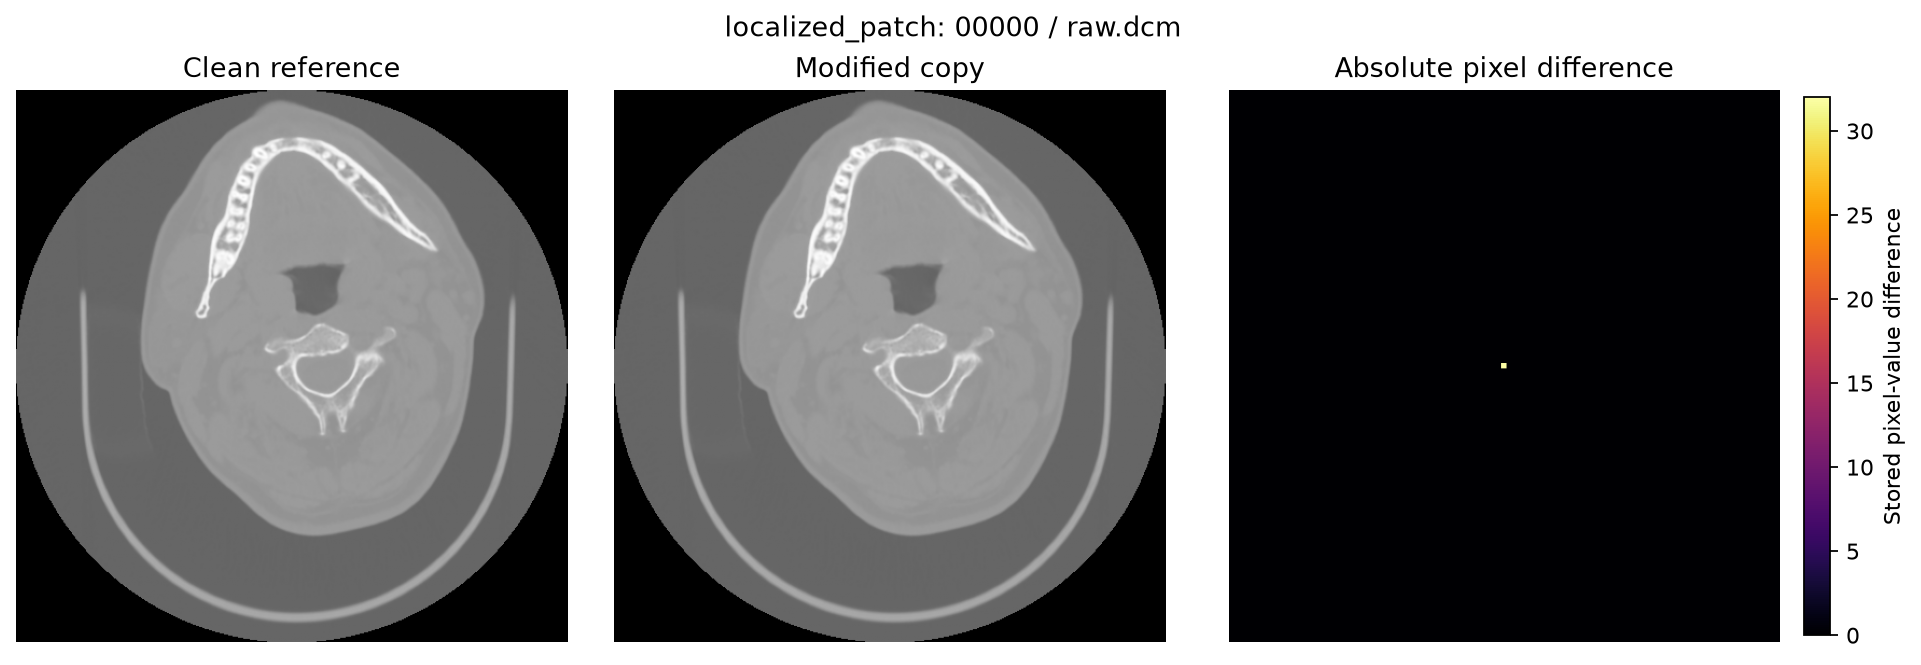
\includegraphics[width=\linewidth]{pixel_localized_patch.png}\\[-2pt]
  \scriptsize (a) Localized patch
  \end{minipage}\hfill
  \begin{minipage}[t]{0.32\textwidth}\centering
  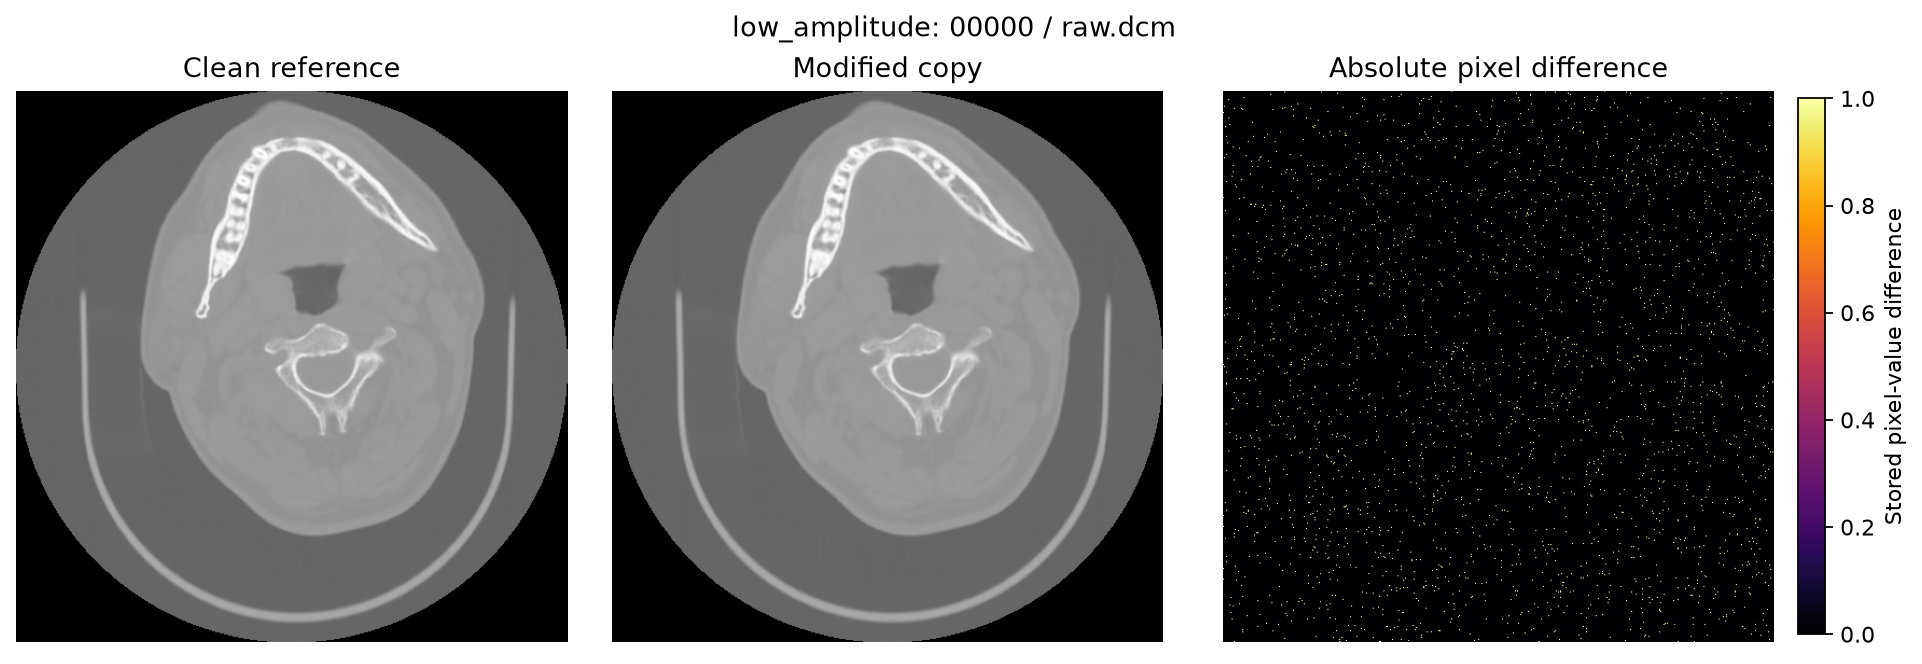
\includegraphics[width=\linewidth]{pixel_low_amplitude.png}\\[-2pt]
  \scriptsize (b) Low-amplitude perturbation
  \end{minipage}\hfill
  \begin{minipage}[t]{0.32\textwidth}\centering
  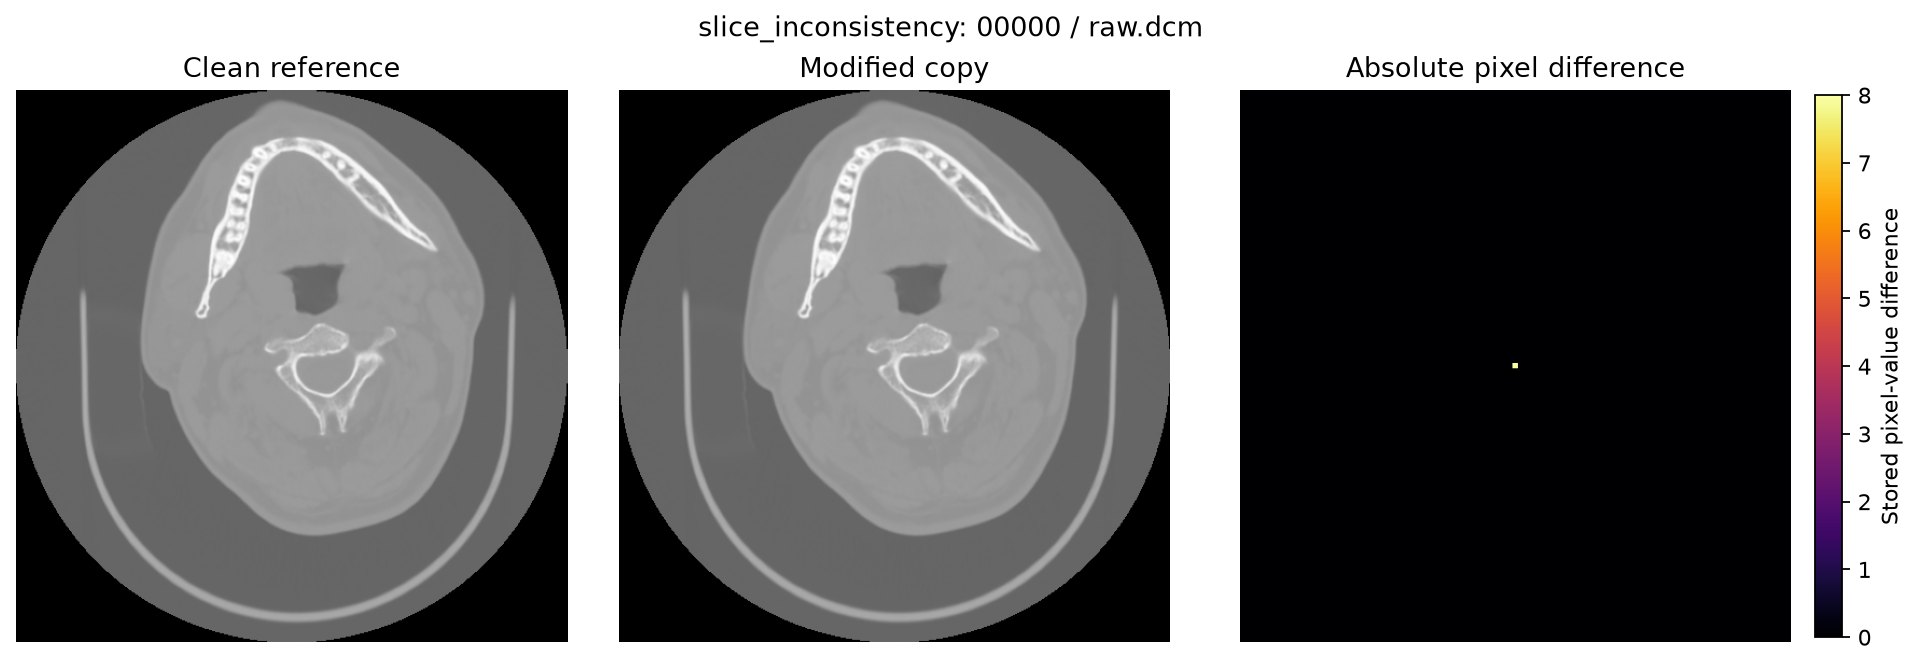
\includegraphics[width=\linewidth]{pixel_slice_inconsistency.png}\\[-2pt]
  \scriptsize (c) Slice inconsistency
  \end{minipage}
  \caption{Representative clean slice, modified copy, and absolute pixel-difference maps generated by the experiment. The difference scale is adjusted per example for visualization. These are reference-based visualizations, not outputs from an automated localization detector.}
  \label{fig:pixelheatmaps}
  \end{figure*}
  
  \subsection{Severity and mask-alignment results}
  Across all nine attack/severity combinations, PixelData SHA-256 achieved file-level recall 1.000 and FPR 0.000 against the per-file clean reference. The metadata hash achieved recall 0.000 on pixel-only conditions, as expected. Table~\ref{tab:severity} reports the perturbation magnitudes. The hash result does not vary with severity because any changed PixelData bytes produce a digest mismatch; this experiment does not establish the smallest perceptually or clinically meaningful change that could be detected.
  
  The reference-difference mask alignment yielded precision, recall, F1, and IoU of 1.000 for each of the three attack types. This is expected by construction: both the predicted region ($D_i>0$) and the target mask identify the pixels changed by the same script. These scores validate mask and difference-map bookkeeping; they must not be interpreted as localization performance on unknown tampering.
  
  \begin{table*}[t]
  \caption{Pixel attack severity summary. Changed-pixel fraction and MAE are averaged across modified files; the hash columns show file-level recall/FPR.}
  \label{tab:severity}
  \centering\scriptsize
  \begin{tabular}{llrrrr}
  \toprule
  Attack & Severity / parameters & $n_+$ & Changed-pixel fraction & MAE & Pixel SHA-256 recall/FPR \\
  \midrule
  Localized patch & Subtle: $3\times3$, $+1$ & 177 & 0.000034 & 0.000034 & 1.00/0.00 \\
  Localized patch & Default: $5\times5$, $+32$ & 177 & 0.000095 & 0.003052 & 1.00/0.00 \\
  Localized patch & Stronger: $9\times9$, $+32$ & 177 & 0.000309 & 0.009888 & 1.00/0.00 \\
  Sparse perturbation & Subtle: 0.1\%, $+1$ & 177 & 0.000999 & 0.000999 & 1.00/0.00 \\
  Sparse perturbation & Default: 1\%, $+1$ & 177 & 0.009998 & 0.009998 & 1.00/0.00 \\
  Sparse perturbation & Stronger: 5\%, $+2$ & 177 & 0.049999 & 0.099998 & 1.00/0.00 \\
  Slice inconsistency & Subtle: $3\times3$, $+1$ & 2 & 0.000034 & 0.000034 & 1.00/0.00 \\
  Slice inconsistency & Default: $5\times5$, $+8$ & 2 & 0.000095 & 0.000763 & 1.00/0.00 \\
  Slice inconsistency & Stronger: $9\times9$, $+32$ & 2 & 0.000309 & 0.009888 & 1.00/0.00 \\
  \bottomrule
  \end{tabular}
  \end{table*}
  
  \subsection{Combined metadata-plus-pixel results}
  The corrected combined run selected metadata- and pixel-attacked studies independently (seed 42 and seed 44, respectively). For each of four attack combinations, the metadata layer changed 177 files and the pixel layer changed 133 files in two other studies, yielding 310 unique positive files across four affected studies. Metadata-only and pixel-only SHA-256 checks detected 177/310 (0.571) and 133/310 (0.429) positives, respectively; their OR detected all 310 (recall 1.000), with zero observed false positives. This demonstrates complementary coverage of two exact-reference checks under independently sampled attacks. It does not show learned multimodal fusion or performance without trusted clean references.
  
  \begin{table*}[t]
  \caption{Combined metadata-plus-pixel attack results at file level. Entries are recall/FPR against the union attack labels.}
  \label{tab:combined}
  \centering\footnotesize
  \begin{tabular}{lrrrr}
  \toprule
  Condition & $n_+$ & Metadata SHA-256 & PixelData SHA-256 & OR of hashes \\
  \midrule
  PatientID insertion + localized patch & 310 & 0.571/0.000 & 0.429/0.000 & 1.000/0.000 \\
  PatientID insertion + low-amplitude & 310 & 0.571/0.000 & 0.429/0.000 & 1.000/0.000 \\
  Modality change + localized patch & 310 & 0.571/0.000 & 0.429/0.000 & 1.000/0.000 \\
  Modality change + low-amplitude & 310 & 0.571/0.000 & 0.429/0.000 & 1.000/0.000 \\
  \bottomrule
  \end{tabular}
  \end{table*}
  
  \subsection{Qualitative analysis}
  The attack outcomes illustrate the different operating principles. A modality change from CT to MR violates a fixed CT-only rule and is immediately detected. The original PatientID and StudyDescription scripts inserted tags that are absent in CPAISD, so their anomaly results may reflect a presence change rather than altered content. The same-length substitutions show field-dependent behavior: the autoencoder detected the Manufacturer edit but not the ProtocolName edit, despite preserved string length. This does not establish semantic detection of arbitrary plausible substitutions. PixelSpacing values remain finite and positive after multiplication by 1.7, so they pass the implemented range rule; learned-model response depends on the feature representation. For series UID inconsistency, the series-level rule flags all instances in an inconsistent series, while labels mark only the two modified files positive; neighboring slices are therefore counted as false positives at file level. Study-level grouping now uses the clean baseline UID, preventing UID edits from changing the aggregation key.
  
  The feature-aware ProtocolName attack explains the learned-detector blind spot: the same-length substitution leaves the current encoded input exactly unchanged, so all non-hash methods return the same prediction and scores as on the clean file. The header-to-pixel checker succeeds on the deliberately inconsistent dimension attacks because the declared layout conflicts with PixelData byte length and decoding. It does not flag value-only pixel edits that preserve the layout. Study-level conformal scores support a direct operating-point comparison but have only 10 calibration units; at $\alpha=0.20$, observed clean-test FPR rises sharply. Per-file explanation records list the alerting components, rule reasons, thresholds, and leading autoencoder reconstruction-error features. These are useful audit clues, but they do not establish causation or identify the exact changed tag for hash alerts.
  
  The new semantic consistency rules address a different case: a single slice contradicts values on its study or series peers. In the synthetic experiment, they detected both affected studies for four conditions that the existing structural rules missed: PatientID, ProtocolName, Manufacturer, and HighBit edits. They also detected both UID and modality positive controls, which the previous rules already flag. A follow-up coordinated ProtocolName edit showed the boundary directly: the checker recalled both studies when one instance changed, but recalled neither when all 177 instances in the same two studies were changed consistently. The reference hash detected both conditions. The study-level clean-control false-positive count was zero, but there were only ten studies; because findings propagate to peers, the checker marked 151--177 file records per single-instance condition. It cannot identify which member is the source of a group conflict, and a coordinated edit applied consistently across a whole group may pass.
  
  The per-attack F1 plot summarizes the metadata experiment only. Figure~\ref{fig:pixelheatmaps} shows representative pixel differences from the separate reference-based experiment; no image-content anomaly score is plotted.
  \begin{figure}[t]
  \centering
  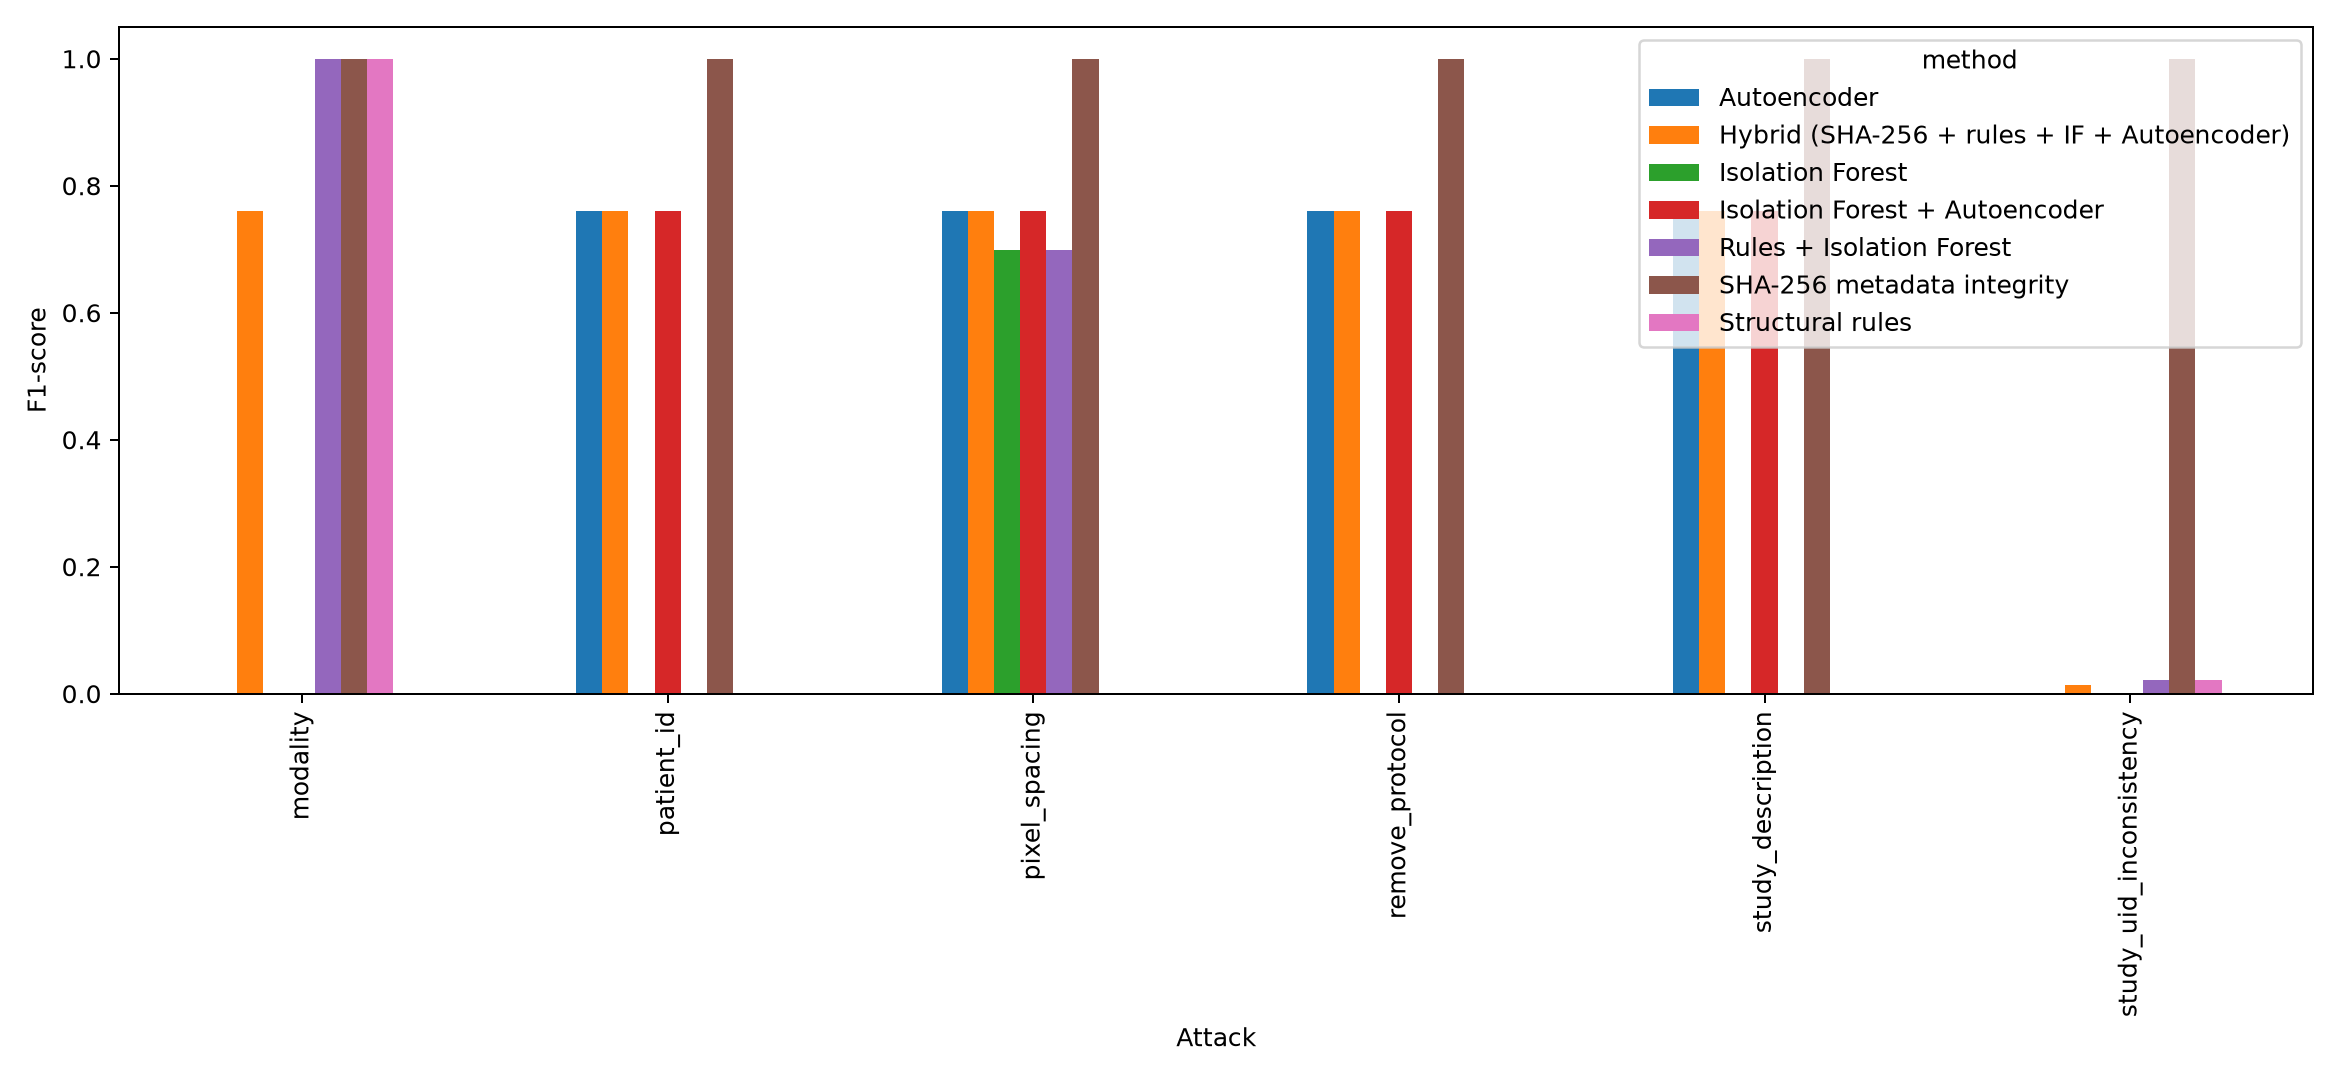
\includegraphics[width=\columnwidth]{f1_by_attack.png}
  \caption{Generated per-attack F1 plot. Hash-based performance is expected under the trusted-reference experiment.}
  \label{fig:f1}
  \end{figure}
  
  \begin{figure}[t]
  \centering
  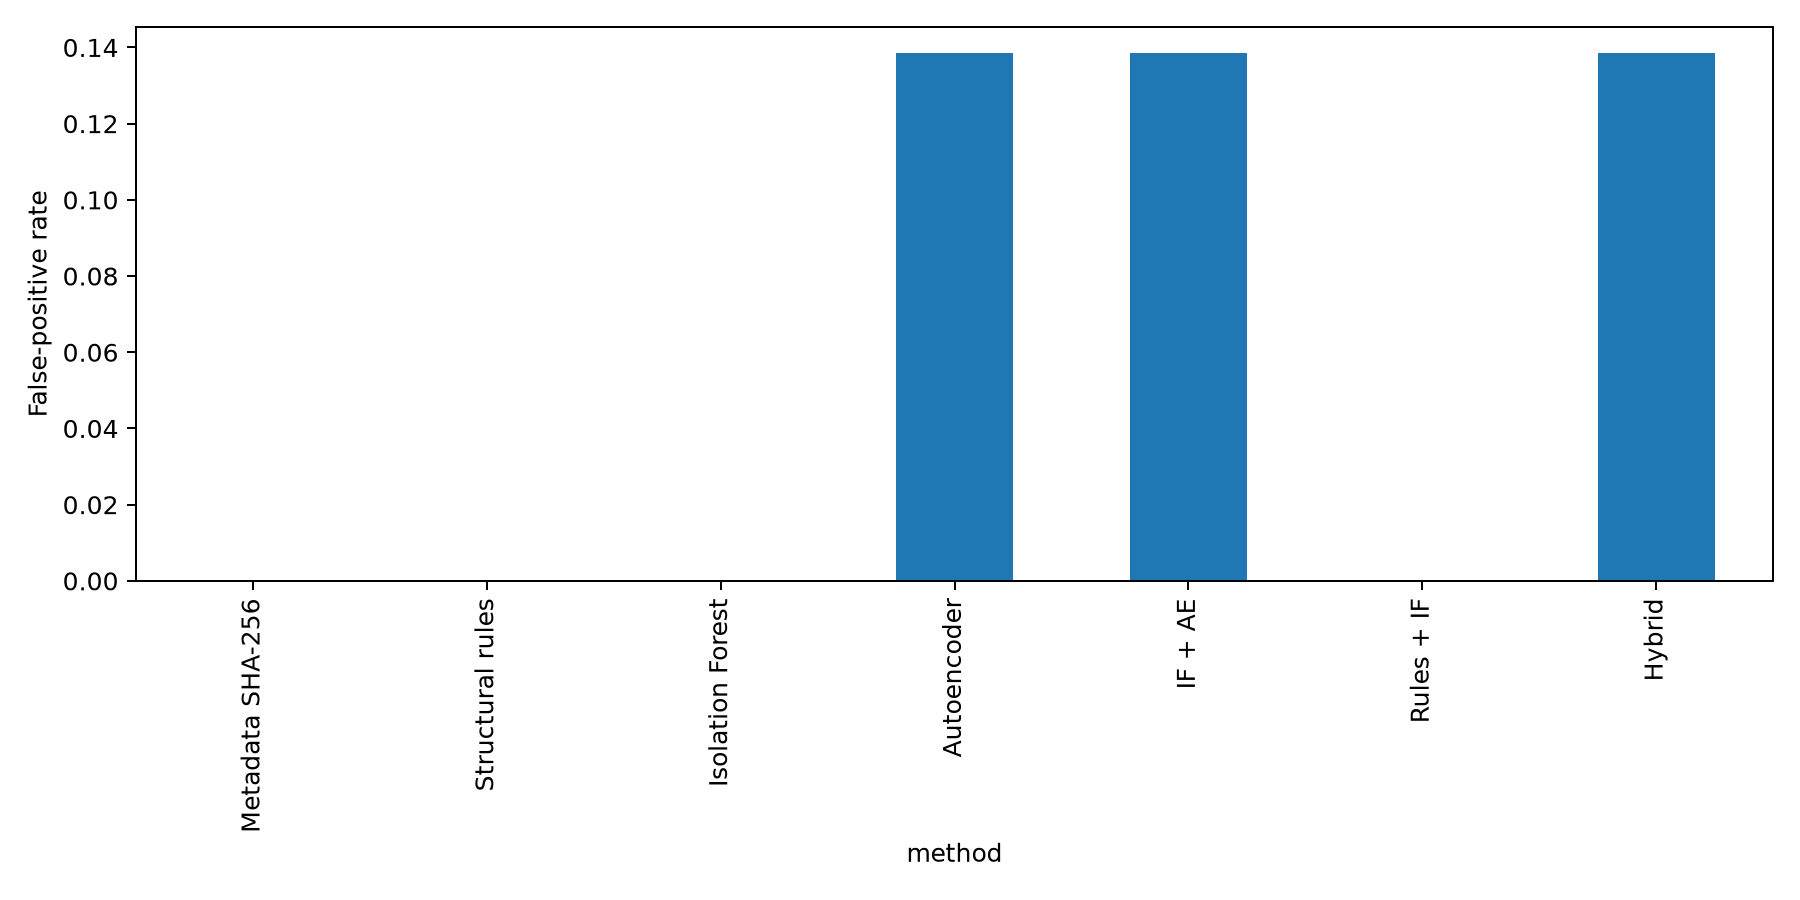
\includegraphics[width=0.9\columnwidth]{clean_test_fpr.png}
  \caption{Observed clean-test file false-positive rates. The test contains ten studies; these point estimates have high sampling uncertainty.}
  \label{fig:fpr}
  \end{figure}
  
  \subsection{Statistical interpretation}
  The original macro-average experiment did not compute inferential tests or confidence intervals. A later seed-sensitivity extension computed stratified study/series bootstrap intervals for four attacks, but these resample only ten studies from the same CPAISD test fold. Multiple slices within a study are correlated, and attack selections across seeds reuse the same ten studies. All results are descriptive for this attack-generation protocol; neither the bootstrap nor repeated seeds provide evidence of independent-site or population-level generalization.
  
  \section{Discussion}
  The experiments now include reference-based integrity checks, no-reference pixel baselines, header-to-pixel consistency rules, study/series metadata consistency, a feature-aware evasion condition, and study-level calibration. Pixel SHA-256 detected each modified file at every tested strength, as expected with a clean reference. The patch-level Isolation Forest failed to detect any of the three pixel attack types at its validation-calibrated image threshold. The median residual method detected only small fractions of two attack types at a 9.65\% condition-level FPR, with negligible mask localization. The header-to-pixel rules detected all deliberately inconsistent Rows/Columns conditions and no clean or pixel-only negative-control files. The new study/series checker detected both affected studies for four single-slice metadata conflicts missed by structural rules, with no false-positive study among eight unaffected studies per synthetic condition. This result is encouraging for internal consistency but remains based on ten studies and cannot catch coordinated values that remain consistent across a group. The ProtocolName feature-collision attack evaded every non-hash detector on 177/177 modified files, showing the cost of representing that field only by length and presence. At the study level, conformal calibration could distinguish some tested attacks at $\alpha=0.10$, but its resolution and false-alarm estimates are limited by ten validation studies. The per-file explanations expose detector sources and reconstruction-error features but are not causal explanations.

  The signed-manifest experiment adds sender authentication to the earlier reference-hash checks: a content digest alone can be recomputed by an attacker, while the receiver accepts a manifest only after verifying a signature from a locally trusted key. Across the 809-file test fold, all 13 scripted scenarios produced the expected status (Table~\ref{tab:signed_manifest_scenarios}). The preamble-only condition also separates byte-level from parsed-content integrity: a raw-file digest changed, while canonical metadata and PixelData remained equal and a content-only manifest verified. The outcomes support the prototype's intended checks, but do not estimate real transport performance or identify a hospital sender. Key issuance, private-key protection, trust-registry distribution and revocation, and replay state must be managed by a deployment. This is an application-layer file-transfer prototype; network throughput, DICOM association security, and interoperability were not evaluated.

  The separate U-Net robustness evaluation found that targeted PGD with a normalized-image $L_\infty$ budget of 0.02 reduced image recall to 0.000--0.173, with 0.805--1.000 attack success among images detected before attack. FGSM was weaker on localized patches and withheld copy-move edits, but still reduced sparse-edit recall to 0.217. Pixel IoU also fell substantially after both attacks. These results show that the learned localizer can be evaded by this white-box objective in the tested synthetic setting; they do not imply that small array-space perturbations are clinically plausible or survive conversion to DICOM/HU unchanged. An exact-reference hash would still detect a serialized PixelData change.
  
  The optimizer comparison favored RMSprop for this fixed configuration: it had the highest attack macro F1 at both file and study levels, and its clean-test file FPR was 0.12\%, compared with 13.84\% for Adam. All four optimizers flagged one of ten untouched studies; the clean study FPR therefore remained 0.10. This is a candidate result from one seed, not evidence that RMSprop is universally best. Repeated seeds and optimizer-specific learning-rate selection are needed before making a general claim.

  The reconstruction-objective experiments do not support a single loss as best under every criterion. In the full-fold, single-seed comparison, plain MSE had the highest attack macro F1 (0.831) and low clean file FPR (0.12\%); denoising MSE and MAE had zero observed clean alarms but lower attack F1. In the separate matched bilevel comparison, Adam learned numeric/categorical/presence weights of 0.206/0.430/0.364 and yielded macro F1 0.562 versus 0.557 for matched MSE, while both retained clean-test FPR above 21\%. This small difference is not persuasive evidence of improvement. The three-seed fixed-weight sweep likewise found no setting meeting its 2\% held-out validation FPR target consistently; its mean test clean FPRs remained high. These experiments use different calibration splits and protocols, so their absolute scores should not be ranked as one pooled benchmark. The loss curves document optimization behavior; detector quality must be judged from held-out detection metrics and false alarms.
  
  The hybrid's 100\% macro recall should not be read as a discovery that ML improves integrity protection. Since the hybrid is an OR over a SHA-256 reference check that has perfect recall by construction, its recall is inherited. Its FPR is higher than the hash-only FPR because an OR rule adds alarms from the autoencoder. Likewise, the pixel-hash result measures exact change against a trusted original; the heatmaps visualize differences using that same original and are not a no-reference detector. A more informative follow-up would compare non-hash detectors at a prespecified study-level FPR and evaluate a deployment-like setting where trusted reference availability is explicitly varied.
  
  The benign-change comparison further shows that a strict reference hash answers whether a covered value changed, not whether a change is malicious: it alarmed on the file-meta update and privacy-cleanup proxy, but not on metadata-preserving reserialization. The anomaly models did not add alarms beyond their existing clean-test flags for these conditions. The OR hybrid inherited hash alarms for the actual metadata edits. These results motivate testing documented exports from actual PACS systems before treating a hash mismatch as an operational security alarm.
  
  \section{Limitations}\label{sec:limitations}
  Several limitations constrain interpretation:
  \begin{enumerate}[leftmargin=*]
    \item \textbf{Small, single-center cohort.} CPAISD contains 112 studies from a narrow hyperacute stroke cohort; the test fold contains only ten studies. Cross-center generalization is untested.
    \item \textbf{Synthetic attacks and benign-like proxies.} Attack edits are deterministic scripted changes, not naturally occurring errors. In CPAISD, PatientID and StudyDescription were absent, so those conditions inserted tags rather than changing existing values. The feature-aware ProtocolName evasion is an explicit white-box feature collision, not a general adaptive attacker evaluation. The three benign-like transformations are controlled proxies; the privacy cleanup is limited, and none models a named PACS vendor or validated clinical workflow. The transformations do not establish whether a real change is harmless or malicious.
    \item \textbf{Reference leakage by design.} The metadata manifest is generated from the exact clean test objects later used as clean controls. This makes clean hash FPR zero by construction and supports only a controlled change-detection check. The manifest is not signed by this implementation.
    \item \textbf{Series/file label mismatch.} The UID attack changes one instance per selected series, but labels only the edited files as positive while the contextual rule flags neighboring slices. File-level false positives therefore include valid series-level detections. The corrected evaluation now reports metrics at the immutable baseline series unit, but the test contains only ten series, limiting precision of those estimates.
    \item \textbf{Feature limitations.} Several text fields are reduced to presence and length, and unknown categorical values can be discarded by the fitted vectorizer. The autoencoder may recognize the specific engineered length/value shifts without detecting semantically wrong but statistically ordinary substitutions.
    \item \textbf{Reconstruction-loss comparison scope.} The objective comparison uses one training seed and a single CPAISD split, while the bilevel metadata-weight comparison is also a single-seed run with a small observed macro-F1 difference from matched MSE and high clean false-alarm rates. The 11-setting fixed-weight sweep uses three seeds but only ten studies in each validation/test fold; no setting met the 2\% held-out validation FPR target across all seeds. These results are exploratory and do not establish an optimal loss or weights that generalize to other cohorts.
    \item \textbf{Optimizer-comparison scope.} Adam, RMSprop, AdamW, and SGD with momentum were each run once with seed 42, the same 40 epochs, and a shared learning rate. The comparison did not tune optimizer-specific learning rates or average over independent seeds. Its ranking is specific to this setup and ten-study test fold; RMSprop is the best observed setting here, not a general optimizer recommendation.
    \item \textbf{Semantic consistency scope.} The new rules compare selected fields assumed stable within a study or series and test six synthetic one-slice edits on only ten studies. Findings are propagated to group members, so they identify a conflicted group rather than the altered instance. Legitimate mixed-vendor or re-export variation may violate these assumptions, while a coordinated change that remains consistent across the group can evade the checker. Broader benign-control and multi-site evaluation is required.
    \item \textbf{Coordinated-edit scope.} The coordinated ProtocolName experiment changed every instance in two test studies and confirmed that internal-consistency checks alone miss a uniformly altered value. The experiment uses only two positive studies, one field, and one deterministic same-length substitution; it does not establish performance on other coordinated edits. Detection by the metadata hash depends on access to the exact clean reference.
    \item \textbf{Incomplete software provenance.} The run configuration records the seed and model parameters but not all package versions, hardware specifications, or deterministic-runtime settings. The reported elapsed time is not independently reproducible from the paper alone.
    \item \textbf{Limited pixel and adversarial evaluation.} The reference-difference/mask IoU is a bookkeeping check, and the no-reference patch Isolation Forest and median-filter residual baselines had poor detection or localization. The completed 30-epoch supervised U-Net was trained on a capped set of 512 images and achieved image F1 0.885--0.963 and pixel IoU 0.335--0.386 on three synthetic test conditions. However, pixel precision was only 0.339--0.424, and study-level FPR was 0.500--0.625 across only ten studies. Its validation masks and test attacks are synthetic, localization is measured on a resized $256\times256$ grid rather than native resolution, and edits are not calibrated in HU. The FGSM/PGD test is a targeted white-box attack against this one checkpoint, uses a fixed normalized-image budget and only positive synthetic edits, and does not assess clean-image adversarial false alarms or clinical plausibility. These array-space perturbations were not serialized back into DICOM for HU-domain assessment. BIM, C\&W, and DeepFool are not reported as completed experiments. The pixel editor supports uncompressed single-frame 2-D integer images.
    \item \textbf{Seed sensitivity scope.} The three-seed repeatability analysis changes which studies receive each synthetic attack but reuses the same ten-study test fold and fitted models. Its study-cluster bootstrap intervals do not account for site or population variation and may be degenerate when predictions are identical across seeds.
    \item \textbf{Coarse study calibration.} Conformal score calibration has only ten clean validation studies, so its minimum attainable $p$-value is $1/11$. The resulting operating points are coarse and do not guarantee a population-level false-alarm rate.
    \item \textbf{Simple cross-layer attacks.} Rows/Columns mismatch attacks create an obvious conflict between declared dimensions and payload length. The checker is not evaluated against plausible but incorrect metadata that still matches encoded layout, nor against every compressed or multiframe transfer syntax.
    \item \textbf{Explanation limits.} Autoencoder feature contributions summarize reconstruction error in the engineered representation. They are not causal attributions, and a reference hash alone cannot identify which metadata element changed.
    \item \textbf{Reference-based combined checks.} The independent combined run shows complementary coverage only because metadata and pixel SHA-256 digests are compared with exact clean references. It does not evaluate learned fusion, reference-free detection, or whether the clean manifest can be protected operationally. Benign-like controls show that strict digests alarm on covered metadata edits even when pixels and non-target clinical attributes are unchanged; testing with documented real PACS exports remains necessary.
    \item \textbf{Severity interpretation.} A cryptographic hash reports any changed byte, so perfect recall across the tested perturbation strengths is an expected property of the comparator. The sweep does not estimate perceptual detectability or a minimum clinically meaningful perturbation.
    \item \textbf{Signed-manifest and network scope.} The Ed25519 manifest is an external JSON sidecar, not a DICOM Digital Signature or a deployed PKI. Experiment keys were temporary, and the trust registry and replay cache were local demonstrations. The signed-manifest tests establish outcomes on this CPAISD fold but do not measure network throughput, latency, packet loss, concurrent load, DICOM association behavior, key lifecycle, or interoperability. HMAC is shared-key authentication and cannot identify which key holder generated a tag. The limited research-copy de-identification does not implement the complete DICOM PS3.15 confidentiality profile or assess pixel cleaning \cite{dicomps315}.
    \item \textbf{No clinical or forensic validation.} The metadata, pixel, and signed-manifest experiments do not establish clinical correctness, operational sender attribution, audit provenance, resistance to compromised endpoints or baselines, or malicious intent.
  \end{enumerate}
  
  \section{Conclusion and Future Work}
  This paper reports exploratory metadata, study/series consistency, coordinated metadata edits, reference-based pixel-integrity, no-reference pixel anomaly, cross-layer consistency, study calibration, benign-change control, adaptive-evasion, FGSM/PGD robustness, severity-sweep, combined-edit, autoencoder optimizer-comparison, and supervised-localization experiments on official CPAISD folds. In the original metadata experiment, macro F1 was 1.000 for metadata SHA-256, 0.170 for structural rules, 0.116 for Isolation Forest, and 0.506 for the autoencoder; the OR hybrid achieved 0.635 macro F1 with 0.207 macro FPR. In a separate six-objective comparison, MSE had the strongest macro F1 (0.831) among the tested single-seed reconstruction objectives. Adam-bilevel weighting of numeric, categorical, and presence losses reached weights 0.206/0.430/0.364 and macro F1 0.562 versus 0.557 for matched MSE, but both had clean-file FPR above 21%; the three-seed fixed-weight sweep found no setting meeting the 2% validation FPR target in all seeds. These protocols are distinct and do not establish a universally best loss. In a matched 40-epoch optimizer comparison, RMSprop had the highest autoencoder attack macro F1 (0.831 file-level; 0.667 study-level) and the lowest clean-test file FPR (0.0012); its clean study FPR was 0.100, or one of ten studies. This single-seed comparison used a shared, untuned learning rate. A feature-aware same-length ProtocolName edit preserved the model input in all 177 modified files and evaded each non-hash detector, while the reference hash detected all changes. The semantic checker detected 2/2 affected studies and had 0/8 false-positive studies for each of four synthetic one-slice conflicts missed by structural rules; UID and modality positive controls were detected by both. In a separate coordinated-edit condition, it detected 2/2 studies after one instance was changed, but 0/2 when ProtocolName was changed consistently across all instances in the two selected studies; the metadata reference hash detected both conditions. These results illustrate the limits of internal consistency checking and are based on only ten test studies. Cross-layer layout rules detected all 177 Rows and Columns mismatches and had no findings on clean or pixel-only control files. At study-level conformal $\alpha=0.10$, the clean-test FPR was 0 for Isolation Forest and 0.10 for the autoencoder, with only ten validation studies available for calibration. The no-reference patch Isolation Forest did not detect the scripted pixel attacks at its calibrated image threshold; a median-residual comparator detected 5.6--6.2\% of two image-level conditions with 9.65\% condition-level FPR and negligible localization. The completed 30-epoch U-Net, trained on 512 images with a validation-selected checkpoint, achieved image F1 0.885--0.963 and pixel IoU 0.335--0.386 across three synthetic test conditions. Its clean-test image FPR was 2.84\%, but pixel precision remained 0.339--0.424 and study-level FPR was 0.500--0.625 across ten studies. In the separate targeted evasion test ($L_\infty=0.02$), PGD achieved ASR 0.805--1.000 and reduced image recall to 0.000--0.173; FGSM achieved ASR 0.119--0.783. Pixel IoU fell under both attacks. These results show susceptibility of this checkpoint to the specified synthetic white-box attacks, not general attack success in clinical workflows. Pixel SHA-256 detected all edits across tested severities against the exact clean reference. Three benign-like controls preserved PixelData and non-target clinical attributes in all 809 files: the strict metadata hash alarmed on all file-meta and privacy-marker edits but not on metadata-preserving reserialization. The autoencoder's 112 clean-test alarms persisted unchanged across all three conditions. These findings remain descriptive for one ten-study test fold and do not show generalization to another dataset, robust adaptive resistance, or clinical utility.
  
  The signed-manifest extension demonstrates a reproducible sender--receiver integrity check in a local experiment: all 13 scripted security scenarios returned the expected status on 809 CPAISD test objects. Signing and verification averaged 15.44 and 12.82 ms per file, respectively, with a mean sidecar size of 868 bytes. The unsigned-reference control shows why an unauthenticated digest cannot establish provenance. These outcomes support inclusion of authentication as a complementary integrity layer; they are not evidence of a deployed secure DICOM network, DICOM Digital Signature conformance, or measured network performance.

  Before publication or stronger claims, the semantic rules need evaluation on more independent studies and benign metadata variation to test their assumptions about within-series consistency. The matched Attention U-Net comparison showed mixed effects: a small gain in patch and copy-move pixel IoU, a substantial drop for sparse-edit IoU, lower image F1 across families, and a higher clean image FPR. Repeated seeds and an attack evaluation of the attention checkpoint are needed before drawing broader conclusions about its usefulness or robustness. The completed 30-epoch and FGSM/PGD runs provide held-out results only for one ten-study cohort and scripted edits; study-level false alarms and the demonstrated PGD susceptibility limit practical interpretation. The adversarial experiment should be extended to multiple budgets, random starts, attack objectives, and independent cohorts, with careful assessment of whether perturbations remain clinically plausible after conversion to stored pixel values and HU. The no-reference pixel models also need improved features and more realistic pixel changes. The header-to-pixel rules should be tested on plausible metadata edits that retain a decodable payload. Adaptive evaluation should cover more fields and attackers with access to detector outputs. Study-level calibration requires many more independent validation studies. Benign control should be extended to documented PACS exports. A second DICOM cohort is required for cross-dataset evaluation; CQ500 is a candidate external head-CT cohort, but its hemorrhage population differs from CPAISD's ischemic-stroke focus and access is subject to its non-commercial license and end-user agreement \cite{linyuh2024}. The project includes an external-evaluation script, but no external data were available in this run, so no cross-dataset result is claimed. Multi-site data and study-level uncertainty estimates remain necessary.
  
  \section*{Reproducibility and Data Availability}
  The reconstruction-objective comparison used all 8,376 training files, 980 validation files, and 809 clean test files, with RMSprop, 40 epochs, batch size 32, learning rate $10^{-3}$, seed 42, and independently calibrated 99th-percentile clean-validation thresholds. The six tested objectives were MSE, denoising MSE, fixed equal-weight mixed loss, Smooth L1, MAE, and log-cosh. Its training curves and summary report are saved under \texttt{experiment\_cpaisd/reports/autoencoder\_loss\_comparison}. The separate Adam-bilevel mixed-loss experiment used RMSprop for model parameters and Adam for the outer loss weights; the three-seed fixed-weight sweep evaluated 11 settings with seeds 42, 43, and 44. Their configurations, predictions, metrics, and plots are saved under \texttt{experiment\_cpaisd/reports/bilevel\_mixed\_autoencoder\_comparison} and \texttt{experiment\_cpaisd/reports/mixed\_loss\_11\_settings\_3seeds}. The optimizer comparison used all 8,376 training files, 980 validation files, and 809 clean test files, together with six existing metadata attack conditions. Adam, RMSprop, AdamW (weight decay $10^{-4}$), and SGD (momentum 0.9) were each trained for 40 epochs at learning rate $10^{-3}$ and batch size 32 with seed 42. Predictions, summary metrics, per-attack metrics, configuration, and model bundles are saved under \texttt{experiment\_cpaisd/reports/autoencoder\_optimizer\_comparison\_40ep\_run2}. This is a one-seed exploratory comparison.
  
  The revised U-Net runner records per-epoch validation-mask Dice/IoU and selects the checkpoint by validation macro IoU. The completed 30-epoch CPU run used seed 42, 512 capped training images, 980 validation images, and 809 test images across ten studies; epoch 30 was selected (validation macro Dice 0.9608, IoU 0.9254 on 256 synthetic validation images). It completed held-out testing and saved its checkpoint, predictions, metrics, history, and figures under \texttt{experiment\_cpaisd\_supervised\_localization\_512\_30ep\_complete}. The run took 2,946 seconds (about 49 minutes).
  The semantic consistency experiment used the 809 clean test instances, seed 42, six controlled one-instance-per-study metadata conditions, and baseline-keyed study-level scoring; its summary, per-study findings, attack configuration, and report are saved under \texttt{experiment\_cpaisd\_semantic\_consistency}. Original DICOM files were not modified.
  The coordinated metadata experiment compared a one-instance ProtocolName change with a same-length change applied to every instance in each of two selected studies (seed 42; 20\% attack fraction). It evaluated semantic checks, structural rules, and metadata SHA-256 against the clean files at study level. The script, configuration, summary, per-study predictions, and report are saved under \texttt{experiment\_cpaisd\_coordinated\_metadata}; all DICOM edits were made to in-memory copies.
  The FGSM/PGD evaluation reused the checkpoint in \texttt{experiment\_cpaisd\_supervised\_localization\_512\_30ep\_complete} and evaluated 236 localized-patch, 152 sparse-edit, and 139 withheld copy-move positive images across the ten test studies. It used seed 42, attack fraction 0.20, normalized-image $L_\infty$ budget 0.02, ten PGD steps at step size 0.004, and CPU execution. Results, per-image scores, attack configuration, and the report are saved under \texttt{experiment\_cpaisd\_unet\_fgsm\_pgd}. These adversarial results apply only to the specified synthetic setup.
  The Attention U-Net run used seed 42, a 512-image training cap, 980 validation images, 809 test images, 30 epochs, batch size 8, $256\times256$ inputs, and CPU execution. Epoch 28 was selected with validation macro pixel IoU 0.9322. Checkpoint, predictions, metrics, training history, and report are saved under \texttt{experiment\_cpaisd\_attention\_unet\_512\_30ep}. The attention run and standard U-Net run use one seed and the same ten-study test fold; the comparison is descriptive.
  The supervised-localization pilot used seed 42, 512 training images (cap), all 980 validation images, all 809 test images across ten studies, four epochs, batch size 8, $256\times256$ input, and CPU execution (reported elapsed time 645.75 s). Training masks were generated for localized-patch and sparse low-amplitude edits; copy-move was withheld from training. Thresholds were calibrated from clean validation predictions. Per-image predictions, summary and study-level metric CSVs, training history, checkpoint, and example figures for the original four-epoch pilot are saved under \texttt{experiment\_cpaisd\_supervised\_localization}. This capped pilot is retained as a historical baseline and must not be confused with the completed 30-epoch evaluation. The original metadata experiment used seed 42, all official CPAISD folds, a 20\% study-level attack fraction, 40 autoencoder epochs, and no cap on training or validation instances. Other extensions include same-length substitutions, the ProtocolName feature-collision test, rows/columns layout inconsistencies, study-level conformal calibration, per-alert explanation fields, three benign-like transformations, and four metadata attacks under selection seeds 42, 43, and 44 with 2,000 stratified study/series bootstrap resamples. The benign-change comparison used the 809 clean test instances, a freshly generated metadata baseline, and the existing six scripted attack folders; audits confirmed unchanged PixelData and non-target clinical attributes in all benign-like conditions. The no-reference pixel baselines were calibrated using 980 validation files; the patch Isolation Forest used 50,000 patches from 2,084 clean training files. The corrected combined run used seed 42 for metadata selection and seed 44 for pixel selection; it records 177 metadata edits, 133 pixel edits, and 310 unique union positives per condition. Outputs include per-file/series/study predictions, feature-level explanations, calibration reports, pixel metrics, packed edit masks, anomaly heatmaps, severity tables, and combined-condition metrics. The external-evaluation script is provided but was not run because no external cohort was present. No vendor PACS export was available; the benign-like transformations are synthetic and are not validated workflow exports. Hardware details were not captured for the earlier runs, so their recorded elapsed time is not a portable benchmark. The project implementation and scripts are present in the authors' workspace; a public, versioned code archive has not yet been deposited. CPAISD is available from Zenodo under its dataset record; users must follow the current dataset license and citation requirements \cite{umerenkov2025,cpaisdzenodo}. No patient-level data are reproduced in this manuscript.
  
  The signed-manifest experiment processed all 809 test files with seed-generated temporary experiment keys and 13 scenarios per object; original DICOM files were not modified. The runner, scenario-level CSV, performance CSV, JSON summary, and generated report are saved under \texttt{scripts/run\_crypto\_security\_experiment.py} and \texttt{reports/crypto\_security\_full}. The integration code is under \texttt{src/security}; unit tests cover signature and HMAC validation, digest mismatches, replay handling, limited de-identification, encryption, and directory-level workflow behavior. The reported timings are from the local CPU environment and are not a network benchmark. No production key material is included in the experiment outputs.

  \begin{thebibliography}{9}
  \bibitem{dicomps315}
  DICOM Standards Committee, ``DICOM PS3.15: Security and System Management Profiles,'' 2026 edition. [Online]. Available: \url{https://dicom.nema.org/medical/dicom/current/output/chtml/part15/ps3.15.html}. Accessed: Nov. 12, 2026.
  
  \bibitem{kobayashi2009}
  L. O. M. Kobayashi, S. S. Furuie, and P. S. L. M. Barreto, ``Providing integrity and authenticity in DICOM images: A novel approach,'' \emph{IEEE Trans. Inf. Technol. Biomed.}, vol. 13, no. 4, pp. 582--589, 2009, doi: 10.1109/TITB.2009.2014751.
  
  \bibitem{tan2011}
  C. K. Tan, J. C. Ng, X. Xu, C. L. Poh, Y. L. Guan, and K. Sheah, ``Security protection of DICOM medical images using dual-layer reversible watermarking with tamper detection capability,'' \emph{J. Digit. Imaging}, vol. 24, no. 3, pp. 528--540, 2011, doi: 10.1007/s10278-010-9295-4.
  
  \bibitem{dou2012}
  W. Dou, C. L. Poh, and Y. L. Guan, ``An improved tamper detection and localization scheme for volumetric DICOM images,'' \emph{J. Digit. Imaging}, vol. 25, no. 6, pp. 751--763, 2012, doi: 10.1007/s10278-012-9518-y.
  
  \bibitem{alhaj2015}
  A. Al-Haj, ``Providing integrity, authenticity, and confidentiality for header and pixel data of DICOM images,'' \emph{J. Digit. Imaging}, vol. 28, no. 2, pp. 179--187, 2015, doi: 10.1007/s10278-014-9734-8.
  
  \bibitem{oh2026}
  S. Oh, E. Lee, S. Lee, J. Park, S. Park, and G. Kim, ``Forensic detection of medical image manipulation using PACS and DICOM artifacts,'' \emph{J. Forensic Sci.}, vol. 71, no. 1, pp. 371--387, 2026, doi: 10.1111/1556-4029.70191.
  
  \bibitem{linyuh2024}
  E. Lin and E. L. Yuh, ``Semi-supervised learning for generalizable intracranial hemorrhage detection and segmentation,'' \emph{Radiology: Artificial Intelligence}, vol. 6, no. 3, Art. no. e230077, 2024, doi: 10.1148/ryai.230077. The authors describe CQ500 as an external DICOM head-CT cohort and report its CC BY-NC-SA 4.0 license and end-user agreement.
  
  \bibitem{ronneberger2015}
  O. Ronneberger, P. Fischer, and T. Brox, ``U-Net: Convolutional networks for biomedical image segmentation,'' in \emph{Medical Image Computing and Computer-Assisted Intervention---MICCAI 2015}, LNCS, vol. 9351, pp. 234--241, 2015, doi: 10.1007/978-3-319-24574-4\_28.
  
  \bibitem{umerenkov2025}
  D. Umerenkov, S. Kudin, M. Peksheva, and D. Pavlov, ``Core-penumbra hyperacute ischemic stroke dataset,'' \emph{Scientific Data}, vol. 12, no. 1, Art. no. 707, 2025, doi: 10.1038/s41597-025-05000-0.
  
  \bibitem{cpaisdzenodo}
  D. Umerenkov, S. Kudin, M. Peksheva, and D. Pavlov, ``CPAISD: Core-penumbra acute ischemic stroke dataset,'' Zenodo, 2024, doi: 10.5281/zenodo.10892316.
  \end{thebibliography}
  \balance
  \end{document}



